\documentclass[11pt,a4paper]{kth-mag}

% \usepackage{fontspec}
\usepackage[backend=bibtex]{biblatex}
\usepackage{pdflscape}
\usepackage{rotating}
\usepackage{float}
\usepackage{multirow}
% \usepackage[top=1cm]{geometry}
\usepackage{subfig}
\usepackage{amsmath}
\usepackage{hyperref}
\usepackage[ruled,vlined]{algorithm2e}
\usepackage{graphicx}
\usepackage{moreverb}
\usepackage{longtable}
\usepackage{tikz}
\usetikzlibrary{positioning}
\usepackage{xhfill}
\renewcommand{\textquotedbl}{\texttt{"}}
\newcommand{\ditto}[1][.4pt]{\xrfill{#1}~\textquotedbl~\xrfill{#1}}
\usepackage[toc,page]{appendix}
\setcounter{tocdepth}{3}
\setcounter{secnumdepth}{3}
% \defaultfontfeatures{Mapping=tex-text}
% \setromanfont[Ligatures={Common},Numbers={Lining}]{Linux Libertine}

\bibliography{report.bib}

\author{Michal Staniaszek \\ \vskip 3cm Supervisor: John Folkesson \\ Examiner:
  Danica Kragic}
\title{Feature-Feature Matching For Object Retrieval in Point Clouds}

\begin{document}
\maketitle
\begin{abstract}
  In this project, we implement a system for retrieving instances of objects
  from point clouds using feature based matching techniques. The target dataset
  of point clouds consists of approximately 80 full scans of office rooms over a
  period of one month. The raw clouds are preprocessed to remove regions which
  are unlikely to contain objects. Using locations determined by one of several
  possible interest point selection methods, one of a number of descriptors is
  extracted from the processed clouds. Descriptors from a target cloud are
  compared to those from a query object using a nearest neighbour approach. The
  nearest neighbours of each descriptor in the query cloud are used to vote for
  the position of the object in a 3D grid overlaid on the room cloud. We apply
  clustering in the voting space and rank the clusters according to the number
  of votes they contain. The centroid of each of the clusters is used to extract
  a region from the target cloud which, in the ideal case, corresponds to the
  query object.

  We perform an experimental evaluation of the system using various parameter
  settings in order to investigate factors affecting the usability of the
  system, and the efficacy of the system in retrieving correct objects. In the
  best case, we retrieve approximately 50\% of the matching objects in the
  dataset. In the worst case, we retrieve only 10\%. We find that the best
  approach is to use a uniform sampling over the room clouds, and to use a
  descriptor which factors in both colour and shape information to describe
  points.
\end{abstract}
\newpage
\tableofcontents
\chapter{Introduction}
Data, in an abstract sense, is the driving force behind every action, and as
such holds great power. However, in order to make use of data, it is necessary
to have some way of interacting with it in a useful way, and further processing
it. For a long time, the only way to access data was through the written word.
While writing allows for transfer of information between generations, and is no
doubt one of the most important inventions in the history of humanity, books are
difficult to work with. Retrieving data is a long process, and requires
knowledge of the books that exist, and the information they contain. Creating an
index of this knowledge was no doubt a time consuming task. Access to a library
was a privileged thing for a long time, and even the most well equipped
libraries in the world did not contain all books.

With the internet and the immense amount of data available to its users, this
problem of finding what one is looking for has been compounded, since there is
so much more information available. Given that the information is digitised,
however, time of access is usually not the biggest problem. Instead, the
problems lie in finding ways to index and retrieve relevant data. Good ways of
solving these problems have spawned many successful businesses. At first,
listing all of the early internet to create a database was a realistic
proposition, and for some time this was a satisfactory solution. However, as the
number of accessible data on the internet grew, the system became gradually more
impractical. It could take minutes or even hours to get a result for a query,
and the trawling of content caused network slowdowns
\cite{firstsearch,archieabout,bowman1993research}. Subsequent work in the area
led to the development of search engines which were able to search for words in
pages, and various innovations led this to become the effective way of searching
that we know today \cite{brin1998anatomy,pinkerton1994finding}.

While images have been on the internet since the early days, in recent years the
advent of affordable digital cameras and the ubiquity of mobile phone cameras
has led to hundreds of thousands of photographs being uploaded to the internet
every minute \cite{fbipo,photosminute}. At its most basic, image search utilises
the same techniques as text search, with information being extracted from
metadata like tags, descriptions and keywords \cite{jing2008pagerank}. More
recently, reverse image search has become more popular, allowing users to find
similar images to an example by extracting information from textures and trying
to find other images which contain similar information \cite{lew2006content}.
There is still much information present in images that cannot currently be
extracted and represented using image processing techniques, and this is an
active research area.

An emerging method of data storage that will need to be searchable in the near
future is 3D models and point clouds. 3D models have been used for a long time
in computer games, medical imaging, and animation. More recently, developments
in 3D printing have led to a growing number of websites which distribute models
to use for printing \cite{3dprintlist}. For many years these sorts of models
have been created using CAD programs, or in the case of object scanning,
expensive time-of-flight cameras. The release of the Microsoft Kinect in late
2010 marked a turning point in the realm of 3D image processing, creating an
affordable and effective method of gathering 3D data. Many research groups
quickly purchased the hardware, and much work has been done in the area since. A
3D equivalent of the popular 2D image processing library OpenCV quickly came
into existence for use with point clouds, as the data which comes from such 3D
sensors is known \cite{opencv, pcl}.

In this report, we will describe our approach to the problem of retrieving from
a data set objects that are similar to some object that we have provided, which
we will call object retrieval. In essence, we need to extract information from
the data set and the objects that we are interested in which describes their
properties in such a way that we can compare the descriptions to see if there
are any similarities that imply the presence of an object in the data set. In
particular, we are interested in object retrieval from a data set containing
clouds of a single office taken from the same position over a period of
approximately a month.

While this project is not aiming to perform a specific task on an actual robotic
system, within this context there are applications to which an object query
system could be applied. Given a data set over long periods of time with data
taken at various locations, the system could be used to track the motion of
objects over time, and to provide information about where an object is likely to
be at a certain time. This could be used to help people find objects that have
been misplaced, for example.

The project will focus in particular on the implementation of a system which can
perform object retrieval. It will evaluate a number of standard methods for
describing objects, and finding parts of objects that are particularly
discriminative. While it is possible to describe objects as a whole, we will
investigate the efficacy of using descriptions of small parts of the object to
retrieve matches from the data set. Matches are found by comparing these
descriptions, which are generally vectors of scalar values, to each other, and
finding those which have the most similar values. This approach is called
feature matching.

While the use of compact descriptions is the basis for the majority of systems
for object retrieval, in most cases there are several additional layers applied
on top of the basic feature matching. This often includes costly
pre-segmentation of the input data, where it is necessary to determine what
parts of the data are actually objects in order to create a description of them
to use later. If the data is labelled in some way, this can be relatively easy
to achieve, but we are interested in querying data which has no labels at all.
As a result, we would like to investigate the effectiveness of using a very
simple approach to the problem which does not require complex reasoning about
the nature of objects. In addition, rather than applying our methods to
sub-parts of a larger structure (in our case a room), we combine these parts
into a single unified structure and apply the system to this aggregate data.

\begin{figure}
  \centering
  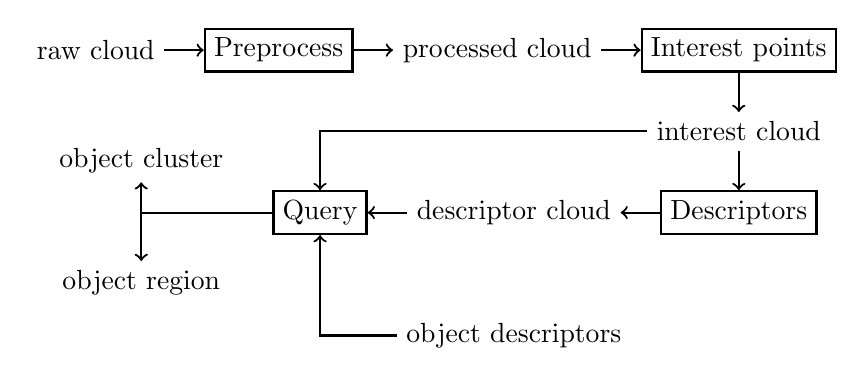
\begin{tikzpicture}
    \node[] (raw) {raw cloud};

    \node[draw,rectangle,thick,right=0.5cm of raw] (pre) {Preprocess};
    \node[right=0.5cm of pre] (proc) {processed cloud};
    \node[draw,rectangle,thick,right=0.5cm of proc] (interest) {Interest points};
    \node[below=0.5cm of interest] (intc) {interest cloud};
    \node[draw,rectangle,thick,below=0.5cm of intc] (desc) {Descriptors};
    \node[left=0.5cm of desc] (desccl) {descriptor cloud};
    \node[draw,rectangle,thick,left=0.5cm of desccl] (query) {Query};
    \node[above left=0.1cm and 0.5cm of query] (cluster) {object cluster};
    \node[below=1cm of cluster] (region) {object region};

    \node[below=1cm of desccl] (objdesc) {object descriptors};
  
    % arrows
    \draw[->,thick] (raw) -- (pre);
    \draw[->,thick] (pre) -- (proc);
    \draw[->,thick] (proc) -- (interest);
    \draw[->,thick] (interest) -- (intc);
    \draw[->,thick] (intc) -- (desc);
    \draw[->,thick] (desc) -- (desccl);
    \draw[->,thick] (desccl) -- (query);
    \draw[->,thick] (query) -| (cluster);
    \draw[->,thick] (query) -| (region);
    \draw[->,thick] (objdesc) -| (query);
    \draw[->,thick] (intc) -| (query);

  \end{tikzpicture}
  \caption{Basic diagram of the system process. The object descriptors are
    extracted using the same three initial steps of preprocessing, interest
    point extraction and descriptor computation.}
  \label{fig:sysflow}
\end{figure}

In chapter~\ref{chap:bg}, we explain some concepts that are important to
understand the work, provide background information on relevant parts of the
image processing literature, and attempt to introduce the reader to previous
work in similar areas. The preprocessing steps that we apply to clouds are
described in chapter~\ref{chap:preprocess}. Brief descriptions of the interest
points and descriptors that we use are given in chapters~\ref{chap:interest} and
\ref{chap:descriptors} along with some explanation as to why we wish to use
these methods. Chapter~\ref{chap:query} is the final chapter describing our
system, wherein we discuss our approach to using descriptors to retrieve
objects. Finally, we summarise the system and our results in
chapter~\ref{chap:conc}, and suggest some potential improvements and extensions.
Our experimental setup and the results of the experiments are described in
appendix~\ref{chap:exp}. We compare the quality of retrieval when different
methods are used, and also investigate the time taken by the system under
varying parameter settings.
\chapter{Background}
\label{chap:bg}
In this chapter we will introduce some key ideas relating to the project, and
papers which are related to what we are interested in doing. While some of the
techniques mentioned here are not directly used in the implementation of our
system, they can be useful for context, or to give examples of different ways of
approaching problems in this area. We discuss methods of finding interesting
regions in image and point cloud data, and how these regions can be represented
using descriptors, along with some methods for storing descriptors in ways that
make it easy and efficient to find similarities.

\section{Point Clouds}
The most important data structure in this project is the point cloud. A point
cloud consists of points in 3D space, with $x$, $y$ and $z$ coordinates.
Depending on the way the data was gathered, there may be additional information
such as RGB data for the colour at that specific point, or intensity information
in the case of greyscale data. Point clouds can be gathered in several ways, but
recently the most common approach is to use an RGB-D camera such as the
Microsoft Kinect. To gather 3D data from a scene, an infrared grid is projected
by the camera onto the scene. Using variations in the size and distribution of
points on the grid, the depth at each point is computed in hardware. This data
is then combined with RGB information from another camera to create the point
cloud. The resulting point cloud is called a \emph{frame}. The camera is able to
create around 10 frames per second, depending on the resolution.

\section{Segmentation}
Segmentation encompasses techniques for splitting an image or a point cloud into
different parts, or grouping similar parts --- this is essentially two sides of
the same coin. In terms of images, segmentation might be used to try to find
background and foreground pixels, or for point clouds, to separate objects from
the surfaces on which they are resting. There are many different types of
methods in the area, which approach the problem from different starting points.

\begin{figure}
  \centerline{
    \subfloat[Superpixels size 64, 256 and 1024 computed using SLIC \cite{achanta2012slic}]{
      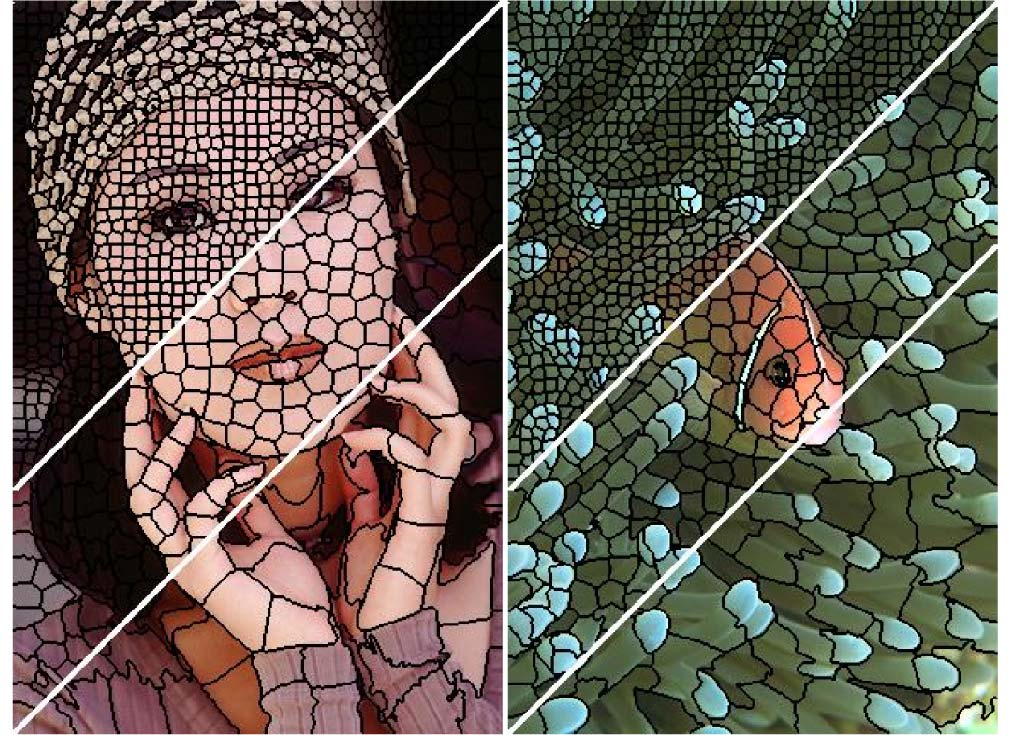
\includegraphics[height=0.3\textheight]{images/slic}
    }
    \subfloat[Supervoxel oversegmentation \cite{papon2013voxel}]{
      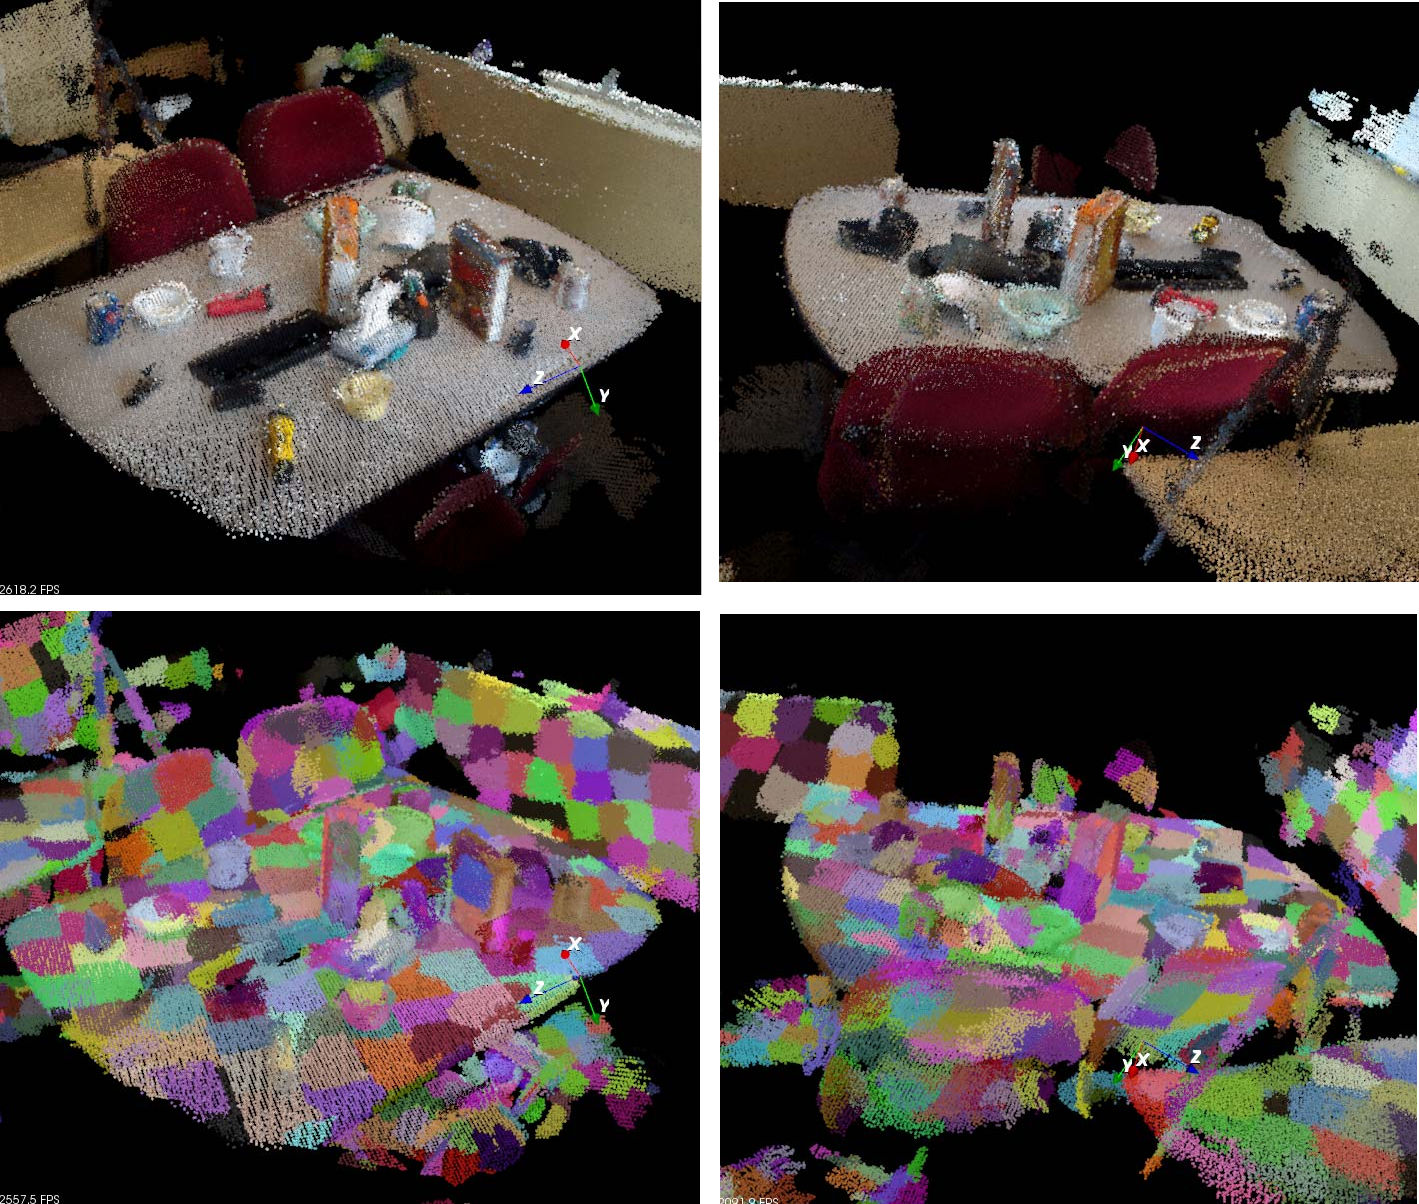
\includegraphics[height=0.3\textheight]{images/supervoxel_comb}
    }
  }
  \caption{Examples of 2D and 3D superpixel segmentations}
  \label{fig:supervoxel}
\end{figure}

Superpixel clustering is the most common technique used for segmenting images.
The intent is to create regions in which all pixels have some sort of meaningful
relationship. Graph based algorithms treat pixels as nodes in a graph, where the
weights on edges between nodes are related to the similarity between the
connected pixels --- intensity, proximity and so on \cite{achanta2012slic}. The
most simple method is to use a threshold on the edge weights to create
superpixels. Fulkerson et al. use superpixel methods to identify object classes
in images \cite{fulkerson2009class}. An algorithm which applies the idea of
superpixels to point clouds to create supervoxels (3D pixels) has also been
developed \cite{papon2013voxel}. An example of supervoxels is shown in
Figure~\ref{fig:supervoxel}.

Gradient ascent based algorithms iteratively improve clusters until some
criterion for convergence is reached \cite{achanta2012slic}. Popularised by
Comaniciu~\cite{comaniciu2002mean}, mean shift was first introduced by
Fukunaga~\cite{fukunaga1975estimation} in 1975, and rediscovered by
Cheng~\cite{cheng1995mean} in 1995. The technique finds stationary points in a
density estimate of the feature space, for example pixel RGB values, and uses
those points to define regions in the space by allocating pixels to them. One
common way of computing a density estimate is to place Gaussians at the location
of each pixel, and then to sum the values of all the Gaussians over the entire
space. Pixels which follow the gradient of the density to the same stationary
point are part of the same segment. An example can be seen in
Figure~\ref{fig:meanshift}.
\begin{figure}[t]
  \centering
  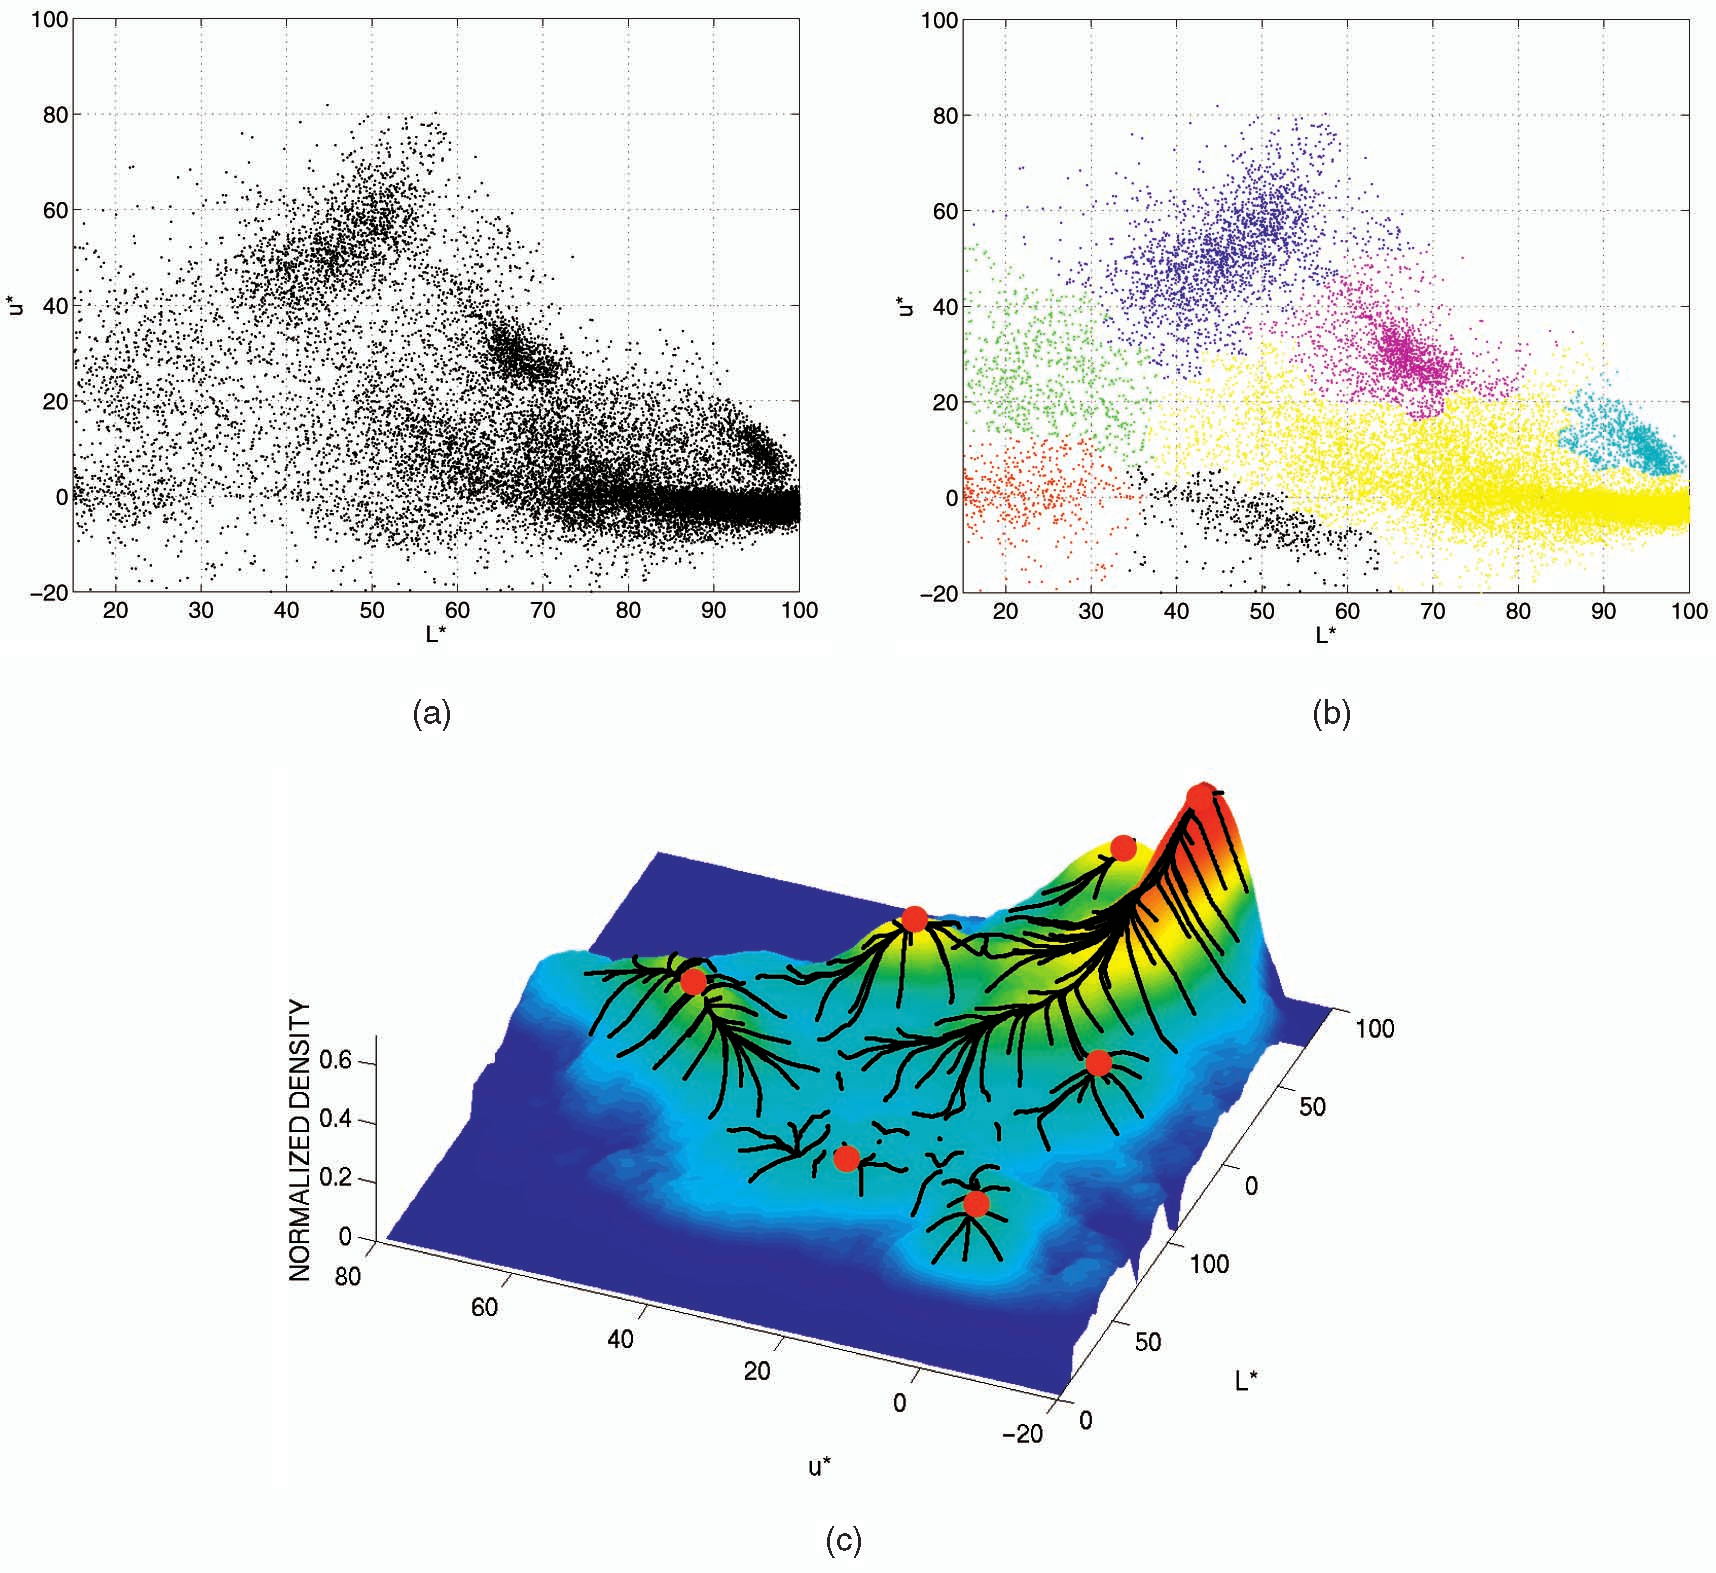
\includegraphics[width=\textwidth]{images/meanshift}
  \caption{Visualisation of mean shift \cite{comaniciu2002mean}. a) First two
    components of image pixels in LUV space. b) Decomposition found by running
    mean shift. c) Trajectories of mean shift over the density estimate.}
  \label{fig:meanshift}
\end{figure}


Random Sample Consensus (RANSAC) is a technique which uses shape models to find
ideal models in noisy data. Points in the data set are randomly sampled, and
used to construct a shape. For example, in the case of a line, two points are
sampled, and define the line. Distances from points in the data set to the model
defined by the randomly sampled points are then computed to find points which
are inliers to the model. This number is stored, and the process repeated a
number of times. At the end of the process, the model with the largest number of
inliers is returned \cite{fischler1981random}. RANSAC can be applied to
segmentation tasks by using it to find planes, cylinders, spheres and so on in
point clouds. In the case of planes this is particularly useful, as they are
usually not part of objects of interest, mostly making up walls, floors or
surfaces on which interesting objects rest. By removing the points corresponding
to these uninteresting surfaces, it should be possible to work only with parts
of clouds that contain objects of interest.

Several extensions to RANSAC have been proposed. Maximum Likelihood Estimation
Sample Consensus (MLESAC) chooses a solution that maximises the likelihood of
the model instead of just the number of inliers \cite{torr2000mlesac}.
M-estimator Sample Consensus (MSAC) uses a different cost function to the
original implementation, additionally scoring the inliers depending on how well
they fit the data \cite{torr2000mlesac}. The Progressive Sample Consensus
(PROSAC) uses prior information about the likelihood of input data being an
inlier or an outlier to limit the sampling pool and greatly reduce computation
cost \cite{chum2005matching}.


\section{Interest Points and Saliency}
Interest points are an important concept in many image processing applications,
and often form part of two stage process for extracting descriptor information
from images or scenes. As the name suggests, techniques which use this approach
try to find points in the image which are interesting, by some measure. This can
be any of a number of things, depending on the types of images or objects that
are being described. The general idea is that regions which have extreme values
for some measure like intensity or curvature are more likely to be picked up
later when the same object is observed in another image. This is very important,
as when computing descriptors one would like to extract them at the same points
on the same objects every time in order to ensure that two instances of the
object can be matched.

Sipiran and Bustos extend the popular Harris detector \cite{harris1988combined}
to 3D \cite{sipiran2011harris}. The original detector for 2D finds edges and
corners in images by computing a matrix of the sum of squared distances between
points in one patch of an image, and points in a shifted copy of this patch.
Interest points are then selected using the eigenvalues of these matrices. The
extended 3D version uses normals to do the computation.

The SUSAN detector \cite{smith1997susan} uses sub-regions of circular masks
placed on an image to define a value for the intensity variation in a region.
This method is extended to 3D by combining normal direction variation with
intensity variation and using a spherical mask.

A multi-scale signature defined by the heat diffusion properties of objects 
called the Heat Kernel Signature (HKS) \cite{sun2009concise} is used in
\cite{ovsjanikov2009shape} to retrieve shapes. The method is applied to meshes
and is robust to deformations of the shape, which is particularly important for
model matching.

Shilane and Funkhouser introduce a distinctiveness measure over classes of
meshed objects which uses a database of existing objects to compute the
distinctiveness of descriptors computed all over the object, based on how
similar descriptors are to those inside the class compared to those from other
classes. This distinctiveness measure is then used to discriminate between
different classes of objects \cite{shilane2007distinctive}.

Zhong introduces an interest point selection method specifically for 3D, which
uses the covariance matrix to define the region around a point, and extracts
information about the region using the eigenvalues \cite{zhong2009intrinsic}.

\section{Descriptors}
The problem of describing regions of an image in a compact and useful manner has
been studied for a long time in the computer vision community. For any given
point in an image, we would like to create a description which can be used to
represent the region around the point in some way. This descriptor, or feature,
can then be compared to other descriptors to see if there is some similarity. If
the similarity is within a given threshold, then we can assume that the points
represented by the two descriptors come from the same object, or represent the
same thing in both images. Thus, it is important to create features which are
distinct for different regions. In addition, since objects move around and can
be seen from different sides, or in different lights, an attractive property of
descriptors is to give similar results for the same region which has been
transformed in some way. In practice, this is quite difficult to achieve.
\subsection{2D}
While 2D descriptors are not directly usable on point clouds, the ideas that
they use to give effective results can be transferred over to use for 3D
description.

The Laplacian of Gaussians was introduced by Lindeberg, and uses derivatives
combined with some other techniques to select interest points \cite{lindeberg1998feature}. This paper also introduces the concept of automatic
scale selection for feature detection, which has played an important part in the
field since then. The scale of features can be investigated by blurring an image
using a Gaussian kernel --- higher standard deviation blurs the image more,
resulting in the removal of small scale features.

Even today the Scale Invariant Feature Transform (SIFT) is among the most
popular descriptors for 2D images. It is invariant to scale and rotation, and is
robust to some variation in affine distortion, viewpoint and illumination, and
is distinctive, allowing for correct matching of single features in large
databases. There are several stages of computation. Extrema are found in
different scales to find points invariant to scale and orientation. Keypoints
are selected at the extrema based on their stability. Image gradients at the
keypoint are used to define its orientation for future computations. The image
gradients are then transformed into a local descriptor vector with length 128
\cite{lowe2004distinctive}.

Mikolajczyk and Schmid~\cite{mikolajczyk2004scale} introduce the Harris-Laplace
detector which is an improvement on SIFT \cite{lowe2004distinctive} and the
Laplacian of Gaussians \cite{lindeberg1998feature} in the sense that it is able
to deal with affine transformations. They do not, however, introduce a new type
of descriptor to go with the point selection. 

Speeded-Up Robust Features (SURF) is a more recent descriptor which can be
computed and compared much faster than most other descriptors. It makes use of
integral images, which replace pixels in an image or image patch with a
cumulative sum of the pixel intensities over the rows and columns. This allows
for fast computation of pixel intensities in an area of the image. SURF takes
some ideas from SIFT, using the spatial distribution of gradients as a
descriptor, but integrates over the gradients instead of using individual
values, which makes it more robust to noise. The resulting descriptor is a 64
element vector, which means that it is also faster to compare than SIFT
\cite{bay2008speeded}.



\subsection{3D}
\begin{figure}
  \centering
  \subfloat{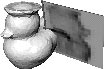
\includegraphics[width=0.11\textwidth]{images/spin1}}
  \subfloat{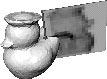
\includegraphics[width=0.11\textwidth]{images/spin2}}
  \subfloat{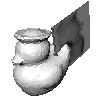
\includegraphics[width=0.11\textwidth]{images/spin3}}
  \subfloat{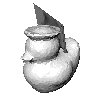
\includegraphics[width=0.11\textwidth]{images/spin4}}
  \subfloat{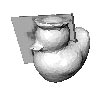
\includegraphics[width=0.11\textwidth]{images/spin5}}
  \subfloat{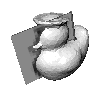
\includegraphics[width=0.11\textwidth]{images/spin6}}
  \subfloat{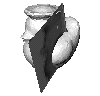
\includegraphics[width=0.11\textwidth]{images/spin7}}
  \subfloat{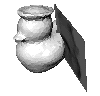
\includegraphics[width=0.11\textwidth]{images/spin8}}
  \caption{Frames from construction of a spin image \cite{johnson1997spin}. The
    image plane spins around the oriented point normal and accumulates points.}
  \label{fig:spinimg}
\end{figure}

One early descriptor which remains popular is the spin image. The descriptor is
generated from a mesh model at oriented points with a surface normal. A plane
intersecting the normal with a certain width and height is rotated around the
normal, forming a cylinder. The plane is separated into bins. The bins
accumulate the number of points which pass through a certain bin during the
rotation. The resulting 2D image is the descriptor. By varying the width of the
plane the region which defines the descriptor can be modified. A small width
will give a local descriptor, while a large width will give a descriptor for the
whole image \cite{johnson1997spin,johnson1999using}. Figure~\ref{fig:spinimg}
shows a visualisation of how the image is generated.

The Ensemble of Shape Functions (ESF) descriptor introduced in
\cite{wohlkinger2011ensemble} by Wohlkinger and Vincze combines the Shape
Distribution approach introduced by \cite{osada2002shape} along with some
extensions proposed in \cite{ip2002using}. It also makes use of their
voxel-based distance measure from \cite{wohlkinger2011shapedist}. Pairs or
triples of points are sampled from segmented partial clouds of objects, and
histograms are created by extracting information such as distance, angle,
ratios, and whether points are inside or outside (or a mix) of the model, as
shown in Figure~\ref{fig:wohlESF}.

\begin{figure}
  \centering
  \subfloat[]{
    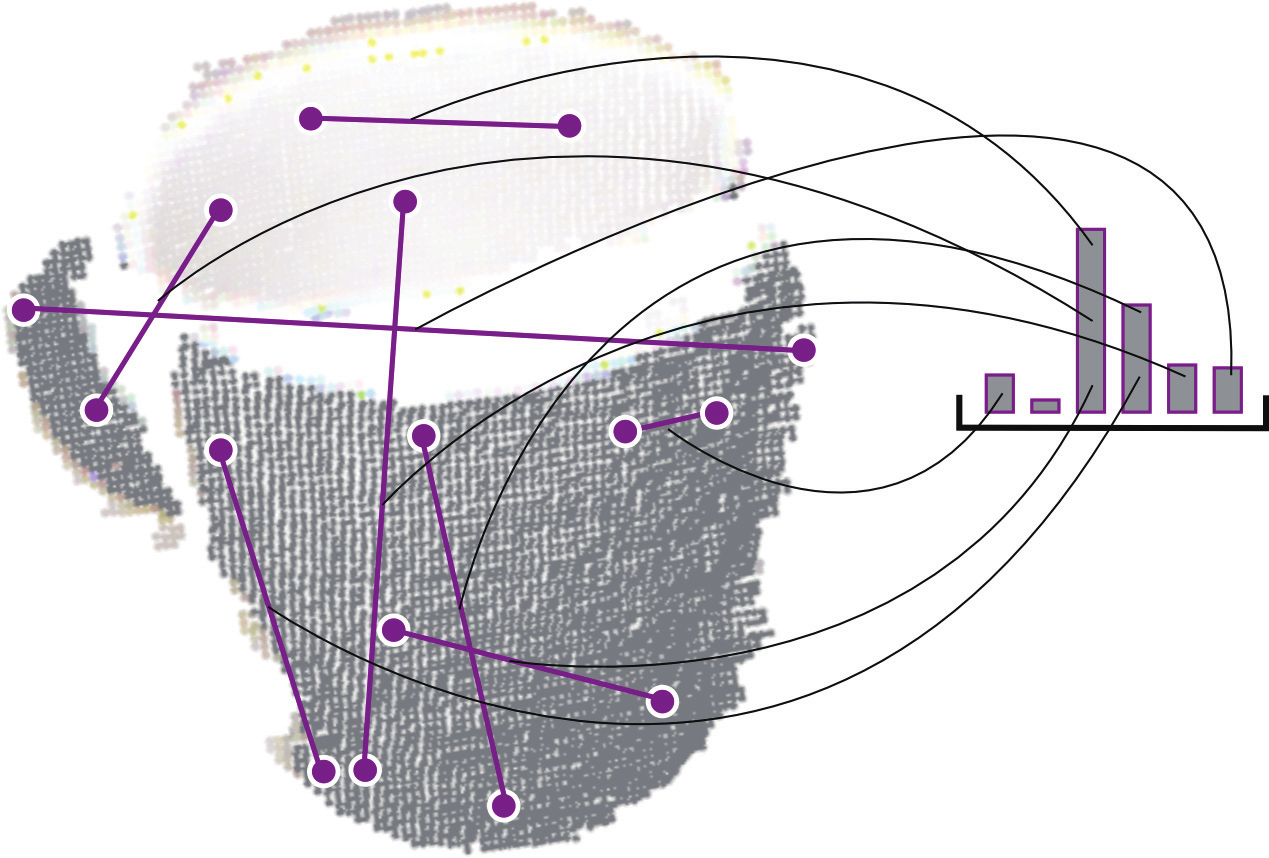
\includegraphics[width=0.23\textwidth]{images/wohl_d2}
  }
  \subfloat[]{
    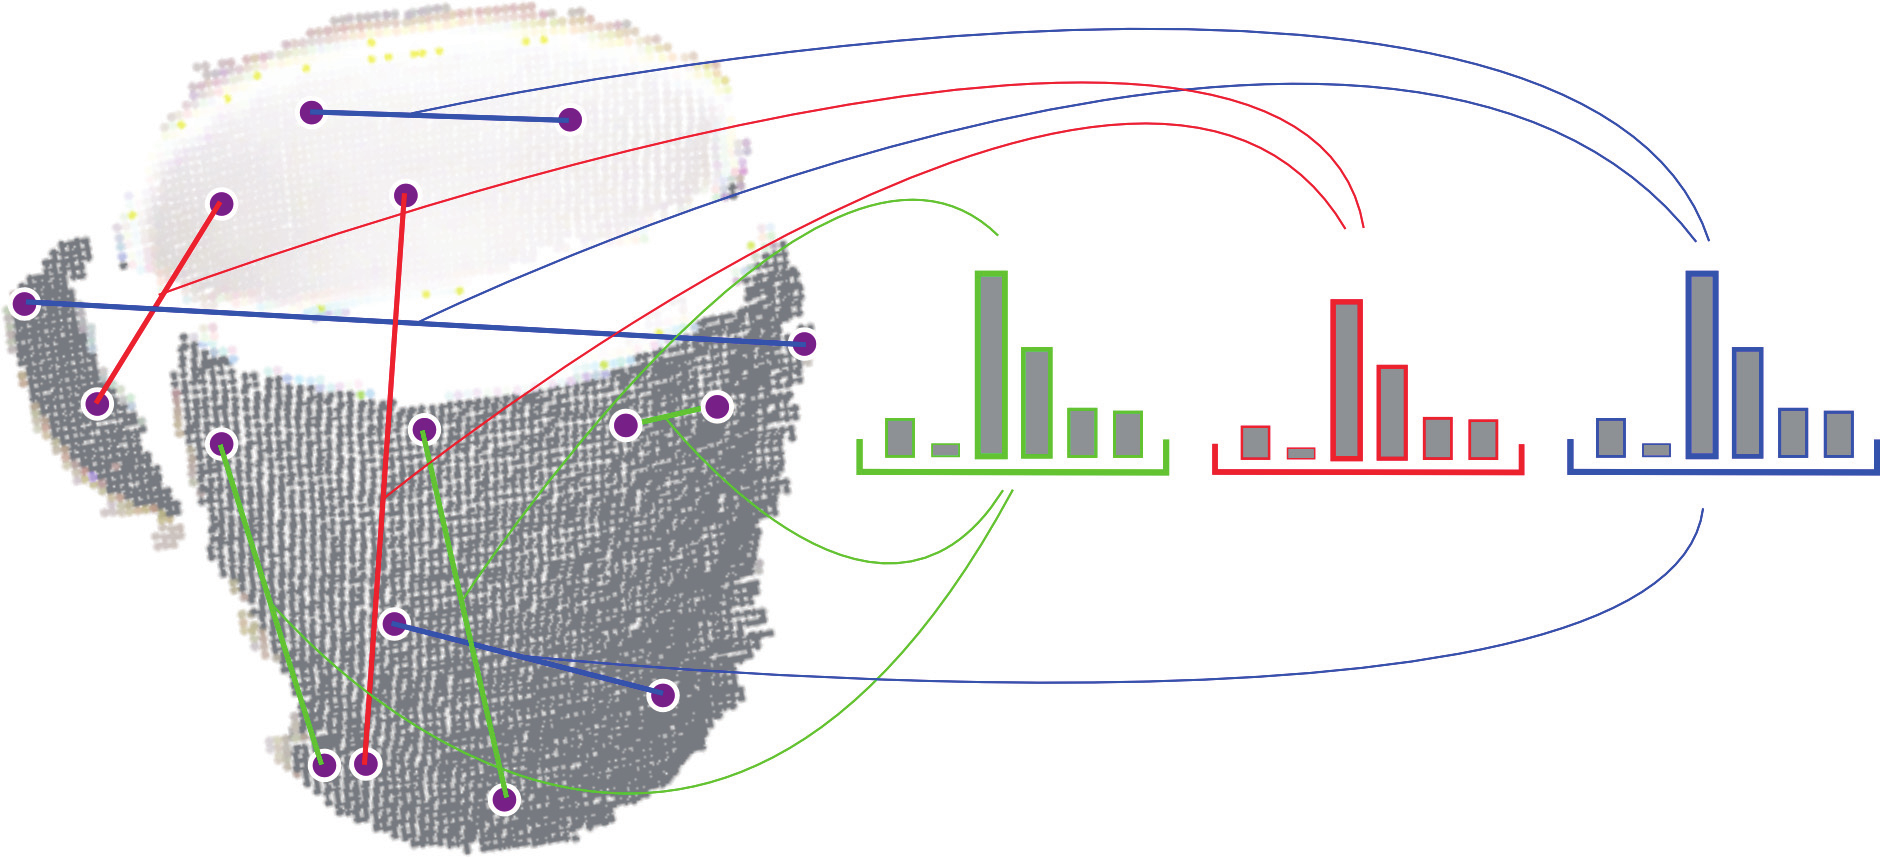
\includegraphics[width=0.23\textwidth]{images/wohl_onoff}
  }
  \subfloat[]{
    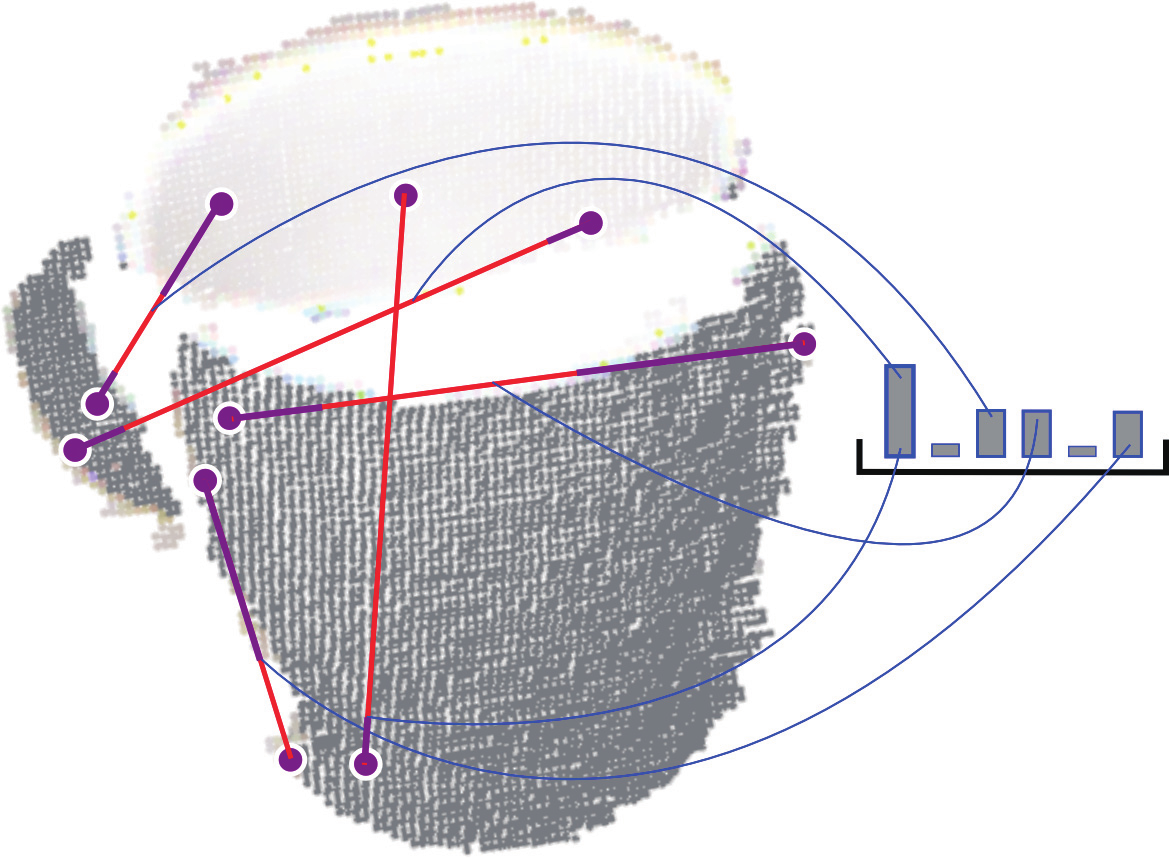
\includegraphics[width=0.23\textwidth]{images/wohl_ratio}
  }
  \subfloat[]{
    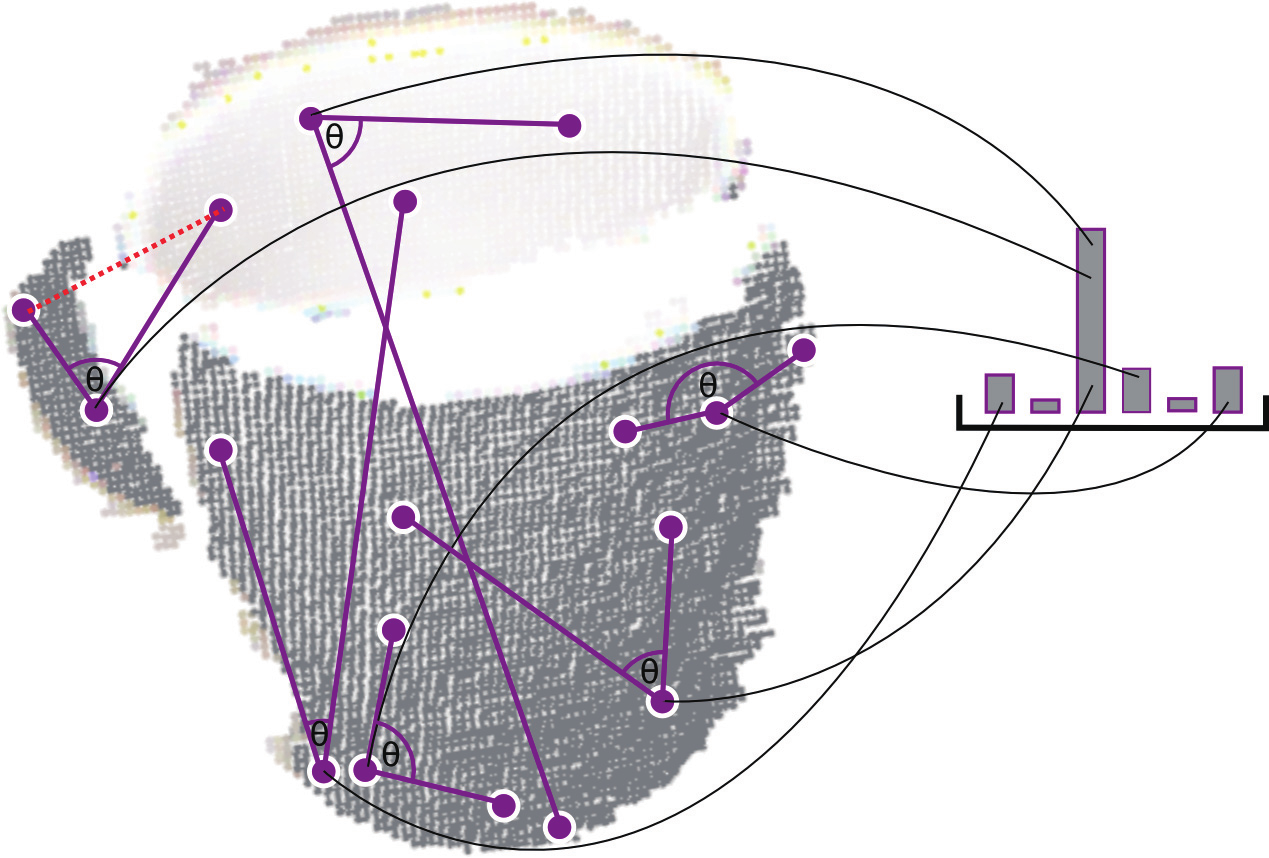
\includegraphics[width=0.23\textwidth]{images/wohl_a3}
  }
  \caption{Examples of the measures used to construct the Ensemble of Shape
    Functions histograms of \cite{wohlkinger2011ensemble}. a) Distance between
    points. b) Whether the points are on or off the model, or mixed. c) Ratio of
    line segments on and off the surface of the model. d) Angle between pairs of lines.}
  \label{fig:wohlESF}
\end{figure}

The Point Feature Histogram (PFH) was introduced by Rusu et al. in
\cite{rusu2008persistent}. It creates descriptors based on the angles between a
point on a surface and $k$ points close to it. The Fast Point Feature Histogram
(FPFH) improved the speed of computation, and allowed the use of the descriptor
in real time \cite{rusu2009fast}. The Viewpoint Feature Histogram (VFH) extended
the FPFH by adding viewpoint information to the histogram by computing
statistics of surface normals relative to the viewpoint \cite{rusu2010fast}. It
also improved the speed of the FPFH. The clustered version (CVFH) further
improved the viewpoint technique by mitigating the effect of missing parts and
extending it to facilitate estimation of the rotation of objects \cite{aldoma2011cad}.

Bo et al. develop the kernel descriptor initially created for RGB images for use
on depth images and point clouds. The kernels are used to describe size, shape
and edge features. Local features are combined to object-level features. Kernel
descriptors avoid the need to quantise attributes. Similarity is instead defined
by a match kernel \cite{bo2010kernel}, which improves recognition accuracy
\cite{bo2011depth}.

The point pair feature describes the relation between two oriented points on a
model. This means that it does not depend so much on the quality and resolution
of the model data. The model is described by grouping the point pair features of
the model, providing a global distribution of all the features on the model
surface \cite{drost2010model}.

\begin{figure}
  \centering
  \subfloat[3DSC \cite{frome2004recognizing}]{
    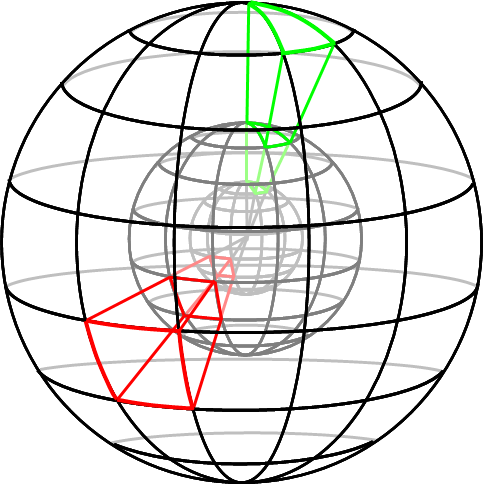
\includegraphics[width=0.24\textwidth]{images/3dsc}
    \label{fig:3dsc}
  }
  \subfloat[SHOT \cite{tombari2010unique}]{
    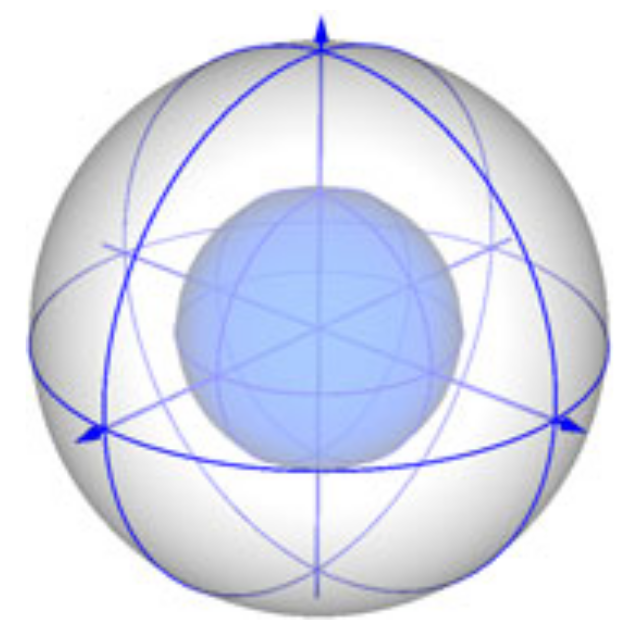
\includegraphics[width=0.24\textwidth]{images/shot}
    \label{fig:shot}
  }
  \subfloat[Context Shape \cite{shentu2008context}]{
    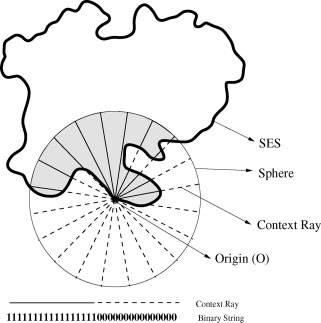
\includegraphics[width=0.24\textwidth]{images/contextshape}
    \label{fig:contextshape}
  }
  \subfloat[Integral Volume \cite{gelfand2005robust}]{
    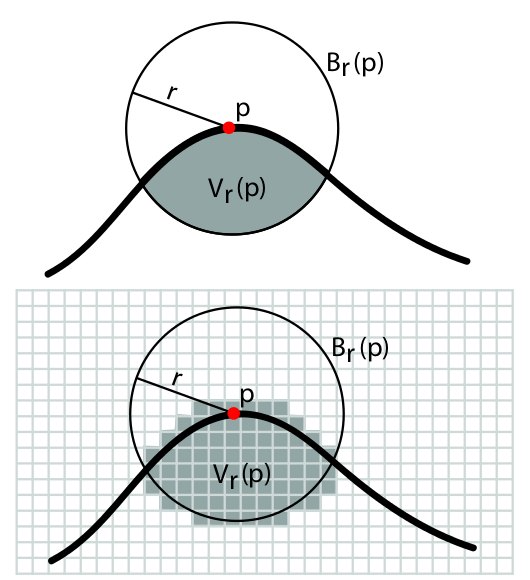
\includegraphics[width=0.24\textwidth]{images/volint}
    \label{fig:volint}
  }
  \caption{Visualisation of spherical descriptors.}
  \label{fig:descexample}
\end{figure}

3D Shape Context (3DSC) is an extension of the original Shape Context descriptor
for 2D images \cite{belongie2002shape}. A sphere is placed at a point, and its
``top'' is oriented to match the direction of the normal at the point. Bins are
created within the sphere by equally spaced boundaries in the azimuth and
elevation, and logarithmically spaced boundaries in the radial dimension (Figure~\ref{fig:3dsc}). The
logarithmic spacing means that shape distortions far from the basis point have
less effect on the descriptor. Each bin accumulates a weighted count based on
the volume of the bin and local point density \cite{frome2004recognizing}. 3DSC
does not compute a local reference frame --- the vector of the azimuth is chosen
randomly, and subdivisions computed from that. This means that a number of
descriptors equal to the number of azimuth divisions need to be computed and
stored in order to compensate, and the matching process is complicated as a
result. The Unique Shape Context (USC) solves this problem by defining a local
reference frame and using the directions of that reference frame to subdivide
the sphere \cite{tombari2010uniquesc}.

The Signature of Histograms of Orientations (SHOT) descriptor improves on 3DSC
by taking inspiration from SIFT and making extensive use of histograms. The
sphere is split into 32 volumes: 8 azimuth regions, 2 elevation and 2 radial
(Figure~\ref{fig:shot}). A local histogram is computed in each of the regions,
using the angle between the normal of points and the feature point. The local
histograms are then combined to form the final descriptor
\cite{tombari2010unique}. The authors also extend the descriptor to include
colour (COLORSHOT) \cite{tombari2011combined}.

The Rotation Invariant Feature Transform (RIFT) is a generalisation of SIFT. Using
intensity values computed at each point from the RGB values, a gradient is
computed. Concentric rings are placed around the initial point, and a histogram
of the gradient orientations is created for points within each ring. The
orientation of the gradient is computed relative to the line from the central
point so that the descriptor is rotation invariant. The descriptor is 2D --- one
dimension is the distance, the other the gradient angle. The distance between
two descriptors is measured using the earth mover's distance (EMD), which is a
measure of the distance between two probability distributions
\cite{lazebnik2005sparse}.

Multi-scale descriptors are useful as they can be used to characterise regions
of varying size. Cipriano et al. introduce such a descriptor for use on meshes
\cite{cipriano2009multi}. It captures the statistics of the shape of the
neighbourhood of a vertex by fitting a quadratic surface to it. Vertices in the
region are weighted based on distance from an initial vertex, and a plane is
constructed using a weighted average of the face normals. The parameters of the
quadratic are then used to find its principle curvatures, which make up the
descriptor.

Work in protein-protein docking also uses 3D descriptors to help with
simulations of an otherwise lengthy and complex process. The Surface Histogram
is introduced by Gu et al. \cite{gu2012surface}, and uses the local geometry
around two points with specific normals on the surface of a protein. A
coordinate system is defined by the two points and the line between them, and a
rectangular voxel grid is defined around the points. The grid is then marked in
locations where the surface crosses the grid, and a 2D image is constructed by
squashing the data onto one of the axes. The descriptor is designed to
immediately give a potential pose for the docking.

Another example of a shape descriptor from biology is the Context Shape
\cite{shentu2008context}. A sphere is centred on a point, and rays are projected
from this point to points evenly distributed on the surface of the sphere (Figure~\ref{fig:contextshape}). Each
of the rays is divided into segments, with a binary value associated with each
segment depending on whether the segment is inside or outside the protein. To
compare the descriptor, a rotation is applied to match the rays, and a volume of
overlap is computed based on matching bits in the rays.

The splash descriptor was introduced by Stein et al. \cite{stein1992structural}.
A point on the surface with a given surface normal (the reference normal) is
chosen, and a slice around that with some geodesic radius (distance along the
surface) is computed. Points on the circle are selected using some angle step,
and the normal at that point is determined. A super splash is when this process
is repeated for several different radii. For each normal on the circle,
additional angles between it and a coordinate system centred on the reference
normal are computed. These angles and the angle around the circle are then
mapped into a 3D space, where polygonal approximation is made, connecting each
point with a straight line. Some additional computation is done to allow the
encoded polygons to act as a hash. Figure~\ref{fig:splash} shows part of the
formulation.

\begin{figure}
  \centering
  \subfloat[]{
    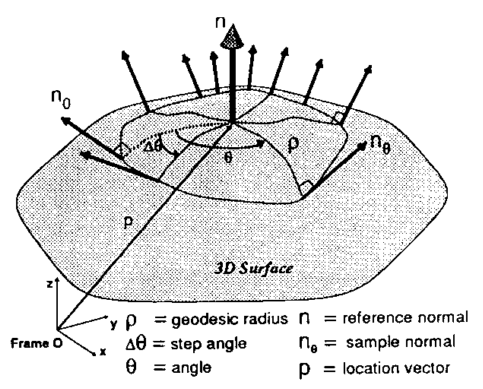
\includegraphics[width=0.32\textwidth]{images/splash}
  }
  \subfloat[]{
    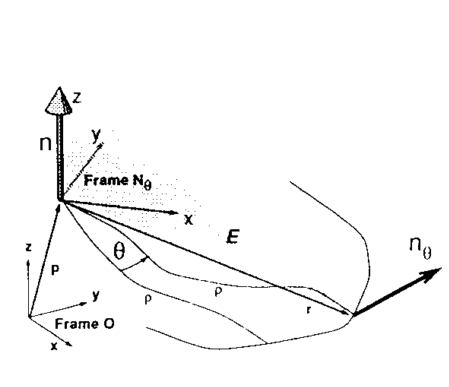
\includegraphics[width=0.32\textwidth]{images/splash_normals}
  }
  \subfloat[]{
    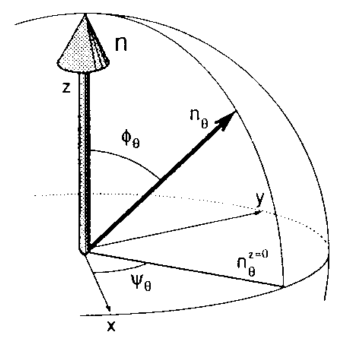
\includegraphics[width=0.32\textwidth]{images/splash_angles}
  }
  \caption{Splash descriptor \cite{stein1992structural}. a) shows the splash and
    normals around it. b) and c) show how the additional angles are defined.
  }
  \label{fig:splash}
\end{figure}

Point Signatures are similar to the splash descriptor in the sense that they
both sample points on a circle \cite{chua1997point}. This descriptor again
selects a reference normal, and has a specific radius. This time, the radius
defines a sphere around the point. The intersection of the surface with the
sphere is a 3D space curve. The orientation of the curve is defined by fitting a
plane to it. The distances between the space curve and the fitted plane at
sampled points define the signature of the reference point. These signatures can
be compared by lining them up and checking whether the query falls within the
tolerance band of previous signatures. Figure~\ref{fig:pointsig} shows
signatures from various surfaces.

\begin{figure}
  \centering
  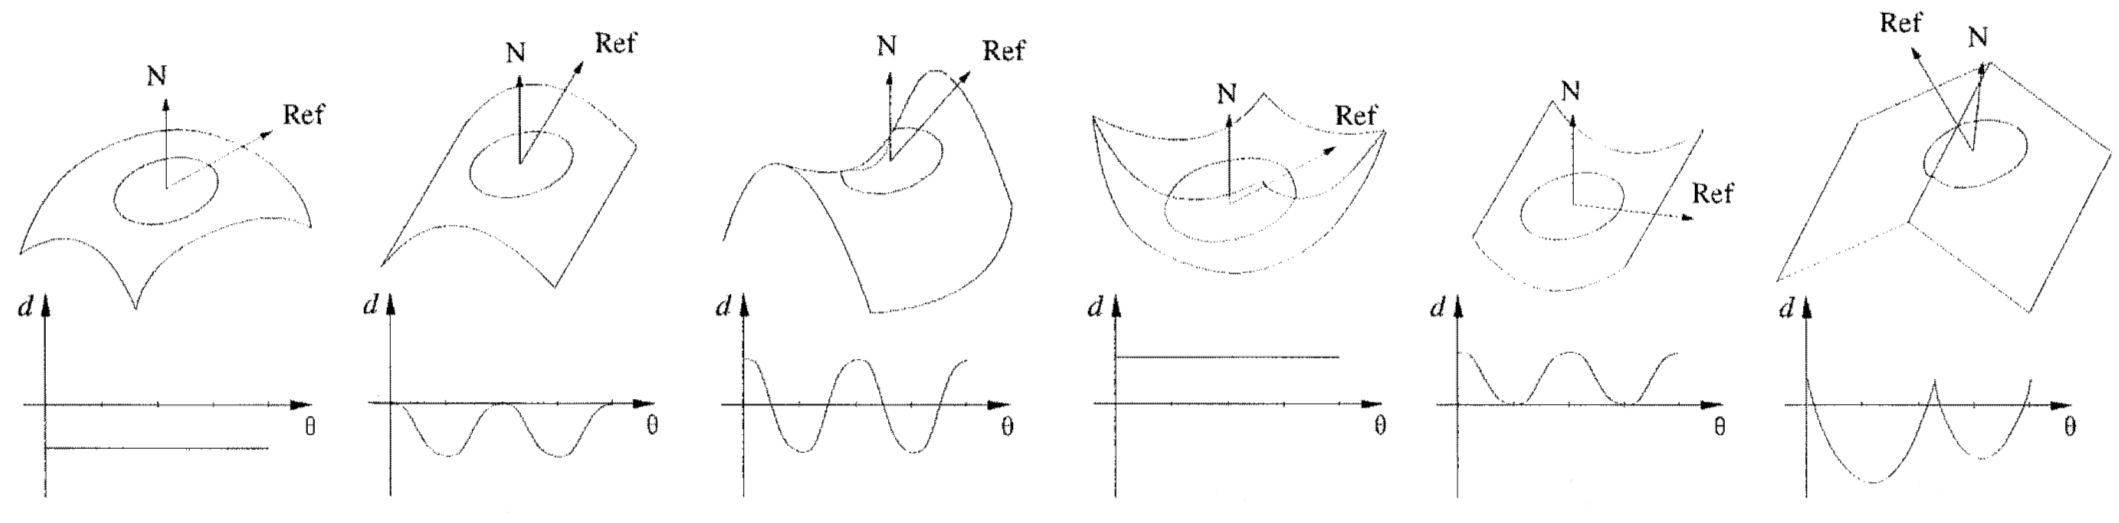
\includegraphics[width=\textwidth]{images/pointsig}
  \caption{Examples of the point signature responses to different surfaces
    \cite{chua1997point}. $d$ is the distance from the reference vector to the
    space curve defined by the intersection of the surface with a sphere centred
    at $N$. Ref rotates about $N$.}
  \label{fig:pointsig}
\end{figure}

\subsubsection{Descriptors With Interest Point Extraction}
While many descriptors designed for 2D applications also select interest points
during an initial step in the process, the 3D descriptors that we have mentioned
above do not automatically find locations in the cloud which are good points at
which to compute descriptors.

The Normal Aligned Radial Feature (NARF) is an interest point extraction method
with a feature descriptor. A score for the image points is determined based on
the surface changes at the point, and information about borders. An interest
value is computed from this based on the score of the surrounding points.
Smoothing is applied, and non-maximum suppression is applied to find the final
interest points. To compute the descriptor, rays are projected over the range
image from the centre at certain intervals. The intensities of cells lying under
the ray are weighted based on their distance from the centre, and a normalised
weighted average of the pairwise difference of cells is used to define each
element of the descriptor vector, which has a length equal to the number of rays
\cite{steder2011point}. The method is an improvement on a previous paper by the
authors \cite{steder2009robust}. A problem with this method is that it uses
range images directly. Point clouds can be used to generate range images by
looking at them from different viewpoints, but this adds complexity to the
method.

The integral volume descriptor is interesting as it combines interest point
selection and description into one. The descriptor is defined as the volume of
the intersection of a sphere centred at a point on the surface of an object with
the inside of the object (Figure~\ref{fig:volint}). Interest points are selected
by histogramming the descriptor values, identifying bins with a number of points
less than a specified values, and selecting points from these bins. To ensure
features are properly spaced, points in a certain radius of already selected
points cannot be used. By modifying the radius of the sphere used to generate
the descriptor, interest points at different scales can be selected
\cite{gelfand2005robust}.

% \section{Matching Objects}
% \subsection{Point Matching}
% In \cite{chui2003new}, Chui and Rangarajan introduce an extension to the
% iterative closest point (ICP) method, which allows for non-rigid registration and
% improved robustness to outliers. In contrast to ICP, their approach does not use
% the nearest-neighbour approach to define correspondence. Instead, they use an
% alternating algorithm similar to expectation maximisation. Annealing is used to
% prevent binary correspondences when the algorithm is not yet close to the
% solution --- at the beginning there is a large search range for correspondences,
% which gradually shrinks as the temperature decreases.

% \subsection{Model Matching}
% \begin{figure}
%   \centering
%   \subfloat[Conformal factors. High value indicates high required deformation to
%   sphere \cite{ben2008characterizing}.]{
%   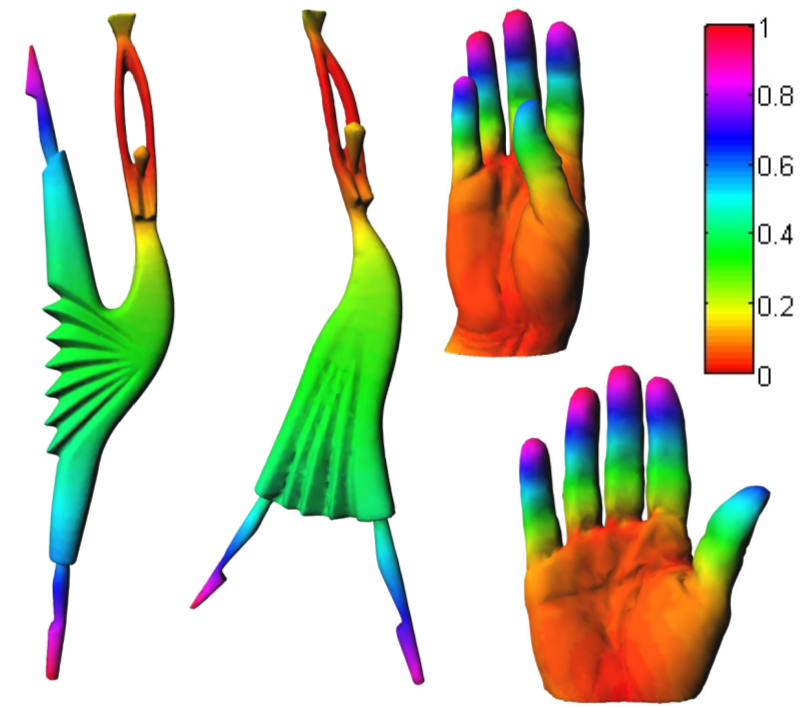
\includegraphics[width=0.48\textwidth]{images/conformal.png}
%   \label{fig:conform}
% }
%   \caption{Model matching approaches}
%   \label{fig:modelmatch}
% \end{figure}
% In \cite{ben2008characterizing}, Chen et al. describe another approach to model
% matching using conformal factors. This technique uses ideas from conformal
% geometry, transforming the mesh of an object such that it has a uniform Gaussian
% curvature. Information is stored about how much deformation is needed locally to
% globally transform the object into a sphere --- this is the conformal factor.
% The factor is based on a global computation on the whole mesh, as opposed to
% per-vertex computations of the Gaussian curvature, which makes it much smoother
% and appropriate for use in histograms. The histogram of a sample of the factors
% is used as a descriptor, and is pose invariant, as seen in
% Figure~\ref{fig:conform}. The authors say that it should be possible to use the
% approach in partial model matching.

\section{Storing and Querying Descriptors}
There are several techniques for storing and querying descriptors, mostly based
on some form of tree. Recently, the k-d tree\cite{bentley1975multidimensional,
  friedman1977algorithm} has been used for efficient approximate matching with
either an error bound \cite{arya1998optimal}, where there is a bound placed on
the error between the true nearest neighbour and the one found, or a time bound
\cite{beis1997shape}, where the search is stopped after examining a certain
number of leaf nodes. Further improvements on the k-d tree are introduced in
\cite{silpa2008optimised}, where multiple randomised trees are used to optimise
the search. A priority search tree algorithm is introduced in
\cite{muja2014scalable}, which appears to be very effective. This may be the
same one as in \cite{muja2009fast}.

A different approach to nearest neighbour search is the balltree, which uses
hyperspheres in a hierarchy to enclose points in the space
\cite{omohundro1989five}. Unlike the k-d tree, regions on the same level of the
tree are allowed to intersect, and do not need to partition the whole space,
which gives the balltree its representative power.

The vocabulary tree \cite{nister2006scalable} makes use of techniques from
document search to index images. Using $k$-means clustering, construction stage
creates a hierarchical quantisation of the image patch descriptors. In the query
phase, descriptors are compared to the cluster centres, and go down the tree
until a leaf is reached. The path through the tree is used as a scoring measure
to present retrieval results.

Philbin et al. \cite{philbin2007object} show that flat (single-level) $k$-means
clustering can be scaled to large vocabulary sizes if approximate nearest
neighbour methods are used. Early systems for image retrieval used a flat
clustering scheme, which could not scale to large vocabularies
\cite{sivic2003video}. The paper also introduces a re-ranking method which uses
spatial correspondences, which improves the retrieval quality.

Boiman et al. \cite{boiman2008defense} introduce the Naive Bayes Nearest
Neighbour (NBNN) classifier. It uses nearest neighbour distances in the space of
descriptors instead of images, computing ``image-to-class'' distances without
quantising the descriptors. In general, quantisation allows for dimensionality
reduction, at the expense of the discriminative power of descriptors. NBNN ``can
exploit the discriminative power of both (few) high and (many) low informative
descriptors''. The problem here is that the classes must be known beforehand,
and in our case we do not have that information. The local NBNN
\cite{mccann2012local} does not do the search based on classes. Instead, all the
descriptors are merged into a k-d tree on which approximate $k$-NN is run to
find descriptors in the local region of a query descriptor. A distance to
classes not present in the $k$-NN region is approximated by the distance to the
$k+1$th neighbour.

Funkhouser and Shilane present a method for querying a database of 3D objects
represented by local shape features \cite{funkhouser2006partial}. Partial
matches (correspondences) are stored in a priority queue sorted by geometric
deformation and the feature similarity. This means that only objects in the
database with a high probability of being a match need to be processed.

Some work has been done on optimising the retrieval of relevant images by
learning from user input \cite{rui2000optimizing}. When retrieved images are
presented, the user ranks them in terms of relevance, and this rank is then used
to improve the relevance of future searches.

\chapter{Preprocessing}
\label{chap:preprocess}
The first step in the object query system is to perform some preprocessing on
the clouds in the data set --- while not strictly necessary, there are some
benefits to doing so, chief of which is a reduction in computation time. The
data set that we have consists of around 80 clouds of a single room, taken at
different times during different days of approximately a month of time. The
clouds are made up of a number of intermediate frames, which are registered into
a complete cloud. The robot used to collect the clouds takes several sweeps of
the room, changing the angle of the camera after each sweep. The clouds are
constructed using frames taken from a sweep where the camera is pointing
slightly below the horizontal. Examples of the raw clouds can be seen in
Figure~\ref{fig:orig}.
\begin{figure}
  \centering
  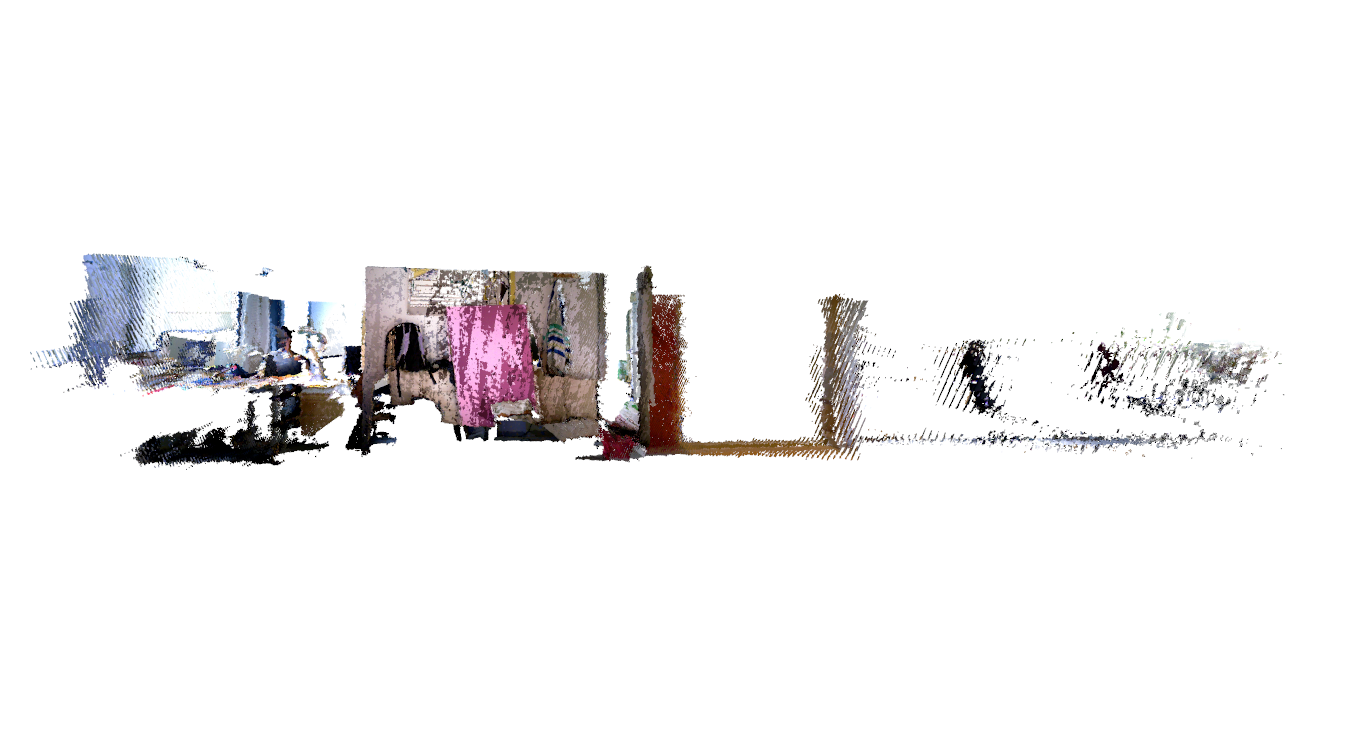
\includegraphics[width=0.9\textwidth]{images/orig_side}
  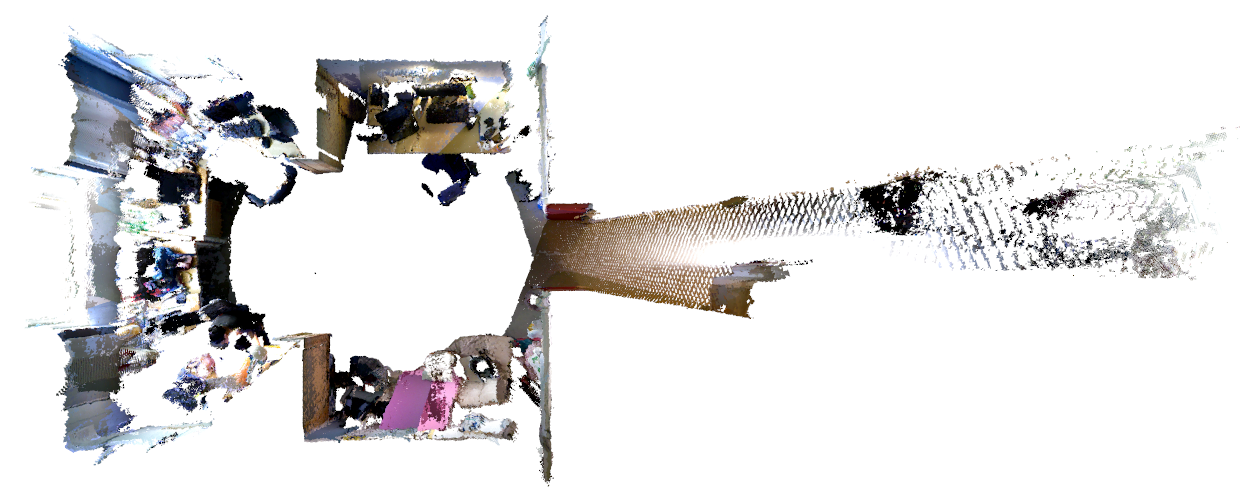
\includegraphics[width=0.9\textwidth]{images/orig_top}
  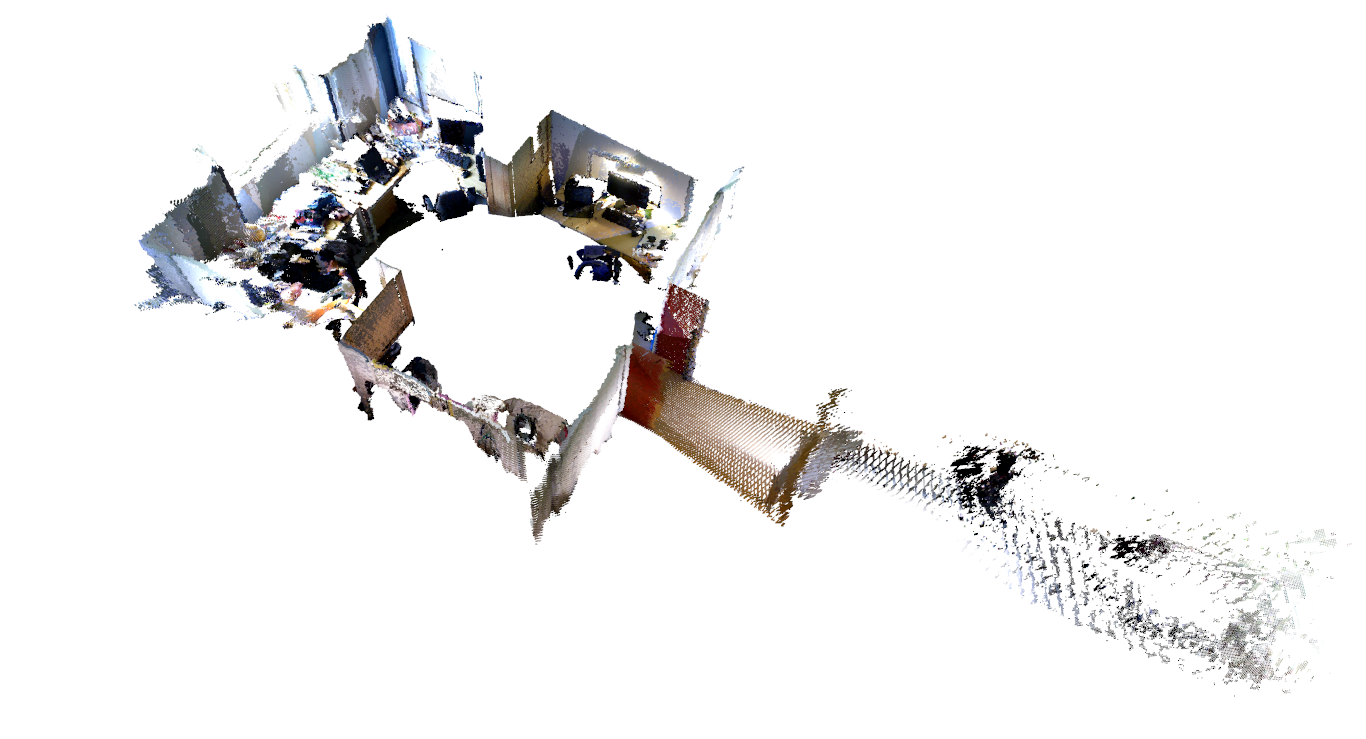
\includegraphics[width=0.9\textwidth]{images/orig_diag_left}
  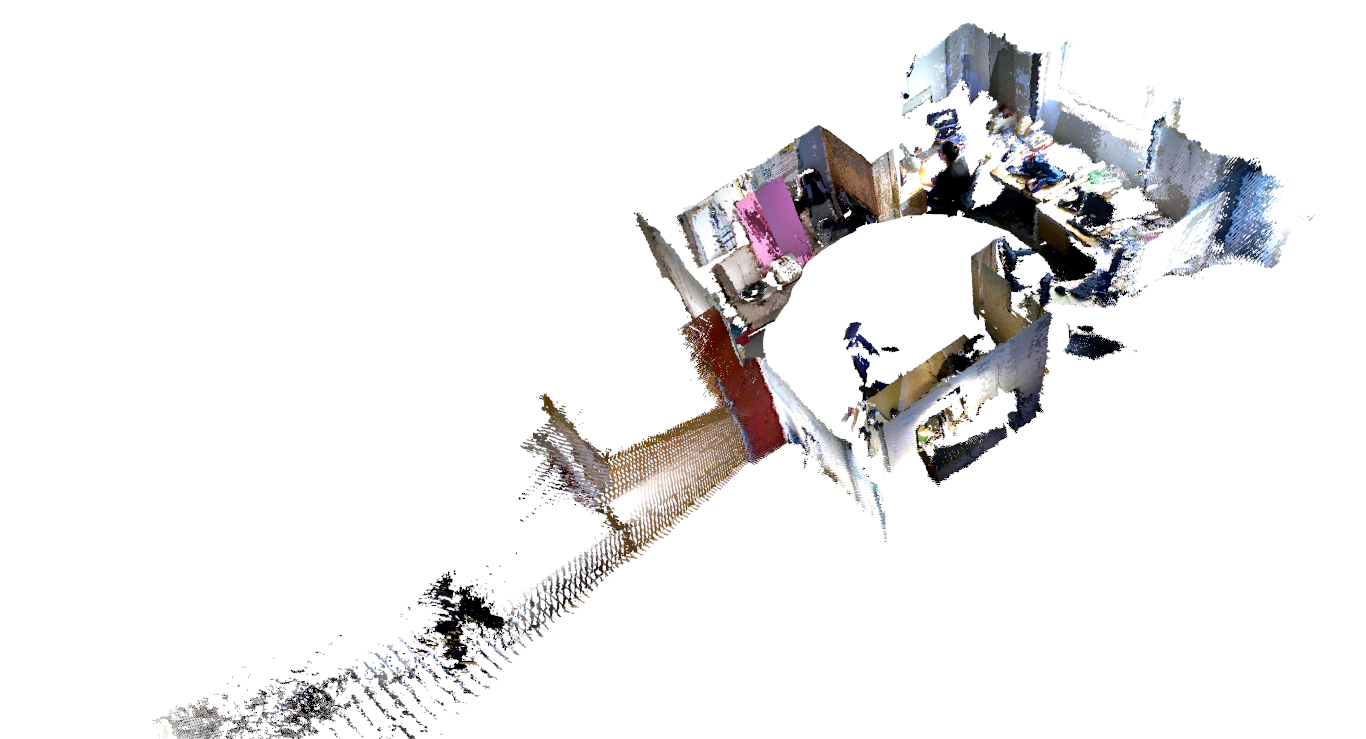
\includegraphics[width=0.9\textwidth]{images/orig_diag_right}
  \caption{Sample raw cloud from various viewpoints.}
  \label{fig:orig}
\end{figure}

% \begin{figure}
%   \centering
%   \subfloat[backpack1]{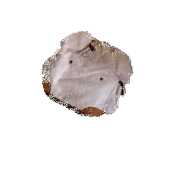
\includegraphics[width=0.30\textwidth]{images/annotations/original/backpack1_front_ut}}
%   \subfloat[backpack2]{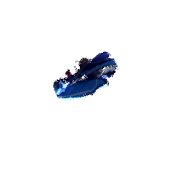
\includegraphics[width=0.30\textwidth]{images/annotations/original/backpack2_front_ut}}
%   \subfloat[helmet]{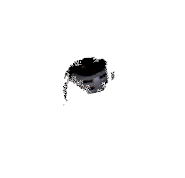
\includegraphics[width=0.30\textwidth]{images/annotations/original/helmet_front_ut}}\\
%   \subfloat[chair3]{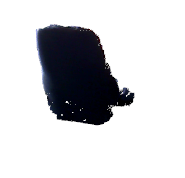
\includegraphics[width=0.30\textwidth]{images/annotations/original/chair3_front_ut}}
%   \subfloat[pillow3]{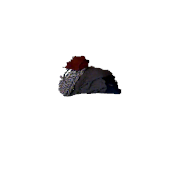
\includegraphics[width=0.30\textwidth]{images/annotations/original/pillow3_front_ut}}
%   \subfloat[laptop1]{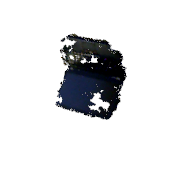
\includegraphics[width=0.30\textwidth]{images/annotations/original/laptop1_front_ut}}\\
%   \subfloat[laptop2]{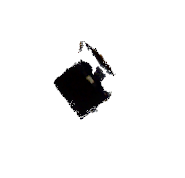
\includegraphics[width=0.30\textwidth]{images/annotations/original/laptop2_front_ut}}
%   \subfloat[hanger\_jacket]{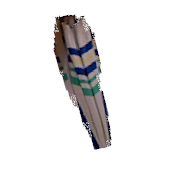
\includegraphics[width=0.30\textwidth]{images/annotations/original/hanger_jacket_front_ut}}
%   \subfloat[trash\_bin]{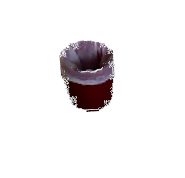
\includegraphics[width=0.30\textwidth]{images/annotations/original/trash_bin_front_ut}}\\
%   \subfloat[chair1]{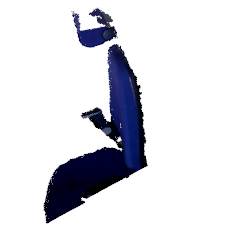
\includegraphics[width=0.30\textwidth]{images/annotations/original/chair1_front_ut}}
%   \subfloat[chair2]{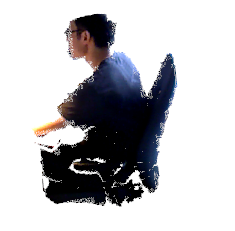
\includegraphics[width=0.30\textwidth]{images/annotations/original/chair2_front_ut}}
%   \caption{Selection of objects from the dataset.}
%   \label{fig:objects_ut}
% \end{figure}

\section{Downsampling}
In their merged forms, the clouds on average contain approximately 4,300,000
points for a room which is around 4m wide, 5.5m deep and 3m high. This number of
points does not actually provide us with much additional information, since the
intermediate frames all have the same resolution. As such, we can safely
downsample the cloud to get a more reasonable number of points.

To downsample, we make use of a voxel grid, which splits the 3D space in which
the cloud sits into smaller subspaces of equal size called voxels. The width,
height and depth of voxels in the space can be specified, but we are interested
in keeping all dimensions the same resolution, and so we specify the parameters
so that each voxel is a cube. At this stage, we would like to perform a simple
downsampling to reduce the number of points, but we wish to keep small details
in the cloud --- something in the realm of a 1cm resolution is ideal in this
case.

Downsampling with a 1cm resolution gives a reduction in size of the clouds of on
average 78\%, to approximately 950,000 points.
Figure~\ref{fig:downsample_effect} shows the effect of the downsampling. While
there is slight degradation of the textures, this is to some extent a visual
effect which is viewpoint dependent. Most of the structure in the cloud is
retained, which is key. This step is important, as it greatly affects the speed
of computation of subsequent steps in the system, but it is a trade off. If the
downsampling resolution is too low, then we lose a lot of information about the
surface structure of parts of the cloud. This is likely to lead to worse
performance when trying to find matches. How tolerant we are to low resolution
also depends on the kinds of objects that we are interested in finding. If we do
not care about smaller objects, then even with a lower resolution the results
should still be satisfactory. However, a lower resolution likely means that it
will be necessary to look at larger regions of space in order to describe
points. We will investigate the effects of this in appendix~\ref{chap:exp}.

\begin{figure}
  \centering
  \centerline{
    \subfloat[Sofa]{
      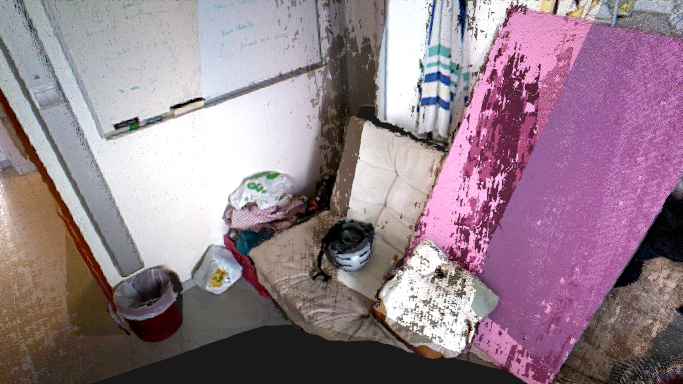
\includegraphics[width=0.60\textwidth]{images/sofa_og}
      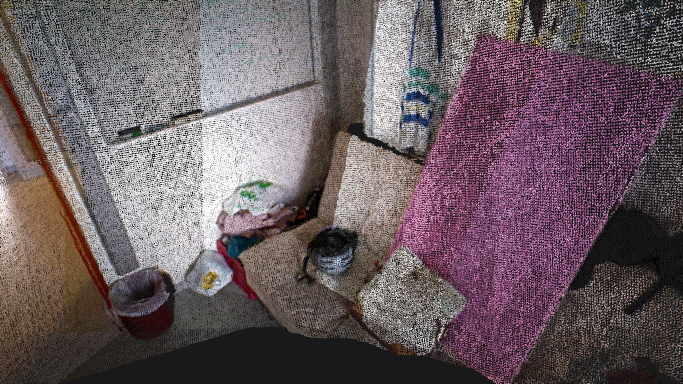
\includegraphics[width=0.60\textwidth]{images/sofa_ds}
    }\\
  }
  \centerline{
    \subfloat[Desk 1]{
      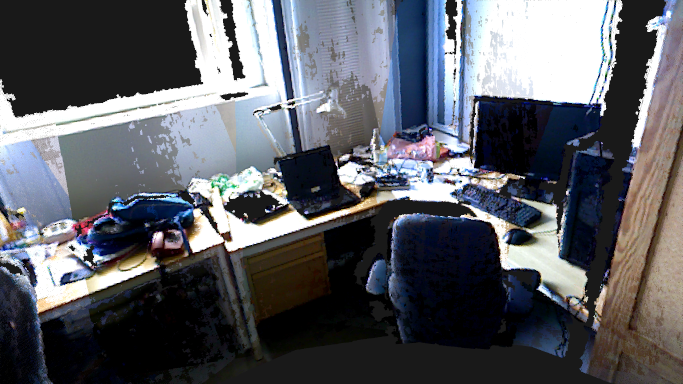
\includegraphics[width=0.60\textwidth]{images/johan_og}
      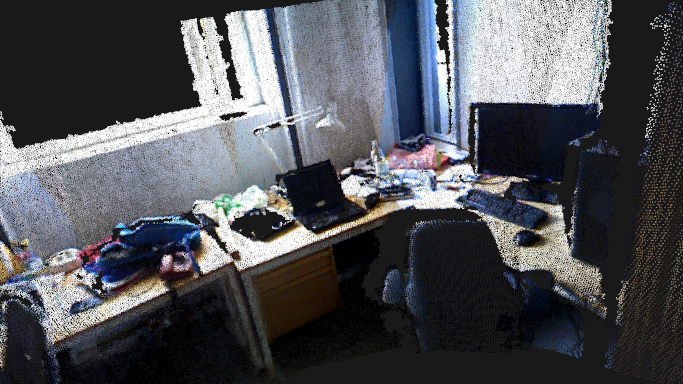
\includegraphics[width=0.60\textwidth]{images/johan_ds}
    }\\
  }
  \centerline{
    \subfloat[Desk 2 side]{
      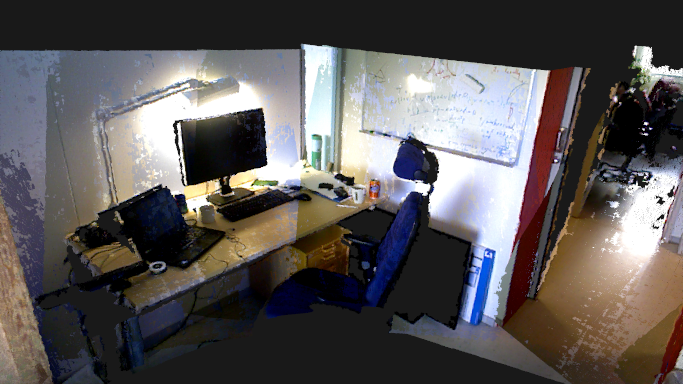
\includegraphics[width=0.60\textwidth]{images/nils_side_og}
      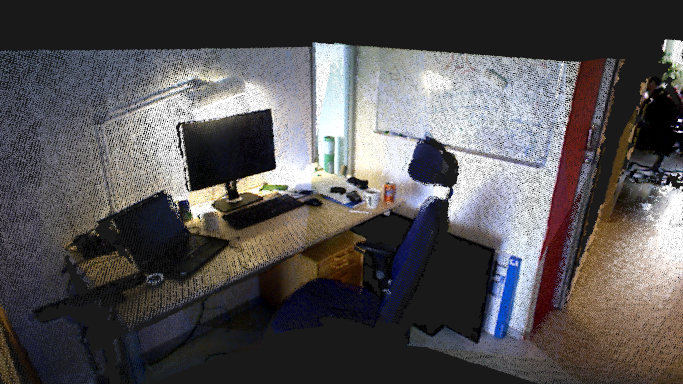
\includegraphics[width=0.60\textwidth]{images/nils_side_ds}
    }\\
  }
  \centerline{
    \subfloat[Desk 2 front]{
      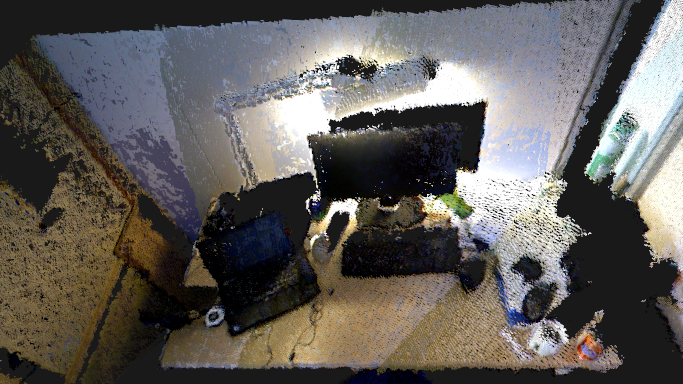
\includegraphics[width=0.60\textwidth]{images/nils_front_og}
      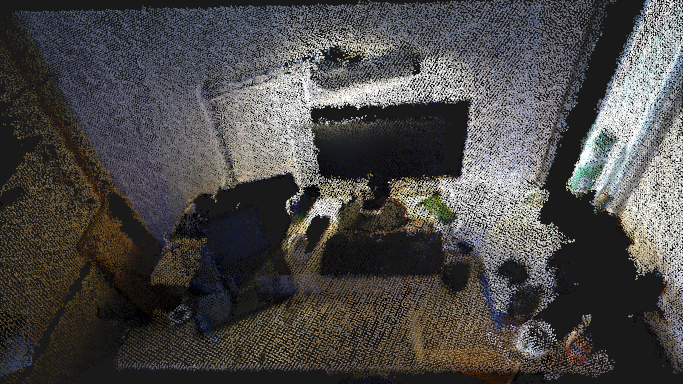
\includegraphics[width=0.60\textwidth]{images/nils_front_ds}
    }\\
  }
  \caption{The effect of downsampling. The left column shows the original
    clouds, the right column clouds downsampled with voxel size of 1cm$^3$.}
  \label{fig:downsample_effect}
\end{figure}

\section{Transformation and Trimming}
\begin{figure}[t]
  \centering
  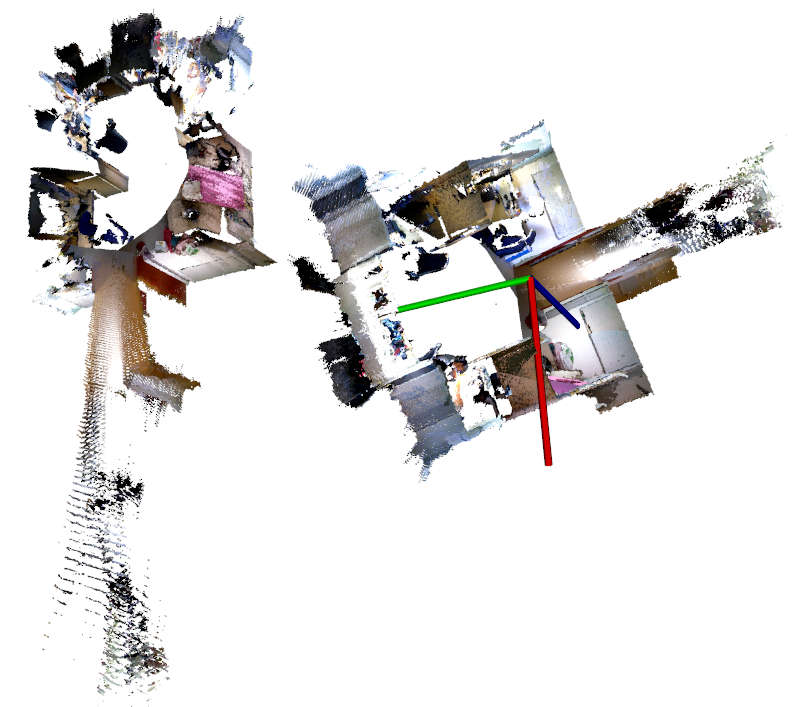
\includegraphics[width=0.8\textwidth]{images/orig_transformed}
  \caption{Original cloud and the transformed cloud. The original cloud is on
    the left, transformed on the right. The coordinate axis shows the global
    reference frame --- none of the axes are aligned for the original cloud, but
    the transformed cloud is well aligned with the $x$-$y$ plane (green and red lines).}
  \label{fig:orig_transformed}
\end{figure}

Once the cloud has been downsampled, there is a little more that needs to be
done in order to get the cloud into a convenient form. The raw data that we have
has clouds which have their origin at the position of the camera while the room
was being scanned. Our data is a subset of a larger dataset which contains
clouds of more than one room --- if we were to use the data without applying any
additional transformations, all the clouds would sit on top of each other at the
origin, whereas we would ideally like to have them in their true position
relative to the origin. The robot collecting data knows its position, so this
information is stored.

As mentioned before, each cloud is a combination of a number of intermediate
frames, each of which has corresponding information about the pose of the camera
when the frame was taken, which we can use to transform the complete cloud into
its actual position in space.

An added benefit of this transformation is that it allows us to remove the floor
and ceiling by using a simple thresholding filter on the $z$ axis, as the floor
of the cloud is now aligned with the $x$-$y$ plane of the global reference
frame, as opposed to being aligned with the cloud's rotated reference frame
(Figure~\ref{fig:orig_transformed}) The threshold for the ceiling can be
determined by measuring the ceiling height, and the floor is assumed to be a
$z=0$. We add a small offset to each of the values to ensure that the parts are
correctly removed even if there is some noise.

Although we would like the system to be as generic as possible, the particular
subset of clouds that we are using have a large number of points outside the
room which do not give any useful information. To this end, we also include
additional filters on the $x$ axis to remove these points.
Figure~\ref{fig:trimmed} shows the end result of this step.

\begin{figure}
  \centering
  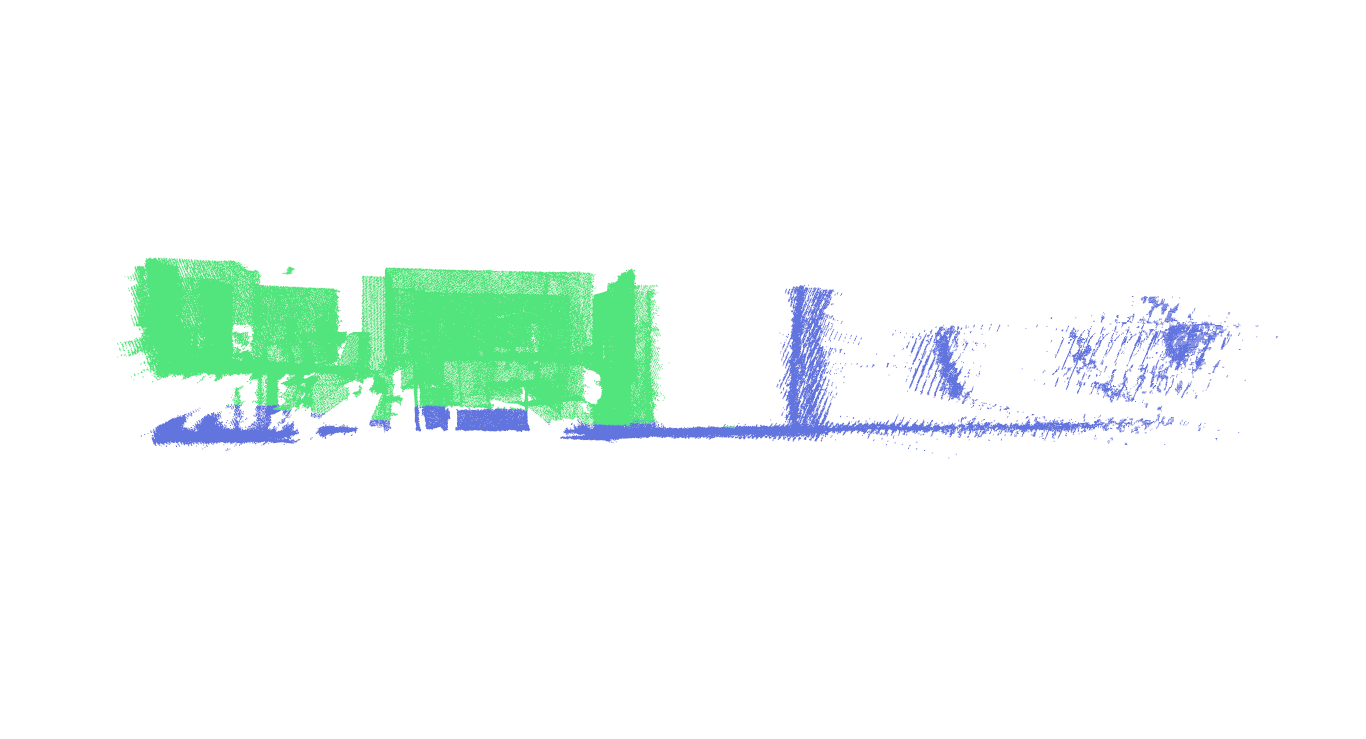
\includegraphics[width=0.9\textwidth]{images/trimmed_side}
  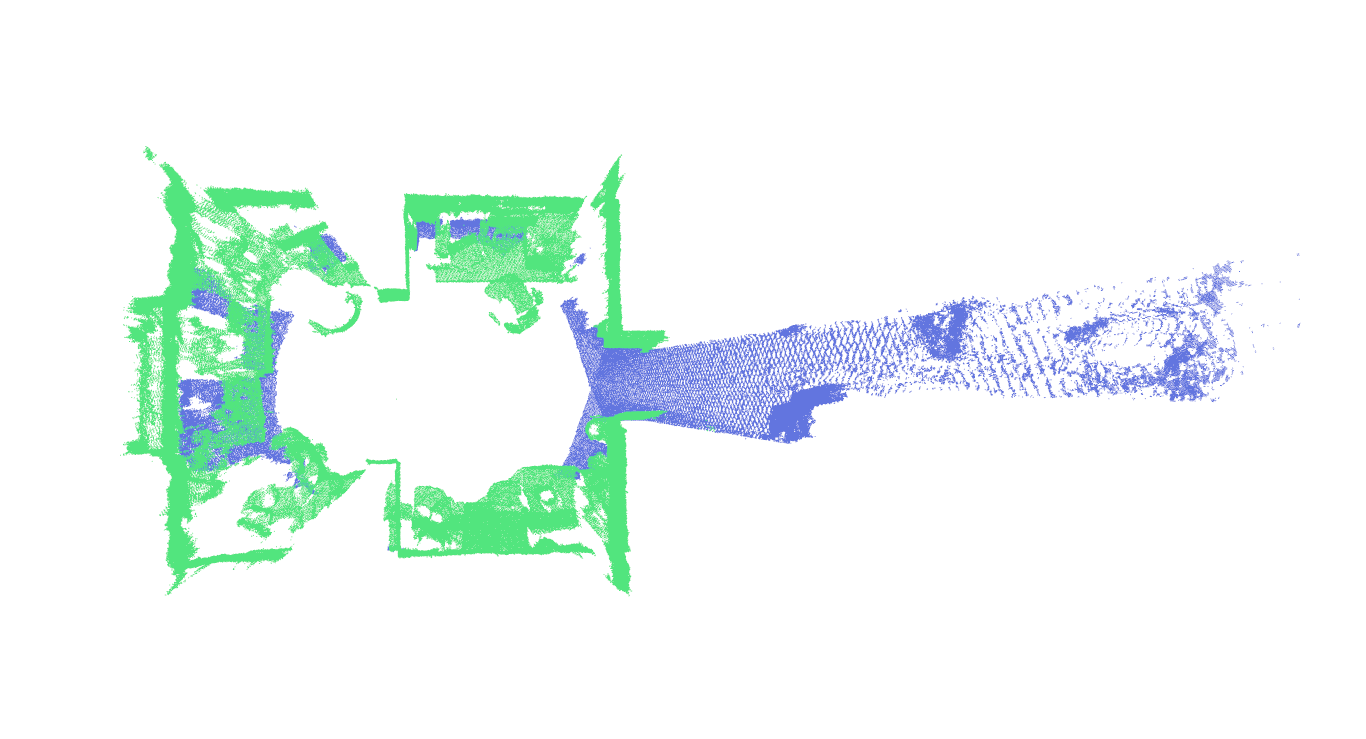
\includegraphics[width=0.9\textwidth]{images/trimmed_top}
  \includegraphics[width=0.9\textwidth]{images/trimmed_diag_left}
  \includegraphics[width=0.9\textwidth]{images/trimmed_diag_right}
  \caption{Result of trimming step. Transformed cloud is blue, trimmed is green.}
  \label{fig:trimmed}
\end{figure}

\section{Plane Extraction}
Having extracted normals from the cloud, we come to what is the most costly
preprocessing step. Due to the structured nature of our dataset, the number of
planes present in the clouds is quite high. While the presence of planes can be
used to define surfaces and the like, in our system we are not interested in
using the planes for anything in particular, and as such removing them from the
cloud is good, because we remove a large portion of points in the clouds which
are not be parts of any object, speeding up computation time of subsequent
steps.

Plane extraction is done by running RANSAC multiple times with a plane model. A
plane can be described by its general form equation
\begin{equation}
  \label{eq:1}
  ax+by+cz+d=0\,,
\end{equation}
where the normal vector $\mathbf{n}$ is defined by the coefficients $a$, $b$ and
$c$. To get the model coefficients, RANSAC samples three points ($p_1,p_2$ and
$p_3$) from the input cloud. From these three points, the normal is computed
using the cross product \cite{planeeq}

\begin{equation}
  \label{eq:2}
  \mathbf{n}=(p_2-p_1)\times(p_3-p_1)\,.
\end{equation}

Once the plane coefficients have been computed, we must find the inlier points of this
plane model, based on their distance to the plane. The perpendicular distance of
a point $p$ to a plane is
\begin{equation}
  \label{eq:3}
  D=\frac{\mathbf{n}\cdot p + d}{\mid \mathbf{n} \mid}\,.
\end{equation}

A point is considered to be an inlier if $D<D_t$, where $D_t$ is some threshold
on the distance. The RANSAC algorithm repeats the point sampling $n$ times,
storing the plane coefficients and number of inliers. At the end of the process,
the best plane the one with the largest number of inliers.

While this simple formulation can work well, there can be issues where the
planes that are extracted are not actually planes, due to there being regions in
the cloud where there can be a large number of inliers, but no actual plane, as
seen in Figure~\ref{fig:planenormal}. This effect can be mitigated by including
a single additional step to the inlier check, which also looks at the angle
between the plane normal and the normal at the point, computed by
\begin{equation}
  \label{eq:5}
  \theta=\cos^{-1}(\mathbf{n}\cdot p)\,.
\end{equation}

A point is then considered an inlier only if it passes the distance threshold
check and $\theta<\theta_t$, where $\theta_t$ is the threshold on the angle.
This simple addition gives much more consistent results.

The RANSAC implementation that we are working with uses only a single distance
computation
\begin{equation}
  \label{eq:6}
  D_a=(1-p_c)w_n\theta + (1-((1-p_c)w_n))D\,,
\end{equation}
where $p_c$ is the curvature at the point $p$, and $w_n$ is a predefined weight
on the distance between the point and plane normals. $p_c\rightarrow 0$ on flat
surfaces, so in these regions the normal will have a higher influence on the
aggregate distance $D_a$, whereas in regions of high curvature the euclidean
distance will be more important. Inliers are points where $D_a<T$.

When extracting planes, we use several parameters in addition to the aggregate
distance threshold $T$ to tweak the behaviour. The main aim of the additional
parameters is to prevent planes which are too small from being extracted. We
set a hard limit on the total number of planes which can be extracted, and also
define a threshold on the minimum number of points $N_{\min}$ in a plane.
\begin{equation}
  \label{eq:7}
  N_{\min}=\max(\eta N_{\text{trim}},\, N_{\text{fixed}})\,,
\end{equation}
where $\eta$ is a small positive positive value. Since we are dealing with large
clouds, a suitable range of values is $\left[0.02,0.05\right]$.
$N_{\text{trim}}$ is the number of points in the trimmed cloud.
$N_{\text{fixed}}$ is a fixed value. We choose the maximum of the two values to
ensure that fluctuations in the cloud size are compensated for.
\newpage
\begin{figure}[H]
  \centering
  \includegraphics[width=0.49\textwidth]{images/normals_comb}
  \caption{Example of the smoothing effect of normal estimation radius. From
    bottom to top, 0.01, 0.025, 0.5, 0.2, 0.25, 0.5cm radius. Normals are
    indicated by orange lines. Note the tendency of normals with higher radius
    to tilt as they approach the corner. Normals on the top section are slightly
    skewed due to perspective.}
  \label{fig:normal_corner}
\end{figure}


\begin{figure}[H]
  \centering
  \subfloat[Plane model]{\includegraphics[width=0.49\textwidth]{images/plane_nonorm}}
  \subfloat[Plane-normal model]{\includegraphics[width=0.49\textwidth]{images/plane_withnorm}}
  \caption{RANSAC with basic plane model and with plane-normal model. Notice the
    horizontal planes extracted in the basic model, and the extraction of the
    couch in the bottom left which is not very plane-like.}
  \label{fig:planenormal}
\end{figure}
\section{Normal Estimation}
In this step, normals are estimated for each point in the cloud. The normal at a
point is the vector which is perpendicular to the curvature of the surface at
that point. By estimating normals for clouds, we can get some more information
about the surface structure of the cloud. Normals are used in several parts of
the system, including by feature selection methods and features. As mentioned
above, they are also used in the plane extraction step to increase accuracy.

There are many ways of estimating normals, but the method we use is formulated
as a least squares plane fitting problem, which is used to estimate the normal
of the plane tangent to the surface at the point at which the normal is to be
computed \cite{RusuDoctoralDissertation}. The computation gives an ambiguous
result in terms of the sign of the normal. To correct for this, a viewpoint is
needed, which serves to define what sign is used. Perhaps the most important
thing to note is that the normal must be computed using points in a
neighbourhood; either within a certain radius, or the nearest $k$ points. The
neighbourhood determines the scale factor that results. A small neighbourhood
gives a small scale factor, and a large neighbourhood a large scale factor. A
large scale factor can be bad if the objects that one is trying to examine have
regions where the rate of change of surface curvature is high, such as at the
corners of tables. It results in the smearing of edges and the suppression of
fine detail \cite{RusuDoctoralDissertation}. Figure~\ref{fig:normal_corner}
shows an example of the effect of different neighbourhood sizes on the results.

\begin{figure}
  \centering
  \subfloat[0.02m]{\includegraphics[width=0.49\textwidth]{images/plane_normal_0,02}}
  \subfloat[0.04m]{\includegraphics[width=0.49\textwidth]{images/plane_normal_0,04}}\\
  \subfloat[0.06m]{\includegraphics[width=0.49\textwidth]{images/plane_normal_0,06}}
  \subfloat[0.08m]{\includegraphics[width=0.49\textwidth]{images/plane_withnorm}}
  \caption{Planes extracted with different settings for the normal radius.
    Notice in particular the improved extraction of the back wall as normal
    radius increases.}
  \label{fig:plane_normrad}
\end{figure}

During preprocessing we compute two different sets of normals using different
settings for the radius. One set is for use with plane extraction, which has a
higher value for the radius, somewhat mitigating the effect of noise on the
normals, and resulting in less patchy extraction of planes
(Figure~\ref{fig:plane_normrad}).
\chapter{Interest Point Selection}
\label{chap:interest}
Once the preprocessing step has been completed, we can move on to computing
features from the processed clouds. First, however, we need to choose the points
at which the descriptors will be computed. The idea of interest point selection
is to choose points in the cloud which are better in some way than other points
for feature extraction --- which points these are depends on the method used.
This is important, as if we can compute descriptors at locations which are
unique to an object, it makes any correspondences that are found when comparing
the descriptors likely to be actual occurrences of the object in the clouds in
which we are searching.

In this section we will describe in some detail the methods that we use. The
interest point selection methods and descriptors are implemented in the Point
Cloud Library\cite{pcl}, an open source library for point cloud manipulation and
processing.

\section{Uniform}
The first and most obvious method of selecting points for feature extraction is
not to try to select interesting points at all, but to simply spread points
uniformly over the space. With this method, one would expect to extract a larger
number of points than with targeted methods (depending on the spread of points
used), and since the entire space is covered, it is unlikely that there will be
any omissions of points that are interesting.

The problem with having a large number of points is that this results in more
features having to be computed and compared in later stages.

To compute the uniform points, we simply downsample the cloud once more. The
size of the voxels used determines the spread of the points over the space ---
the behaviour of this method is determined entirely by a single parameter.
\section{ISS}
Zhong~\cite{zhong2009intrinsic} introduces the Intrinsic Shape Signature (ISS)
interest point selection method as one of a series of steps in the computation
of the ISS descriptor introduced in the same paper.

The main component of this method is the scatter matrix, which is the covariance
matrix of points within a spherical region around a sample point. For a point
$p_i$, the $3\times 3$ scatter matrix is
\begin{equation}
  \label{eq:4}
  S(p_i)=\sum_{\mid p_j - p_i \mid < r_s}(p_j-p_i)(p_j-p_i)^T\,,
\end{equation}
where $p_j$ is another point in the cloud. $r_s$ defines the saliency radius,
which limits the points which we consider to be in the neighbourhood of $p_i$.
Interest points are only extracted in regions where there are at least $n_{min}$
points in the neighbourhood of $p_i$.

Once $S$ is computed, its eigenvalues $\lambda^1_i, \lambda^2_i$ and
$\lambda^3_i$ (with decreasing magnitude) are extracted. The smallest eigenvalue
$\lambda^3_i$ can be used to measure the 3D point variations in the
neighbourhood of the point \cite{zhong2009intrinsic}. If it happens that two of
the eigenvalues computed are equal, the reference frame of the point can become
ambiguous, so limits are applied to the ratio of the eigenvalues such that
\begin{equation}
  \label{eq:8}
  \frac{\lambda^2_i}{\lambda^1_i}< \gamma_{21},\, \frac{\lambda^3_i}{\lambda^2_i}< \gamma_{32}\,.
\end{equation}

With this formulation, it is likely that more points are considered interest
points than are not. To thin the interest points further, non-maximum
suppression is used. Essentially, this removes from the interest points any
point where the value of $\lambda^3_i$ at the point is not the maximum in the
neighbourhood of the point. This neighbourhood is defined by the radius $r_{n}$,
whose value is usually distinct from the value of $r_s$.
\section{SUSAN}
The SUSAN (Smallest Univalue Segment Assimilating Nucleus) detector is based on
an algorithm introduced for 2D feature detection by Smith~\cite{smith1997susan}.
We use an extension of this detector to 3D. The basis for the SUSAN principle
comes from the concept of each image point having an associated local area which
has intensity and normal direction values that are similar to it.

A spherical region called the mask is defined, with some radius $r_m$ which has
at its centre a point referred to as the nucleus. Looking at the points within
the spherical region, we compare their values of the normal direction and
intensity to the nucleus values. From this comparison, a region of space which
has similar values to the nucleus can be defined. This region is known as the
univalue segment assimilating nucleus or USAN. Figure~\ref{fig:susan_nucleus}
shows this principle in the 2D case. The USAN contains information about the
structure of the cloud in small region. Depending on the position of the nucleus
in the cloud, the volume of the USAN will vary. In regions where all points are
similar, the USAN is large, and it is small when the region has a large
variation in point intensity and normal direction. Based on this observation,
using the inverted USAN volume as a feature detector should result in the
selection of descriptive points --- hence the name \emph{Smallest} USAN.

\begin{figure}
  \centering
  \includegraphics[width=0.48\textwidth]{images/susan1}
  \includegraphics[width=0.48\textwidth]{images/susan}
  \caption{Concept of nucleus and mask in 2D SUSAN detector. USAN is the white
    region in the right image \cite{zhang2013susan}.}
  \label{fig:susan_nucleus}
\end{figure}

To compute SUSAN keypoints, the following process is applied to each point $p_i$
in the cloud. First, all points $p_j$ in the neighbourhood defined by $r_m$ are
found. We then define the USAN and the centroid of the mask. In order to be
considered as part of the USAN, a point must fulfill the inequalities
\begin{align}
  \label{eq:9}
  \left|I_i-I_j\right|&\leq I_t\\
  1-\mathbf{n}_i\cdot\mathbf{n}_j&\leq \theta_t\,,
\end{align}
where $I$ is the intensity of a point, and $\mathbf{n}$ is the normal, and $I_t$
and $\theta_t$ are user-defined thresholds on the intensity and angular
difference. The intensity is computed from RGB values using
\begin{equation}
  \label{eq:10}
  I=\frac{r+g+b}{3}\,.
\end{equation}

We assume that each channel of the RGB value of a point has the same weight.

The centroid $C$ is computed using
\begin{equation}
  \label{eq:11}
  C=\frac{1}{\left|\text{USAN}\right|}\sum_{p_j \in \text{USAN}}p_j\,.
\end{equation}

The last thing to do for each point is to ensure that the number of points in
the USAN is within the bound
\begin{equation}
  \label{eq:13}
  0 < \left| USAN \right| < 0.5(N-1)\,,
\end{equation}
where $N$ is the number of points in the neighbourhood of the nucleus. If this
check is successful, the output intensity of the nucleus is set to
$I_o=0.5(N-1)-\left|USAN\right|$. This defines the response of the feature
selection at this nucleus.

% Some additional validation can also be applied to the
% point, checking that the distance $\mid\mid p_i-C\mid\mid<d_t$, where $d_t$ is a
% user-defined threshold on the distance. 
% If either the geometric threshold check or nucleus check fail, the point is
% not included in the interest point set.

Once $I_o$ has been computed for all valid points in the cloud, non-maximum
suppression is applied. Only those points which have the minimal intensity in
the neighbourhood defined by $r_m$ are used as the final interest points.

\section{SIFT}
The Scale Invariant Feature Transform (SIFT), introduced by
Lowe~\cite{lowe2004distinctive} in 1999, it is still commonly used for many 2D
image processing applications. The most important concept introduced in the
paper is that of scale invariance --- the SIFT feature extraction method
automatically selects features at different scales. This effect is achieved by
applying a Gaussian blur with different standard deviation in 2D, and by
downsampling clouds in 3D. The leaf size used for downsampling is determined by
the number of \emph{octaves} $N_o$. Within each octave, there are several
\emph{scales} $N_s$ which are applied. After all scales in an octave have been
computed, the leaf size is doubled, and the process repeated, until it has been
applied to all octaves.

For each octave, the procedure begins with downsampling the point cloud to the
scale defined for that octave $S_{o}$, which initially is set to the minimum
scale $S_{\min}$. The scales in the octave are then defined by
\begin{equation}
  \label{eq:14}
  s_i=\frac{S_o\cdot 2^{i - 1}}{N_s}\,,
\end{equation}
where $0<i<N_s$. Each point $p$ in the cloud has its nearest neighbours $P_{nn}$ computed,
within a radius three times the maximum scale $s_{N_s}$ in that octave. The same
neighbours are used for computation of the difference of Gaussians $D$ for each
scale in the octave. In each scale, a Gaussian response $R$ is computed
\begin{equation}
  \label{eq:15}
  R_i=\frac{\sum_{q\in P_{nn}}0.299q_r + 0.587q_g +
    0.114q_b\exp\left\{-\frac{0.5}{\sigma}\mid\mid p-q\mid\mid\right\}}{\sum_{q\in P_{nn}}\exp\left\{-\frac{0.5}{\sigma}\mid\mid p-q\mid\mid\right\}}\,,
\end{equation}
where $q_r$, $q_g$ and $q_b$ are the red, blue and green channels of the colour at the
point $q$, $\sigma=s_i^2$. The difference of Gaussians is then
\begin{equation}
  \label{eq:16}
  \text{DoG}_i=R_i-R_{i-1}\,,
\end{equation}
where $1<i<N_s$. These values are then used to find extrema in the scale space.
The neighbourhood of each point is examined again, and the maximum and minimum
values of the DoG at any point within the neighbourhood are found for each
scale. For consideration as an interest point, the value of DoG$_i$ must be
greater than a minimum contrast threshold $t_c$. This limits the inclusion of
points where the responses are not very different. If this threshold is
exceeded, the value of DoG at the point is checked to see if it is a maximum or
a minimum in its neighbourhood, and is either larger or smaller than the maximum
and minimum values for the same point in the neighbouring scale spaces. If all
these criteria are fulfilled, the point is added to the interest points.

Once this process is completed for a single octave, the scale $S_o$ is doubled,
and the process repeats $N_o$ times. The selected interest points are the
aggregated results from each individual octave. 

\section{Harris}
Like SIFT, the Harris detector, introduced by the eponymous
Harris~\cite{harris1988combined}, was originally used as a method for edge and
corner detection in images. Much like ISS, it uses a covariance matrix applied
to the neighbourhood of a point as the basis of its function. Rather than using
the points themselves, however, the Harris detector finds the covariance matrix
of the normals in the neighbourhood. The response at the point is then computed
by combining the determinant and trace of the matrix. The resulting responses
for each point are then thinned using non-maximum suppression, and the remaining
points are the interest points.

\begin{figure}
  \centering
  \subfloat[Uniform]{\includegraphics[width=0.49\textwidth]{images/uniform_points}}
  \subfloat[ISS]{\includegraphics[width=0.49\textwidth]{images/iss_points}}\\
  \subfloat[SUSAN]{\includegraphics[width=0.49\textwidth]{images/susan_points}}
  \subfloat[SIFT]{\includegraphics[width=0.49\textwidth]{images/sift_points}}
  \caption{Examples of results of different plane extraction methods.}
  \label{fig:planemethod}
\end{figure}
\chapter{Descriptor Extraction}
\label{chap:descriptors}
In this step, we compute descriptors at each of the locations that was selected
by the interest point method that was used. The end goal of the combination of
the interest point selection and descriptor extraction steps is to produce a set
of descriptors that can be used to represent the scene without having to keep
all of the original data. In addition, putting information about the scene into
a compact representation also allows the comparison of two scenes much more
quickly than would otherwise be possible. Instead of comparing complex
structures in the scene, simple vectorial representations are compared instead.
The intention is to compute these representations and have them stored, so that
they can be accessed later to compare to the descriptors extracted from query
objects. Correspondences between descriptors from the query object and parts of
the room clouds should indicate the presence of the object in that cloud. We
will try to use this to more reliably retrieve objects.

However, finding a compact representation that is also distinctive enough and
produces similar results for similar regions of space is not easy. In the image
processing literature, a lot of work has been done to develop novel descriptors
which are faster to compute, are invariant to more effects that might reduce
their effectiveness, and better represent the image data. As with interest point
selection methods, current methods in 3D often make use of the lessons learned
from the development of 2D methods. 

\section{SHOT}
\begin{figure}
  \centering
  \includegraphics[width=\textwidth]{images/shotcolor}
  \caption{Representation of the construction of the SHOTCOLOR descriptor and
    the subdivisions used for local histogram computation.}
  \label{fig:shotcolor}
\end{figure}
The Signature of Histograms of OrienTations (SHOT) descriptor is the product of
a study on 2D descriptors, particularly SIFT, and makes extensive use of
histograms, as the authors believe that this is part of the reason why the
descriptor is so effective \cite{tombari2010unique}. The paper also discusses
the importance of the local reference frame, or RF. Defining a local RF is a way
to ensure that the same descriptor will be computed if the same points are
translated or rotated, or if there is noise or clutter in the region the
descriptor algorithm uses to define the descriptor values. This is analogous to
the problem of rotation and scale invariance in 2D descriptors. The RF is
computed based on the eigenvalue decomposition of a special scatter matrix $M$
\begin{equation}
  \label{eq:12}
  M=\frac{1}{\sum_{i:d_i\leq R}(R-d_i)}\sum_{i:d_i\leq R}(R-d_i)(\mathbf{p}_i-\mathbf{p})(\mathbf{p}_i-\mathbf{p})^T\,,
\end{equation}
where $R$ is the radius used to define the neighbourhood used to compute the
descriptor, $\mathbf{p}$ is the point at which the feature is to be computed,
$\mathbf{p}_i$ is another point in the cloud, and $d_i$ is the Euclidean
distance between $\mathbf{p}_i$ and $\mathbf{p}$.

The addition made by the authors to previous work is to use a weighted linear
combination, where the weight of a point is lower the further it is from the
central point. This is in order to reduce the effect of clutter. The eigenvalue
decomposition alone is not sufficient to define an unambiguous RF. To do so, the
authors use a technique introduced in \cite{bro2008resolving}, which orients the
signs of the eigenvectors to make them coherent with those of the points that
they are representing.

Having defined the local RF, information about the location of points within $R$
is accumulated to create the descriptor. This is done by computing local
histograms within subdivisions of the spherical region, and then grouping them
together to form the final descriptor. The spherical region is split into 32
regions by splitting the sphere along the radial, azimuth and elevation axes, as
seen in Figure~\ref{fig:shotcolor}. Points in each subdivision are grouped into
bins of the local histogram according to the cosine of the angle between their
normals and the normal of the feature point $\mathbf{p}$. This formulation
reduces computation time, and does not require complicated binning. Using the
actual angle to allocate points to bins has the disadvantage of needing
different bin resolutions depending on whether directions are close to or
orthogonal to the normal direction \cite{tombari2010unique}.

\section{SHOTCOLOR}
In a subsequent paper, the authors of SHOT introduce an extension to the
descriptor which also includes colour information \cite{tombari2011combined}. To
include colour information, the same histogramming method is applied, but
instead of using the dot product of the RGB vectors at the feature point and a
neighbourhood point, the authors use the $L_1$ norm of the RGB value converted
to the CIELab colour space. The value a pair of points is therefore
\begin{equation}
  \label{eq:17}
  l(C_p, C_q)=\sum^3_{i=1}\mid C_p(i)-C_q(i)\mid\,,
\end{equation}
where $C$ is the CIELab colour triple of a point.

\section{USC}
Another descriptor introduced by Tombari is the Universal Shape Context (USC)
\cite{tombari2010uniquesc}. This descriptor is an improvement of the 3D shape
context, in the sense that it has a unique reference frame, constructed in the
same way as for SHOT. As with SHOT, a spherical region is defined by a radius
$R_s$ and a central point, and separated into a number of bins. For each point,
the number of points $N$ in a local region defined by radius $R_d$ is computed.
A weighting $w$ for this point is then computed according to
\begin{equation}
  \label{eq:18}
  w=\frac{1}{N}V_b\,,
\end{equation}
where $V_b$ is the volume of the bin that the point falls within. For each
point, $w$ is accumulated in the descriptor vector according to the bin into
which it falls. The final descriptor is therefore a representation of the
combined weights of all of the points in the sphere.
\section{PFH}
\begin{figure}
  \centering
  \includegraphics[width=0.48\textwidth]{images/darboux}
  \caption{Darboux frame defined by the vectors $u$, $v$ and $w$ \cite{rusu2008learning}.}
  \label{fig:darboux}
\end{figure}
The Point Feature Histogram (PFH) is the first in a family of descriptors
described by Rusu et al. \cite{rusu2008aligning}. The descriptor was developed
in order to improve performance of cloud matching with iterative closest point
(ICP). Most of the descriptors used for that purpose previously had only a
single dimension, and as a result could not be properly descriptive over a whole
scene. The descriptor is likely to have a similar value at different points in
the scene, which causes problems as one cannot have a high confidence that a
correspondence between two points in two different scenes is the correct one.

To solve this problem, the PFH descriptor uses a vector rather than a scalar
value, computed based on histograms, which allows for more distinctive features.
As with all other descriptors, operations are done on points within a radius $r$
of the central point $p$. Each pair of points in the neighbourhood is examined,
as in Figure~\ref{fig:pfhinfluence}. In each pair, a source point $p_s$ and a
target point $p_t$ are determined by looking at the normals of the points, and
comparing the angles relative to the line connecting the two points. The point
whose normal has the smaller angle is the source, the other the target. A
reference frame with the origin as the source point is defined using the normal
of the source $n_s$ as
\begin{align}
  \label{eq:19}
  u&=n_s\\
  v&=(p_t-p_s)\times u\\
  w&=u\times v\,,
\end{align}
as shown in Figure~\ref{fig:darboux}.

Using this frame, four features are computed
\begin{align}
  \label{eq:20}
  f_0&=v\cdot n_t\\
  f_1&=\mid\mid p_t - p_s\mid\mid\\
  f_2&=\frac{u\cdot(p_t-p_s)}{f_1}\\
  f_3&=atan(w\cdot n_t,u\cdot n_t)\,,
\end{align}
where $n_t$ is the normal of the target point. These values are then used to
compute an index
\begin{equation}
  \label{eq:21}
  idx=\sum^3_{i=0}\left\lfloor \frac{f_i\cdot d}{f_{i\max}-f_{i\min}}\right\rfloor\cdot d^i\,,
\end{equation}
that defines which of the histogram bins the pair of points falls. $d$ is the
number of divisions to apply to the possible feature value range
$f_{i\max}-f_{i\min}$. The value of $d$ defines the dimensionality of the final
descriptor --- the higher its value the larger the number of bins in the
histogram. The bins in the histogram start zeroed, and are incremented by a
value based on the number of points in the descriptor region each time the
value from Equation~\eqref{eq:21} is the index of that bin.

Because this descriptor computation operates on \emph{all} point pairs in the
neighbourhood, depending on the size of the neighbourhood and the point density,
computation can be slow.
\begin{figure}
  \centering
  \subfloat[PFH]{\includegraphics[width=0.48\textwidth]{images/pfh}}
  \subfloat[FPFH]{\includegraphics[width=0.48\textwidth]{images/fpfh}}
  \caption{Influence diagrams of the PFH and FPFH descriptors \cite{rusu2009fast}.}
  \label{fig:pfhinfluence}
\end{figure}
\section{FPFH}
The Fast Point Feature Histogram (FPFH) was introduced to tailor the PFH
descriptor to real time applications while maintaining its discriminative power
\cite{rusu2009fast}. Instead of computing the values in Equation~\eqref{eq:19}
for every pair of points in the neighbourhood of $r$, they are only computed for
each point and its $k$ neighbours $p_k$ within the same radius --- this is
called the simplified point feature histogram (SPFH). Because of the use of two
neighbourhoods, the final descriptor can include information from points up to
$2r$ away. Once the SPFH value for each point in the neighbourhood is computed,
it is integrated into the final FPFH descriptor using
\begin{equation}
  \label{eq:20}
  FPFH(p)=SPFH(p)+\frac{1}{k}\sum^k_{i=1}\frac{1}{\omega_k}\cdot SPFH(p_k)\,,
\end{equation}
where $k$ is the number of neighbours within $r$ and $\omega_k$ is the distance
between $p$ and $p_k$.

Because only direct neighbours of each point are considered, some
interconnections that would exist in the PFH computation do not in FPFH, which
contributes to its increased speed. The downside of this is that some of the
geometric structures which exist in the region will not be included. In
addition, due to the nature of the computation, the values for some points will
be factored into the descriptor twice.

A further improvement made by the authors is a modification of the way the
histogram is populated. Instead of using \eqref{eq:21} to index into
an array where a single index indicates certain value ranges for all the
features, they use separate histograms for each feature and concatenate them.
In the original case, there might be a large number of indices which do not
contain any information, because combined feature values do not fall into the
ranges. In the simplified case, there are likely to be fewer histogram indices
which do not contain any information.
\section{PFHRGB}
An extension of the original PFH descriptor, this version also takes into
account RGB values of points when computing features. This adds three features
to the four from \eqref{eq:20}. The computation is simple, taking the
ratio of colour values between the two points $p_s$ and $p_t$ and ensuring that
they are in the interval $\left[-1,1\right]$.
\begin{align}
  \label{eq:22}
  f_4=\frac{p_{s_r}}{p_{t_r}}\\
  f_5=\frac{p_{s_g}}{p_{t_g}}\\
  f_6=\frac{p_{s_b}}{p_{t_b}}\,.
\end{align}

If one of the values $f_i$ is outside the interval, then it is pushed back into
the interval using
\begin{equation}
  \label{eq:23}
  f_i=-\frac{1}{f_i}\,.
\end{equation}

These values are then added to the histogram and combined to create the final
descriptor as with the basic PFH method.

\chapter{Object Query}
\label{chap:query}
The final step in the system is to use the features that have been extracted
from the original clouds, and from those clouds retrieve what we think is likely
to be the object that we are looking for. It is necessary to mention here the
assumption we make about objects received by the system. That is, we assume the
cloud that makes up the object consists of points that come only from that
object and nothing else. Or, to look at this from the opposite perspective, we
assume that the entirety of the cloud received by the system is the object.

This assumption changes the problem somewhat. Since our basic assumption from
the beginning is that we do not have any labelled in the system, it would be
much more complex for the system to receive, for example, a single frame from
a scan of a room. In order to perform object query in this scenario, it would be
necessary to have a definition of ``objectness'', which could facilitate the
segmentation of the frame into objects and non-objects. These segmented objects
could then be used effectively for object query as the cloud would actually be
representative of that object.

\section{Preprocessing Objects}
To ensure that the objects are in a usable form, we apply the downsampling,
transformation and normal extraction steps from Chapter~\ref{chap:preprocess}.
Without downsampling the feature extraction step is particularly expensive,
because there are a large number of points concentrated in small regions, so
even with a small radius, the number of neighbours that have to be examined is
generally very large. In addition, the raw annotations have issues with a
``slicing'' effect caused by the positioning of the camera when the frames were
taken, and its depth resolution (Figure~\ref{fig:slicing}). Using the raw clouds
to compute features would most likely result in worse retrieval performance as
the surface structure of the cloud is essentially a series of stacked planes,
which is not actually what the surface looks like in the target clouds that we
are passing to the system.

\begin{figure}
  \centering
  \subfloat[Chair]{
    \begin{tabular}{c}
      \includegraphics[width=0.2\textwidth]{images/annotations/slices/chair_front}\\
      \includegraphics[width=0.2\textwidth]{images/annotations/slices/chair_side}
    \end{tabular}
  }
  \subfloat[Backpack]{
    \begin{tabular}{c}
      \includegraphics[width=0.2\textwidth]{images/annotations/slices/backpack_front}\\
      \includegraphics[width=0.2\textwidth]{images/annotations/slices/backpack_side}
    \end{tabular}
  }
  \subfloat[Jacket]{
    \begin{tabular}{c}
      \includegraphics[width=0.2\textwidth]{images/annotations/slices/hanger_jacket_front}\\
      \includegraphics[width=0.2\textwidth]{images/annotations/slices/hanger_jacket_side}
    \end{tabular}
  }
  \subfloat[Trash bin]{
    \begin{tabular}{c}
      \includegraphics[width=0.2\textwidth]{images/annotations/slices/trash_bin_front}\\
      \includegraphics[width=0.2\textwidth]{images/annotations/slices/trash_bin_side}
    \end{tabular}
  }
  \caption{Slicing effect on unprocessed annotation clouds. With a slight
    rotation, an initially complete-looking cloud shows its
    flaws.}
  \label{fig:slicing}
\end{figure}

\section{Query Process}

The query systemn receives two clouds; the query cloud, containing the features
extracted from the cloud of the object that we are interested in finding, and
the target cloud, which contains features extracted from the cloud which we wish
to search for the object. For point $q$ in the query cloud, we search the target
cloud for the closest $K$ points using a nearest neighbour search. As we do not
care about the exact distance, but only the relative distances of points, we use
a simplified $L_2$ norm which does not take the square root of distances,
returning only the sum of the squares of the differences between each dimension,
which speeds up computation. The nearest neighbour search uses optimised
functions implemented in the FLANN library \cite{muja2009fast,
  muja2014scalable}.

In the next step, we make use of the computed nearest neighbours of each point
to place votes into a 3D grid overlaid onto the target cloud. We construct the
grid with a width, depth and height based on the minimum and maximum values of
the $x$, $y$ and $z$ dimensions of the points in the target cloud. This space is
then subdivided using a step, which defines the dimensions of each of the
individual voting cells. For each neighbour descriptor, we add a vote in the
grid in the cell that contains the point at which it was computed.

This voting scheme is more robust than simply taking the single nearest
descriptor. In some cases there will be locations where the descriptor matches
some other point in the space better than the actual corresponding point on the
object we are interested in finding. By taking a number of nearest neighbours
and using all of them to vote, we hope to populate the voting space in such a
way that these false positive values are hidden by the true positives, leading
to a space where the position of the actual object is the one where there is the
highest concentration of votes. We would expect this to be the case, as while
some of the descriptors will match other positions in the cloud, the majority
are likely to be found in regions where the actual object is.


\begin{algorithm}
  \DontPrintSemicolon
  \SetKwInput{Kw}{Init}
  \KwData{$k$-d tree representation of cloud $P$, Empty cluster list $C$, empty queue $Q$, processed point list $L$}
  \For{$p_i\in P,\, p_i \notin L$}{
    $Q \longleftarrow p_i$\;
    \For{$q_i\in Q$}{
      Find set $P^j_k$ of neighbours $p_j$ of $q_i$ where $q_i - p_j < r$
      \For{$p^j_k\in P^j_k$}{
        \If{$p^j_k \notin L$}{
          $Q \longleftarrow p^j_k$\;
          $L \longleftarrow p^j_k$\;
        }
      }
    }
    $C \longleftarrow Q$\;
    $Q \longleftarrow \emptyset$\;
  }
  \caption{Euclidean Cluster Extraction \cite{RusuDoctoralDissertation}}
  \label{alg:euc}
\end{algorithm}

Once the voting grid is populated, we perform clustering in this space to
extract regions which contain potential matches. The clustering performed is
simple Euclidean clustering, shown in Algorithm~\ref{alg:euc}. The voting grid
consists of cells in 3D space, and we represent each cell by a point at its
centre. During the voting process, there will be many points which do not
receive any votes, and these points are not interesting to us, so we exclude
them from the point cloud generated from the voting space. Rather than using all
of the points with a non-zero number of votes, we extract the top $N$ points
ranked according to the number of votes. If, as we would hope, most of the
points with high numbers of votes correspond to the query object, then they are
likely to be in the same spatial region, and can therefore be extracted by the
clustering. The clustering works by adding an initial seed point to a queue, and
adding points within radius $r$ of that point in the queue. The original point
is then added to a ``processed'' queue and will not be considered in any other
clusters. The rest of the points in the queue are processed in the same way,
adding points within radius $r$ of those points. Once there are no more points
which are within the radius of any point in the queue, the queue is converted to
a cluster. The process then begins again with another point from the cloud which
is not already part of a cluster. The clustering does not take into account the
number of votes a point has when checking its neighbours. If no clusters are
found, then we use the point in the voting space which has the highest number of
votes as a cluster of a single point.

\begin{figure}
  % 20140905/patrol_run_29/room_2/
  \centering
  \subfloat[Voting]{\includegraphics[width=0.8\textwidth]{images/votes_shotc}}\\
  \subfloat[Clustering]{\includegraphics[width=0.8\textwidth]{images/clusters_shotc}}
  \caption{Examples of voting and clustering using the SHOTCOLOR feature and
    uniform sampling with a radius of 0.2 and 5 neighbours. The query object is
    an example of the chair on the right. Large points in the voting show points
    belonging to the top $N$ points. Points are coloured according to the number
    of votes they have. The clusters are coloured by rank from red to green,
    blue and yellow.}
  \label{fig:clusters_ex}
\end{figure}

\begin{figure}
  \centering
  \centerline{
    \subfloat[334 points]{\includegraphics[width=0.2\textwidth]{images/region_0}}
    \subfloat[251 points]{\includegraphics[width=0.2\textwidth]{images/region_1}}
    \subfloat[186 points]{\includegraphics[width=0.2\textwidth]{images/region_2}}
    \subfloat[169 points]{\includegraphics[width=0.2\textwidth]{images/region_3}}
  }\\
  \centerline{
    \subfloat[138 points]{\includegraphics[width=0.2\textwidth]{images/region_4}}
    \subfloat[118 points]{\includegraphics[width=0.2\textwidth]{images/region_5}}
    \subfloat[75 points]{\includegraphics[width=0.2\textwidth]{images/region_6}}
  }
  \caption{Regions extracted based on centroids of clusters found in
    Figure~\ref{fig:clusters_ex}.}
  \label{fig:cluster_regions}
\end{figure}

Once points have been clustered, the total score of each cluster is computed by
summing the votes of all the points it contains. Once this is done, we rank the
clusters by their scores. In this action, we make the assumption that the larger
the score, the higher chance that the cluster lies on the object. Another option
is to also consider the point density by dividing the score by the total number
of points in the cluster. For each cluster, we find its centroid and then remove
a sphere with a radius of $\alpha r$ centred on this point from the target
cloud. $\alpha$ is a small multiplier greater than 1, used to ensure that a
large part of the object is captured even if the centroid is offset from the
object. This extracted region should contain the object.
Figure~\ref{fig:clusters_ex} shows an example of the votes and clusters
extracted using the procedure. Figure~\ref{fig:cluster_regions} shows the
corresponding regions extracted from the target cloud, of which three are
instances of the query object.

\chapter{Conclusion and Further Work}
\label{chap:conc}
In this report, we have presented our implementation of a system for object
query in point clouds. We use a query cloud which contains points from a single
object to search in target clouds. The first step in our system is to preprocess
the clouds to remove points which do not contribute any useful information to
the query system, such as planes. For this process, we used RANSAC, along with
downsampling and some additional trimming and transformation. In the second step
of the process, we select interesting points using one of several possible
methods, and then extract descriptors at these locations. In the final step, the
descriptors are compared to descriptors of the same type from a given query
cloud. U using a voting scheme in 3D space along with clustering, we extract
regions in which we believe the query object appears in the target cloud.

In our experimental evaluation (Appendix~\ref{chap:exp}), we discovered that the
system had an optimal retrieval rate of approximately 50\% of the actual number
of objects of a given instance in the target cloud. This value was achieved only
for the chair object, which appears to have some unique regions that the
descriptor comparisons can pick up more frequently than for other objects. The
backpack object had retrieval rates of around 40\%, while the rates for other
objects were much lower, around 10-15\%. We also found that in terms of interest
point selection, the best methods to use were uniform and ISS, which return a
large number of points. We believe that these methods perform best due to the
large numbers of points resulting in more points from the object being included
in the voting space, and contributing to the cluster scores. The best performing
descriptor was PFHRGB, followed by SHOTCOLOR, both of which include colour
information in addition to shape, which is the main difference between these two
descriptors and the others that we have used. The PFHRGB descriptor outperforms
SHOTCOLOR in most cases, which we believe to be the result of the PFH family
being more descriptive of the shape. However, in our evaluation of the
descriptor computation times, PFHRGB was the most costly to compute, so there is
a trade-off that can be made if faster operation is necessary. We found that
keeping a larger number of the nearest neighbours of the query descriptor from
the target cloud gave better results, presumably because the more descriptors
from the object can contribute to the voting space and increase the likelihood
of a cluster forming. An increase of the total number of points used when
clustering also improved results.

While the system works satisfactorily for two of the objects we used for
testing, the results do not look particularly good in the general scheme of
things. A 50\% retrieval rate is less than one would like, but considering that
we have done only the bare minimum of preprocessing and descriptor computations,
the results could be seen as favourable. We have skipped some expensive
segmentation steps which might seek to separate objects from the scene before
doing any computations. We use basic nearest neighbour matching to retrieve the
closest descriptors to a query descriptor, and then use a simple clustering
technique to select the points that we are interested in.

\section{Possible Improvements}
The system has many areas which could be improved, in particular in terms of
computation time. The RANSAC plane extraction is very expensive, and as a result
preprocessing takes a long time. There are still regions which are useless after
the preprocessing step has completed, so there is room for faster methods, and
those which remove more points which we do not wish to keep. Due to time
constraints, we have been unable to do a thorough investigation of the effects
of various parameters on the efficacy of the retrieval, especially for the
descriptors and interest point selection methods. The parameters for the
preprocessing generally work quite well, but as mentioned above there is room
for improvement.

Some improvements to the query stage are also likely to improve the retrieval
rate. We had considered investigating the effect of applying a density estimate
to the voting space and using that as a search space instead of just points in
space, but we did not have enough time to try this approach --- it would be
interesting to see what difference this would make to the output of the system.
Another possibility which is similar to a density estimate would be to vary the
clustering radius for each point based on its vote count; points with higher
values would have a larger radius. This could have a positive effect on the
clustering, as it would ensure that points with high number of votes have larger
clusters. It might also mitigate some of the issues with pruning of small
clusters if the maximum point happens to be in a relatively sparse region of
space. It is difficult to speculate on the exact effect that this would have. 

In terms of general usability, the system would benefit from an interface which
would allow the user to more easily input a query object and receive results
once processing is complete. This addition could include a learning system which
would ask the user to select matches of the actual object out of the matches
that were returned, and use these results to improve subsequent searches by
weighting the descriptors in the regions from which the user-selected matches
came from, and considering these weights when voting.

\appendix
\chapter{Experimental Results}
\label{chap:exp}
In this chapter, we will investigate the effects of different variables or
descriptors on the output of different parts of the system. We will also look at
the computation time of the various parts of each step. In addition, we will
attempt to discuss the reasons for the variations that we observe. The goal of
this section is to give the reader an insight into the behaviour of the system
under different parameter settings, and more importantly, to present retrieval
results from our data set.

The data that we have consists of 86 clouds of the same room, at different times
over the period of approximately a month. Each cloud also has some annotated
objects in the form of clouds which have the object segmented from the scene.
Each object has a corresponding label so that it can be identified in any of the
clouds.

All experiments were run on a Lenovo X230 with 16GB of RAM and an 2.90GHz Intel
i7-3520M processor. The machine was in use throughout the time of the
experiments, so there is likely to be some variation introduced into the
computation time due to other processes.

\section{Preprocessing}
Although each stage in the system is important, the preprocessing step has a
large impact on the performance of the system in later stages. In particular,
the number of points removed from a cloud can affect the results both positively
and negatively, the plane extraction in particular. If tuned correctly, it can
remove most of the extraneous planes, leaving only parts of the scene which have
some non-planar structure, which are most likely to be objects. 

Several settings affect the result of preprocessing. The distance threshold $d$
defines the threshold below which points are considered to be part of the plane
model. The distance is computed according to \eqref{eq:6}. Another
important parameter that affects RANSAC directly is the number of iterations
$N$. Because of the random sampling, it is possible to be unlucky with the point
selections made, so retrying only a few times can result in the planes that are
extracted having only a small number of points on them. However, the process of
recomputing the distances to all points takes a long time, so if $N$ is too
high, the time cost might outweigh the improved results. $M$ is the maximum
number of planes that are to be extracted from a cloud. We set a hard limit
$P_{\min}$ on the minimum number of points in a plane. If an extracted plane has
fewer than $P_{\min}$ points, it is discarded and RANSAC is rerun. The number of
times that the system will skip a plane is also fixed. If too many planes are
skipped, the extraction procedure will exit.

We also define parameters for the normal computations. The radius $n_p$ is used
when computing normals for planes, and $n_f$ is used when extracting normals for
features. During development we noticed that a higher radius on the plane
extraction normals generally led to better results in terms of the number of
points removed by the procedure. In contrast, for feature normals we would like
to try to retain smaller details about the surfaces, so a smaller radius makes
more sense in order to avoid smoothing effects.

The final parameter that is used is the leaf size $l$ for downsampling, which
determines the dimensions of the voxels.

\subsection{Parameter Settings}
We have used several different parameter settings for testing. We will refer to
them using the shortened keys below.

\begin{description}
\item[DEF] This indicates the base parameter setting from which we make changes.
  The settings here were determined through observation of performance during
  development.
  \begin{itemize}
  \item $d=0.05$
  \item $N=300$
  \item $M=10$
  \item $P_{\min}=20000$
  \item $n_p=0.08$
  \item $n_f=0.03$
  \item $l=0.01$
  \end{itemize}
\item[DT] Reduced distance threshold for RANSAC, reduced value for the
  minimum number of points.
  \begin{itemize}
  \item $d=0.02$
  \item $P_{\min}=8000$
  \end{itemize}
\item[NR] Reduced plane normal computation radius
  \begin{itemize}
  \item $n_p=0.04$
  \end{itemize}
\item[RI500] Increased RANSAC iterations
  \begin{itemize}
  \item $N=500$
  \end{itemize}
\item[RI100] Decreased RANSAC iterations
  \begin{itemize}
  \item $N=100$
  \end{itemize}
\item[RI50] Decreased RANSAC iterations
  \begin{itemize}
  \item $N=50$
  \end{itemize}
\item[DS15] Increased downsample leafsize
  \begin{itemize}
  \item $l=0.015$
  \end{itemize}
\item[DS15M] Increased downsample leafsize, decreased minimum points
  \begin{itemize}
  \item $l=0.015$
  \item $P_{\min}=9000$
  \end{itemize}
\item[DS2] Increased downsample leafsize
  \begin{itemize}
  \item $l=0.02$
  \end{itemize}
\item[DS2M] Increased downsample leafsize, decreased minimum points
  \begin{itemize}
  \item $l=0.02$
  \item $P_{\min}=4500$
  \end{itemize}
\end{description}
\subsection{Analysis}
\begin{table}
  \centerline{
    \begin{tabular}{r|llllllll}
      Setting & Downsample & Trim & Normals & Planes & PerPlane &  NormalsF & Total \\\hline
      DEF & 0.72$\pm$0.08 & 0.16$\pm$0.06 & 16.33$\pm$1.11 & 116.12$\pm$13.63 & 15.10$\pm$1.43 & 1.42$\pm$0.21  & 133.32$\pm$14.13 \\
      DT & 0.54$\pm$0.06 & 0.23$\pm$0.02 & 12.29$\pm$1.30 & 114.30$\pm$18.81 & 13.69$\pm$1.65 & 1.65$\pm$0.17 & 127.35$\pm$19.44 \\
      NR & 0.88$\pm$0.35 & 0.18$\pm$0.08 & 4.12$\pm$0.54 & 175.35$\pm$35.32 & 26.31$\pm$5.32 & 1.60$\pm$0.27  & 180.52$\pm$35.44 \\
      RI500 & 1.07$\pm$0.22 & 1.82$\pm$0.81 & 13.20$\pm$1.23 & 262.81$\pm$60.10 & 34.19$\pm$9.00 & 1.17$\pm$0.20 & 278.90$\pm$60.37 \\
      RI100 & 1.14$\pm$0.38 & 1.25$\pm$1.63 & 14.92$\pm$6.96 & 62.68$\pm$21.67 & 10.59$\pm$3.78 & 1.86$\pm$0.99  & 80.00$\pm$24.77 \\
      RI50 & 0.70$\pm$0.09 & 0.17$\pm$0.06 & 15.86$\pm$0.99 & 16.02$\pm$5.02 & 3.82$\pm$1.02 & 2.15$\pm$0.48  & 32.75$\pm$5.30 \\                                          
      DS15 & 0.99$\pm$0.23 & 0.10$\pm$0.03 & 3.65$\pm$0.52 & 51.43$\pm$17.19 & 12.47$\pm$4.93 & 0.65$\pm$0.15  & 56.17$\pm$17.27 \\
      DS15M & 0.87$\pm$0.31 & 0.34$\pm$0.50 & 4.77$\pm$2.27 & 100.47$\pm$116.74 & 13.05$\pm$16.78 &0.68$\pm$0.29 & 106.45$\pm$116.80 \\
      DS2 & 0.58$\pm$0.07 & 0.03$\pm$0.00 & 1.31$\pm$0.14 & 13.32$\pm$2.06 & 7.71$\pm$1.56 & 0.41$\pm$0.06  & 15.24$\pm$2.08 \\
      DS2M & 0.56$\pm$0.10 & 0.03$\pm$0.00 & 1.23$\pm$0.25 & 32.13$\pm$4.06 & 4.26$\pm$0.61 & 0.23$\pm$0.05 & 33.96$\pm$4.27 \\
    \end{tabular}
  }
  \caption{Average time taken in seconds for various stages of preprocessing. The total
    time is a sum of downsample, trim, normals and planes, skipping the feature
    normal computation. Average over 86 clouds. ($\mu\pm\sigma$)}
  \label{tbl:preprocess_time}

  \centerline{
    \begin{tabular}{r|llllll}
      Setting & Original & Downsampled & Trimmed & NPlanes & PerPlane & Planes \\\hline
      DEF & 4,347,665$\pm$125,147 & 988,703$\pm$40,359 & 783,173$\pm$34,610 & 7.78$\pm$1.30 & 50,542$\pm$6,301 & 394,992$\pm$46,514\\
      DT & \ditto & \ditto &  \ditto & 8.42$\pm$1.87 & 20,114$\pm$2,382 & 615,910$\pm$40,667 \\
      NR & \ditto & \ditto & \ditto & 6.75$\pm$1.03 & 44,261$\pm$4,269 & 508,862$\pm$48,995 \\
      RI500 & \ditto & \ditto & \ditto & 7.74$\pm$1.10 & 52,250$\pm$6,407 & 386,967$\pm$39,903 \\
      RI100 & \ditto & \ditto & \ditto & 6.22$\pm$1.85 & 45,224$\pm$9,510 & 519,703$\pm$102,722 \\
      RI50 & \ditto & \ditto & \ditto & 4.60$\pm$2.32 & 38,566$\pm$15,670 & 583,620$\pm$115,296 \\
      DS15 & \ditto & 485,732$\pm$20,386 & 368,765$\pm$16,645 & 4.42$\pm$1.53 & 26,500$\pm$4,772 & 248,010$\pm$45,101 \\
      DS15M & \ditto & \ditto & \ditto & 7.90$\pm$1.20 & 22,657$\pm$3,172 & 192,516$\pm$16,784 \\
      DS2 & \ditto & 276,378$\pm$11,503 & 203,385$\pm$8,910 & 1.58$\pm$0.94 & 10,766$\pm$6,312 & 180,607$\pm$17,235 \\
      DS2M & \ditto & \ditto & \ditto & 7.84$\pm$1.29 & 12,001$\pm$1,505 & 110,543$\pm$12,245
    \end{tabular}
  }
  \caption{Number of points in various stages of preprocessing, taken as an
    average over 86 clouds. NPlanes indicates the number of planes extracted.
    PerPlane is the number of points per plane, computed from the number of
    planes and the difference in number of points between Trimmed and Planes.
    Average over 86 clouds. ($\mu\pm\sigma$)}
  \label{tbl:preprocess_num}
  \centering
  \begin{tabular}{r|ccccc}
    Setting & Downsample & Trim & Trim Orig & Plane & Plane Orig \\\hline
    DEF & 0.23$\pm$0.01 & 0.79$\pm$0.01 & 0.18$\pm$0.00 & 0.50$\pm$0.06 & 0.09$\pm$0.01 \\ 
    DT & \ditto & \ditto & \ditto & 0.79$\pm$0.04 & 0.14$\pm$0.01 \\ 
    NR & \ditto & \ditto & \ditto & 0.63$\pm$0.05 & 0.12$\pm$0.01 \\
    RI500 & \ditto & \ditto & \ditto & 0.49$\pm$0.05 & 0.09$\pm$0.01 \\ 
    RI100 & \ditto & \ditto & \ditto & 0.65$\pm$0.12 & 0.12$\pm$0.02 \\ 
    RI50 & \ditto & \ditto & \ditto & 0.75$\pm$0.15 & 0.13$\pm$0.03 \\
    DS15 & 0.11$\pm$0.00 & 0.76$\pm$0.02 & 0.08$\pm$0.00 & 0.67$\pm$0.12 & 0.06$\pm$0.01 \\
    DS15M & \ditto & \ditto & \ditto & 0.52$\pm$0.04 & 0.04$\pm$0.00 \\ 
    DS2 & 0.06$\pm$0.00 & 0.74$\pm$0.02 & 0.05$\pm$0.00 & 0.89$\pm$0.07 & 0.04$\pm$0.00 \\
    DS2M & \ditto & \ditto & \ditto & 0.54$\pm$0.06 & 0.03$\pm$0.00
  \end{tabular}
  \caption{Reduction of point numbers as proportion of cloud size at previous step
    (columns 1,2 and 4) and original cloud (columns 3 and 5), as an
    average over 86 clouds. ($\mu\pm\sigma$)}
  \label{tbl:time_reduction}
\end{table}

\begin{figure}
  % cloud from 20140901/patrol_run_33/room_1
  \centering
  \centerline{
    \subfloat[DEF]{\includegraphics[width=0.45\textwidth]{images/exp_planes_def}}
    \subfloat[DT]{\includegraphics[width=0.45\textwidth]{images/exp_planes_dt}}
    \subfloat[NR]{\includegraphics[width=0.45\textwidth]{images/exp_planes_nr}}\\
  }
  \centerline{
    \subfloat[RI500]{\includegraphics[width=0.45\textwidth]{images/exp_planes_ri500}}
    \subfloat[RI100]{\includegraphics[width=0.45\textwidth]{images/exp_planes_ri100}}
    \subfloat[RI50]{\includegraphics[width=0.45\textwidth]{images/exp_planes_ri50}}\\
  }
  \centerline{
    \subfloat[DS15]{\includegraphics[width=0.45\textwidth]{images/exp_planes_ds15}}
    \subfloat[DS15M]{\includegraphics[width=0.45\textwidth]{images/exp_planes_ds15m}}
    \subfloat[DS2M]{\includegraphics[width=0.45\textwidth]{images/exp_planes_ds2m}}
  }
  \caption{Comparison of the result of plane extraction on the same arbitrarily
    chosen cloud for different parameter settings. Green regions are extracted
    planes, blue regions are the remaining cloud which is output by the
    preprocessing step. DS2 result not shown as no planes were extracted.}
  \label{fig:ransaciter}
\end{figure}

Table~\ref{tbl:preprocess_time} shows the time taken by various stages of
preprocessing. As is clear from the table, and as expected, the majority of the
time is spent on RANSAC, for plane extraction. The second most costly operation
is the normal computation. From
Tables~\ref{tbl:preprocess_num}~and~\ref{tbl:time_reduction}, we can see that
the largest reduction in points occurs in the downsampling step, as expected.
The trimming and plane extraction also reduce the clouds by a large proportion,
but the number in terms of raw points is much smaller due to the downsampling.

Looking at the timings for the decreased distance threshold (DT), we see that
they are almost the same as the default setting, as we would expect. However,
even though DT extracts more planes, likely as a result of the reduced minimum
number of points, the size of the clouds at the end of the process is
approximately 1.3 times the size of those produced by the default setting. This
is because the number of inlier points on each plane is greatly reduced by the
limit on the distance. In general the smaller distance threshold results in
fewer points being removed from the clouds.

The NR set has a normal computation time that is much faster than those of other
settings with the same downsampling size. This is because the number of points
used to compute the normal at each point is smaller, and as a result the
computation of the plane parallel to the normal is faster. Although NR performs
better in terms of reduction than DT, it is still not as good as the default
setting from that perspective. This is because the smaller normal radius results
in less smoothing, which means that points which are actually on planes may have
noise on the normals which result in them not being added. While the NR set
should have timings for planes similar to DEF and DT, the plane computation time
seems to have increased a lot. We do not have a satisfactory explanation for
this --- we ran a second shorter experiment to check the timings, and the
results were similar. This is an unexpected result as the number of planes
extracted on average is also very similar. Furthermore, the internal
computations done by RANSAC should not be affected, since the same number of
normals must be compared in each case. We are unable to determine the reason
behind this effect.

The RI sets look at the effect of the RANSAC iterations, and as expected it is
very noticeable. RI500 has a much increased computation time due to the
increased iterations, but the reduction that results is not much better than the
result using only 300 iterations in the DEF set. We can see that increasing the
number of iterations has diminishing returns in terms of the increased number of
points removed versus the additional computation time. Decreasing the number of
iterations has the opposite effect --- reducing computation time, but also
reducing the number of points removed.

In the DS sets, we look at the effect of the leaf size used for downsampling.
Increasing the leaf size greatly reduces the number of points in the cloud, as
is to be expected. This also affects subsequent steps, as both normal
computation and RANSAC examine fewer points. In terms of the proportion of
points removed, for DS15 and DS2 we did not reduce the minimum points per plane,
and this effect shows in the results. Fewer planes were removed, and as a
consequence the effectiveness of the plane extraction is reduced. In the DS2M
and DS15M sets, we decrease the minimum points per plane, and the proportions
are more in line with what would be expected, extracting proportionally almost
as many points as that extracted by the default setting.

Figure~\ref{fig:ransaciter} shows examples of planes extracted using the
different parameter settings, and the clouds that go on to the next stage of processing.

\section{Descriptor Extraction and Interest Point Selection}
As mentioned before, the descriptor extraction and interest point selection steps
are important for the effectiveness of queries, in terms of selecting points
that are on the object in the cloud that we are interested in searching.
An evaluation of the retrieval process can be found in Section~\ref{queryexp}.
In this section we will mention the parameter settings for the various methods,
and do a simple analysis of the results of our experiments.

\subsection{Parameter Settings}
\subsubsection{Interest Point Selection}
Since all of the selection methods use a radius value for computation in some
way or another, we have selected values that are similar for all of the methods.
During some preliminary evaluations, we also attempted to use the Harris method,
but we received anomalous values from it and decided to drop it from further
testing.
\begin{description}
\item[Uniform] Uniform feature selection has only a single parameter; the
  downsample leaf size $l$. This setting varies the number of points selected,
  and their locations, but in a much more structured way than the other methods.
  For the experiments we have set $l=0.05$.
\item[ISS] For this method, we have set the saliency radius $r_s=6R$, where $R$
  is the resolution of the cloud. The resolution is simply the average squared
  distance between points in the cloud. The non-maximum suppression radius
  $r_n=4R$ --- we check to see if this point is non-maximum in a smaller
  region than is used to contribute to the computation of the point's value. The
  minimum number of points $n_{\min}$ for non-maximum suppression is set to 5.
  The eigenvalue thresholds $\gamma_{21}=\gamma_{32}=0.975$. This setting is
  based off the default value in PCL.
\item[SUSAN] The mask and non-maximum suppression radius $r_m=0.05$. The
  intensity threshold $I_t=7$, and the threshold on the angle between normals is
  $\theta_t=0.001$. These latter values are also based on the default found in
  PCL.
\item[SIFT] For SIFT, we have set the minimum scale $S_{\min}$ to 0.04, with 4
  octaves $o$ and 5 octave scales $o_s$. The minimum contrast has been set to
  zero, so we retain all features.
\end{description}

\subsubsection{Descriptor Extraction}
For our experiments we have used the SHOT, SHOTCOLOR, PFH, FPFH and PFHRGB
methods. We decided not to use the USC descriptor as in preliminary evaluations
the time required for comparing large numbers of the descriptors was high.

The descriptor extraction methods all have only a single setting, which is their
radius. We have decided to use a radius of 0.05m for our experiments. The
objects that we have selected are large enough that this radius should give a
good description of interesting regions, without losing too much of the fine
detail.

\newpage
\section{Analysis}
\begin{figure}
  \centering
  \centerline{
    \subfloat[DEF, $N=18076$]{\includegraphics[width=0.4\textwidth]{images/int/uniform_0_05}}
    \subfloat[$l=0.08,\, N=7340$]{\includegraphics[width=0.4\textwidth]{images/int/uniform_0_08}}\\
  }
  \centerline{
    \subfloat[$l=0.1,\, N=4765$]{\includegraphics[width=0.4\textwidth]{images/int/uniform_0_1}}
    \subfloat[$l=0.12,\, N=1360$]{\includegraphics[width=0.4\textwidth]{images/int/uniform_0_12}}
  }
  \caption{Interest points extracted using uniform method with various voxel
    dimensions. $N$ indicates the number of points in the cloud.}
  \label{fig:intuni}
\end{figure}

Figure~\ref{fig:intuni} shows the interest points extracted with the uniform
method, with different settings for the voxel dimension parameter. As is to be
expected, the whole space is covered uniformly with points in all cases. Note
how points which are mostly surrounded by empty space remain in the interest
points even through the higher values of the parameter. While these loner points
generally appear with other methods, there is usually a way to remove such
points from contention, in particular using non-maximum suppression or nearest
neighbour checks. We have decided to set the default value to give quite a large
number of points, as we believe that the only way the uniform method can be
viable is if there are a large number of descriptors on the object that can be
matched.

\begin{figure}
  \centering
  \centerline{
    \subfloat[DEF, $N=6956$]{\includegraphics[width=0.45\textwidth]{images/int/iss_def}}
    \subfloat[$n_{\min}=12,\, N=6310$]{\includegraphics[width=0.45\textwidth]{images/int/iss_def_minn12}}
    \subfloat[$r_s=12R$, $N=6126$]{\includegraphics[width=0.45\textwidth]{images/int/iss_sal12}}\\
  }
  \centerline{
    \subfloat[$r_s=12R,\, r_n=8R,\, N=1345$]{\includegraphics[width=0.45\textwidth]{images/int/iss_sal12_nm8}}
    \subfloat[$r_s=12R,\, r_n=8R,\, n_{\min}=10,\, N=1293$]{\includegraphics[width=0.45\textwidth]{images/int/iss_sal12_nm8_minn10}}
    \subfloat[$r_s=4R,\, n_{\min}=2,\, N=30966$]{\includegraphics[width=0.45\textwidth]{images/int/iss_sal4_nm2} \label{subf:salnm2}}
  }
  \caption{Interest points extracted using ISS for various parameter settings.
    $N$ indicates the number of points in the cloud. Values not shown in
    captions are set to the same values as DEF.}
  \label{fig:intiss}
\end{figure}

The ISS extraction results (Figure~\ref{fig:intiss}) look quite similar to those
of the uniform method, but on closer inspection one can see that more points
have been removed, due to non-maximum suppression. With $n_{\min}=12$, we can
see that some of the loner points that appear, for example in the right hand
side of the cloud, have been removed. Adjusting this parameter upwards will tend
to reduce the number of points in the cloud, while reducing it will tend to
increase the number of points, or rather, reduce the number of points that are
removed due to not being close to enough other points. Increasing $r_s$ also
slightly reduces the number of points, most likely due to the additional points
considered in the covariance matrix. The largest reduction in point density can
be achieved by adjusting $r_n$, since this parameter defines the radius within
which a point must have the maximal third eigenvalue. If the values are set too
low, then a very large number of points are extracted. In the case of
Figure~\ref{subf:salnm2}, the neighbour minimum has been set too low and far too
many points are retained.

\begin{figure}
  \centering
  \centerline{
    \subfloat[DEF, $N=3058$]{\includegraphics[width=0.45\textwidth]{images/int/susan_r0_05}}
    \subfloat[$\theta_t=0.05,\, N=2487$]{\includegraphics[width=0.45\textwidth]{images/int/susan_r0_05_at0_05}}
    \subfloat[$\theta_t=0.1,\, N=2106$]{\includegraphics[width=0.45\textwidth]{images/int/susan_r0_05_at0_1}}\\
  }
  \centerline{
    % \subfloat[$\theta_t=1$]{\includegraphics[width=0.45\textwidth]{images/int/susan_r0_05_at1}}
    \subfloat[$I_t=30,\, N=2032$]{\includegraphics[width=0.45\textwidth]{images/int/susan_r0_05_it30}}
    \subfloat[$r_m=0.08,\, N=1217$]{\includegraphics[width=0.45\textwidth]{images/int/susan_r0_08}}
    \subfloat[$r_m=0.1,\, N=791$]{\includegraphics[width=0.45\textwidth]{images/int/susan_r0_1}}\\
  }
  \caption{Interest points extracted using SUSAN for various parameter settings.
    $N$ indicates the number of points in the cloud. Values not shown in
    captions are set to the same values as DEF.}
  \label{fig:intsusan}
\end{figure}

SUSAN is more selective than ISS (Figure~\ref{fig:intsusan}). The effect of
$\theta_t$ is most clearly visible in the bottom right region, where with the
default setting there is a region with quite a few points on a plane. With an
increased angular threshold, these points are removed. This is caused by a
larger number of points ending up in the USAN, causing it to be removed from
consideration due to failing neighbourhood check. A similar effect is seen with
an increased intensity threshold. This is the first clear example of the removal
of uninteresting points from consideration, and in this case quite effectively
removes some planes which were not removed in preprocessing. As with the other
methods, increasing the radius used reduces the number of points in the end
result.

\begin{figure}
  \centering
  \centerline{
    \subfloat[Default $N=820$]{\includegraphics[width=0.45\textwidth]{images/int/sift_ms0_04}}
    \subfloat[$o=2,\, N=751$]{\includegraphics[width=0.45\textwidth]{images/int/sift_ms0_04_oc2}}
    \subfloat[$o_s=3,\, N=557$]{\includegraphics[width=0.45\textwidth]{images/int/sift_ms0_04_os3}}\\
  }
  \centerline{
    \subfloat[$S_{\min}=0.01,\, N=11543$]{\includegraphics[width=0.45\textwidth]{images/int/sift_ms0_01}}
    \subfloat[$S_{\min}=0.02,\, N=3040$]{\includegraphics[width=0.45\textwidth]{images/int/sift_ms0_02}}
    \subfloat[$S_{\min}=0.03,\, N=1411$]{\includegraphics[width=0.45\textwidth]{images/int/sift_ms0_03}}
  }
  \caption{Interest points extracted using SIFT for various parameter settings.
    $N$ indicates the number of points in the cloud. Values not shown in
    captions are set to the same values as DEF.}
  \label{fig:intsift}
\end{figure}

SIFT is the most selective method, but as seen in Figure~\ref{fig:intsift}, its
selectivity is greatly affected the value of $S_{\min}$. Doubling this value has
a large effect on the range of scales that are examined by the method. Since
each octave doubles the scale, with $o=4$, going from $S_{\min}=0.01$ to
$S_{\min}=0.02$ changes the scale range from $\left[0.01,0.08\right]$ to
$\left[0.02,0.16\right]$. Points must be descriptive in multiple scales in order
for them to be included in the final set, and so as the minimum scale increases,
the number of points that remain is reduced. Changing the number of scales per
octave also reduces the number of points extracted, as there are fewer scales at
which a point can be the maximum between the scale above and below it. We have
opted for a relatively high $S_{\min}$ so as to have a similar value to the
radii of other methods. Since the method is well known for its effectiveness, we
should also be able to observe whether we can use small numbers of points that
are supposedly very discriminative to retrieve objects.

\begin{figure}
  \centering
  \subfloat[0.01m]{\includegraphics[width=\textwidth]{images/interest_points_0,01}}\\
  \subfloat[0.015m]{\includegraphics[width=\textwidth]{images/interest_points_0,015}}
  \caption{Number of points extracted from clouds by different methods relative
    to the number of points in the cloud. Subcaption indicates downsample leaf
    size.}
  \label{fig:interest_points}
\end{figure}

\begin{figure}
  \centering
  \includegraphics[width=\textwidth]{images/interest_points_0,02}
  \caption{Number of points extracted from clouds by different interest point
    methods relative to the number of points in the cloud, for a downsampling
    radius of 0.02m.}
  \label{fig:interest_points2}
\end{figure}

Figures~\ref{fig:interest_points}~and~\ref{fig:interest_points2} show the number of points that are extracted
by the various selection methods relative to the size of the input cloud. As we
would expect, the uniform selection method uses by far the most points to
describe the cloud. Part of the reason behind this is that points which are
separated from other points by a large margin are still included in the final
selection, whereas the other methods remove these kinds of points as part of the
process either by using non-maximum suppression or checking the number of
neighbours of a point within a certain radius. ISS selects the next largest
number of points, most likely due to its relatively simple approach to the
selection. However, the number of points that it selects is affected much more
by the downsampling, in terms of its position on the plots relative to the other
methods --- it is above SUSAN at 0.01m downsampling, in line with it at 0.015,
and below it at 0.02. We believe the likely cause of this effect is likely to do
with the non-maximum suppression that is applied as part of the process. SUSAN
extracts the next largest number of points, being more selective than the
uniform method, and depending on the downsampling value, slightly more selective
than ISS. The fewest points are extracted by SIFT, which does much more pruning
of points using the difference of Gaussians and the various scales that it
applies.

Figure~\ref{fig:interest_agg} shows the time taken by the various interest point
methods to extract interest points, relative to the number of interest points to
be extracted. We can see that the computation time is basically linear in the
number of points to be computed. Although the operations that SIFT performs are
relatively costly, computing Gaussian differences at each point, the number of
points that it usually has to perform these computations at is quite small, and
this the computation is faster than the other methods, apart from uniform, which
is always very fast due to its inherent simplicity. However, if one observes the
trend, it becomes clear that SIFT is among the most expensive to compute, as
increasing the number of points by only a small amount raises the computation
time by quite a large amount. This is particularly noticeable in
Figure~\ref{subf:agg0015} and \ref{subf:agg002}. The next most expensive method
in terms of time cost is SUSAN, which makes sense as it must do some quite
involved computations in order to extract the sub-regions of spheres with
similar values. ISS comes next, with its relatively simple covariance matrix and
eigenvalue computations. We can also see here how, as mentioned above, the
number of points extracted with ISS using higher downsampling shifts to the
lower side of SUSAN.

Figure~\ref{fig:feature_agg} shows the computation time for different feature
types. We can see that SHOT and SHOTCOLOR have very similar times, with the
colour extension slightly shifted from the basic version, as would be expected,
since the extension simply adds another layer to the computations. Even for the
largest clouds we process, the computation time is very reasonable. The
expensive multiple nearest neighbour checks done by the PFH descriptors clearly
show in the plots, and we can also see that the FPFH descriptor does indeed
greatly reduce the computation time. For PFH and PFHRGB, we see that although
there is quite a high variance, the increase in computation time relative to
number of points appears to be quadratic rather than linear, as might be
expected from the computations performed.

These observations show that the preprocessing step is important for a reasons
beyond simply ensuring that most of the points in the cloud might be objects ---
the number of points remaining in the cloud after preprocessing has a large
impact on the computation time. If we remove too few points we incur a high cost
in the descriptor extraction and interest point selection steps. While this is
not of direct concern to the system, since in all likelihood processing would be
performed offline, it is still something that must be considered.

\begin{figure}
  \centering
  \subfloat[Scene clouds 0.01m]{\includegraphics[width=0.49\textwidth]{images/interest_agg_0,01}}
  \subfloat[Annotation clouds 0.01m]{\includegraphics[width=0.49\textwidth]{images/interest_agg_annot_0,01}}\\
  \subfloat[Scene clouds 0.015m]{
    \includegraphics[width=0.49\textwidth]{images/interest_agg_0,015}
    \label{subf:agg0015}
  }
  \subfloat[Annotation clouds 0.015m]{\includegraphics[width=0.49\textwidth]{images/interest_agg_annot_0,015}}\\
  \subfloat[Scene clouds 0.02m]{
    \includegraphics[width=0.49\textwidth]{images/interest_agg_0,02}
    \label{subf:agg002}
  }
  \subfloat[Annotation clouds 0.02m]{\includegraphics[width=0.49\textwidth]{images/interest_agg_annot_0,02}}
  \caption{Time taken for interest point extraction for different numbers of
    points for the various interest point methods, shown on a logarithmic scale.
    Caption indicates downsampling used. Each point indicates the time to
    compute interest points for a single cloud. The right hand plots show
    computation times for clouds containing single objects with much smaller numbers of points.}
  \label{fig:interest_agg}
\end{figure}
\begin{figure}
  \centering
  \subfloat[SHOT family 0.01m]{\includegraphics[width=0.49\textwidth]{images/feature_agg_shot_0,01}}
  \subfloat[PFH family 0.01m]{\includegraphics[width=0.49\textwidth]{images/feature_agg_pfh_0,01}}\\
  \subfloat[SHOT family 0.015m]{\includegraphics[width=0.49\textwidth]{images/feature_agg_shot_0,015}}
  \subfloat[PFH family 0.015m]{\includegraphics[width=0.49\textwidth]{images/feature_agg_pfh_0,015}}\\
  \subfloat[SHOT family 0.02m]{\includegraphics[width=0.49\textwidth]{images/feature_agg_shot_0,02}}
  \subfloat[PFH family 0.02m]{\includegraphics[width=0.49\textwidth]{images/feature_agg_pfh_0,02}}
  \caption{Computation time for each feature type in relation to number of
    interest points. Caption indicates the downsampling used.}
  \label{fig:feature_agg}
\end{figure}

Due to time constraints, we were unable to evaluate the performance of the
system with different settings for the interest point or descriptor computation
methods. We have computed all combinations of features and interest point
methods for several of the parameter settings in the preprocessing step, and
will be using those to evaluate the final output of the system.

\newpage
\begin{figure}[H]
  \centering
  \centerline{
    \subfloat[Trash bin]{
      \begin{tabular}{c}
        \includegraphics[width=0.2\textwidth]{images/query_trash_bin_front}\\
        \includegraphics[width=0.2\textwidth]{images/query_trash_bin_side}
      \end{tabular}
    }
    \subfloat[Chair]{
      \begin{tabular}{c}
        \includegraphics[width=0.2\textwidth]{images/query_chair1_front}\\
        \includegraphics[width=0.2\textwidth]{images/query_chair1_side}
      \end{tabular}
    }
    \subfloat[Pillow]{
      \begin{tabular}{c}
        \includegraphics[width=0.2\textwidth]{images/query_pillow_front}\\
        \includegraphics[width=0.2\textwidth]{images/query_pillow_side}
      \end{tabular}
    }
    \subfloat[Hanger Jacket]{
      \begin{tabular}{c}
        \includegraphics[width=0.2\textwidth]{images/query_hanger_jacket_front}\\
        \includegraphics[width=0.2\textwidth]{images/query_hanger_jacket_side}
      \end{tabular}
    }\\
  }
  \centerline{
    \subfloat[Backpack]{
      \begin{tabular}{c}
        \includegraphics[width=0.2\textwidth]{images/query_backpack2_front}\\
        \includegraphics[width=0.2\textwidth]{images/query_backpack2_side}
      \end{tabular}
    }
    \subfloat[Laptop]{
      \begin{tabular}{c}
        \includegraphics[width=0.2\textwidth]{images/query_laptop1_front}\\
        \includegraphics[width=0.2\textwidth]{images/query_laptop1_side}
      \end{tabular}
    }
    \subfloat[Couch Jacket]{
      \begin{tabular}{c}
        \includegraphics[width=0.2\textwidth]{images/query_top_couch_jacket2_front}\\
        \includegraphics[width=0.2\textwidth]{images/query_top_couch_jacket2_side}
      \end{tabular}
    }
    }
    \caption{Selected query objects, original clouds. These clouds were
      downsampled to 0.01m, 0.015m and 0.02m for feature computations.}
  \label{fig:queryobj}
\end{figure}
\section{Object Query}
\label{queryexp}
The final set of experiments we have performed examine the effectiveness of the
retrieval process relative to the parameter settings used for the query and
preprocessing steps, as well as for different descriptors and interest point
selection methods. The query objects we have selected were chosen based on the
number of appearances in the dataset, as well as the size and quality of the
object clouds. Several of the objects in the set are quite small, and while we
would have liked to include these, during preliminary tests we decided that the
quality of the clouds was not good enough to allow a reasonable description of
the object to be computed. The objects that we have selected are shown in
Figure~\ref{fig:queryobj}. For each object, we created a downsampled version to
match the downsampling applied to the room clouds which will be used as the
target clouds. This is partly to ensure that the clouds have similar point
distributions so that any descriptors extracted will have approximately the same
number of points in similar regions, but also to avoid problems with slicing
(Figure~\ref{fig:slicing}). In addition, the original object clouds have a large
number of points which results in very computationally expensive descriptor
calculations due to the relative compactness of the objects and the large number
of points within small regions of space.


To gather data about the performance of the system, we use annotations that come
with each cloud for the objects. If an object is present in a cloud, there is a
corresponding cloud which has the object extracted from the room scene. Using
the annotation clouds, we compute an oriented bounding box. This is not an ideal
method of defining the bounds of an object, as if it is not box shaped, then
there can be a lot of empty space which can lead to erroneous results, but it is
an effective method for our purposes as most of the objects we are trying to
find are relatively compact. Once clusters have been extracted by the system, we
check their centroids to see if they fall within the bounding box --- if they
do, we consider this a correct match. Any clusters falling outside the box are
considered to be non-matching clusters. For the most part this is correct, but
at least one of the objects has multiple instances in the room. Only one
instance is annotated, so the bounding box used is from that object, which means
that even if technically the match is correct, we do not consider it to be
correct if it does not lie in the bounding box that we have extracted.

There are several parameters which directly affect the behaviour of the query
process, in addition to the effects which come from the type of feature chosen,
and how the target cloud was preprocessed. First, the number of neighbours $K$
of query points to check affects the total number of votes in the voting grid in
the later stages, and also increases the computation time due to more
comparisons having to be performed.

The length $l$ of the cells in the voting space can also be modified, and
affects the clustering, as with higher values the points in the space will be
further away from each other. In addition, the number of votes in each cell will
be increased. Larger cell size results in a lower resolution voting space, which
can lead to votes for points that are quite far apart from each other
contributing to the same cell.

For the voting, we use the $N$ points in the voting space which have the highest
number of votes. The clustering is also affected by this value, as it allows the
inclusion of more lower ranked points. This can have an effect on the number of
clusters, due to new points acting as a bridge for the clustering. This can be
either positive or negative, connecting two disparate clusters which belong to
the same object, or two clusters which should actually be distinct. It should
also increase the number of points in each cluster.

The cluster radius $r$ defines the distance below which points are considered to
be close to another point. This greatly affects the size of the clusters. With a
low value, clusters will tend to be smaller, and may split an object into
several clusters. Higher values result in larger clusters, and can result in the
clusters of two distinct objects being merged.

Two additional parameters affect the size of clusters directly, by applying
upper and lower bounds to the size of the clusters. $C_{\min}$ is the lower
bound, and $C_{\max}$ the upper bound. In general, $N$ is relatively small due
to the number of votes also being small, so in practice only the lower bound
comes into play. This serves to remove clusters which are too small to take into
consideration. We would generally expect a region containing an object to
contain a reasonable proportion of the top $N$ points, so including even very
small clusters most likely gives no benefit.

The final parameter is the multiplier on the size of the original object cloud
that defines how large a region is extracted from the target cloud around the
centroid of each cluster.

\subsection{Parameter Settings}
We have used three different parameter settings for our experiments; one default
setting defined based on observations while developing the system, and two
others to examine the effect of three parameters that we believe have the
largest effect on the behaviour of the system.
\begin{description}
\item[DEF] The default parameter setting has $K=5$, $l=0.05$, $N=200$, $r=0.2$,
  $C_{\min}=12$ and $C_{\max}=500$.
\item[K10R2] For this set, we have set $K=10$, $N=400$. Increasing $K$ increases
  the number of votes, in this case by a factor of 2 from DEF. Having an
  increased number might allow more votes from descriptors in the object to be
  counted, if they happen to be relatively low ranked in terms of the nearest
  neighbours. Increasing $N$ allows us to potentially make use of additional
  points that have been generated by the added number of votes.
\item[K10R25] For this set, we have set $K=10$, $N=400$, and $r=0.25$. Here we
  should be able to observe the effect of increasing the cluster radius. We
  expect to receive fewer, larger clusters, perhaps with the effect of reducing
  the number of separate matches when querying, receiving instead only a single
  match for the object.
\end{description}


\begin{table}
  \centering
  \centerline{
    \begin{tabular}{cc|ccccccc}
      Query & Pre & Backpack & Chair & Hanger jacket & Laptop & Pillow & Couch jacket & Trash bin\\\hline
      \multirow{5}{*}{DEF}&DEF&14.2$\pm$22.7 & 29.2$\pm$24.4 & 2.6$\pm$6.1 & 7.3$\pm$10.1 & 4.2$\pm$4.7 & 2.6$\pm$3.3 & 0.2$\pm$0.6\\
            &DT&18.0$\pm$25.6 & 33.0$\pm$24.4 & 2.8$\pm$6.2 & 8.9$\pm$12.3 & 3.1$\pm$3.5 & 3.3$\pm$3.9 & 0.3$\pm$0.8\\
            &RI100&13.3$\pm$22.5 & 26.9$\pm$23.4 & 3.0$\pm$6.1 & 5.8$\pm$8.7 & 3.0$\pm$3.6 & 3.0$\pm$2.8 & 0.1$\pm$0.4\\
            &DS2M&6.8$\pm$14.8 & 22.1$\pm$20.6 & 2.4$\pm$5.7 & 4.6$\pm$7.7 & 2.8$\pm$3.1 & 1.9$\pm$2.5 & 0.2$\pm$0.6\\
            &DS15&10.3$\pm$18.3 & 27.6$\pm$22.4 & 2.0$\pm$5.6 & 5.8$\pm$9.4 & 3.4$\pm$4.0 & 2.4$\pm$2.8 & 0.1$\pm$0.4\\\hline
      \multirow{4}{*}{K10R2}&DEF&18.1$\pm$22.2 & 40.4$\pm$33.1 & 6.5$\pm$8.3 & 12.0$\pm$12.8 & 3.6$\pm$4.5 & 4.7$\pm$4.1 & 0.1$\pm$0.2\\
            &DT&21.7$\pm$24.6 & 49.9$\pm$29.1 & 6.0$\pm$9.1 & 16.4$\pm$14.7 & 5.7$\pm$4.3 & 0.1$\pm$0.4\\
            &RI100&17.7$\pm$23.4 & 39.8$\pm$32.2 & 5.4$\pm$7.5 & 10.3$\pm$11.1 & 3.1$\pm$3.7 & 4.2$\pm$3.8 & 0.3$\pm$0.6\\
            &DS2M&10.3$\pm$17.1 & 44.1$\pm$28.1 & 3.9$\pm$7.2 & 8.4$\pm$10.2 & 2.6$\pm$3.5 & 3.7$\pm$4.0 & 0.2$\pm$0.4\\\hline
      \multirow{3}{*}{K10R25}&DEF&12.2$\pm$16.6 & 40.2$\pm$33.4 & 4.5$\pm$6.1 & 10.7$\pm$11.1 & 3.0$\pm$3.5 & 3.4$\pm$3.1 & 0.1$\pm$0.2\\
            &DT&19.3$\pm$22.3 & 53.3$\pm$30.1 & 5.1$\pm$6.7 & 13.1$\pm$11.1 & 2.9$\pm$3.3 & 5.3$\pm$3.8\\
            &DS2M&9.8$\pm$16.5 & 47.8$\pm$29.6 & 3.7$\pm$4.2 & 7.3$\pm$7.4 & 1.7$\pm$2.5 & 2.8$\pm$2.1\\
      \multicolumn{2}{r}{Actual counts}&79&85&38&45&26&20&59\\
    \end{tabular}
  }
  \caption{Aggregated results over all three experiment sets. The values shown
    are the total number of distinct matches for the object, and show the mean
    of the results from all different types of descriptor and interest point
    settings for that particular set of data from preprocessing. The pre column
    indicates the experiment set from preprocessing used, the query column shows
    the set from this section. The variance is high due to aggregation of data.
    ($\mu\pm\sigma$)}
  \label{tbl:aggregate_query}
\end{table}

\begin{table}
  \centering
  \centerline{
    \begin{tabular}{cc|ccccccc}
      Query & Pre & Backpack & Chair & Hanger jacket & Laptop & Pillow & Couch jacket & Trash bin\\\hline
      \multirow{5}{*}{DEF}&DEF&31.1$\pm$28.6 & 39.9$\pm$31.2 & 5.8$\pm$8.9 & 10.8$\pm$13.4 & 3.5$\pm$4.8 & 4.2$\pm$4.2 & 0.2$\pm$0.7\\
            &DT&40.5$\pm$28.3 & 50.8$\pm$29.2 & 6.0$\pm$9.3 & 15.3$\pm$16.6 & 4.2$\pm$4.6 & 6.7$\pm$4.0 & 0.5$\pm$1.2\\
            &RS100&30.5$\pm$28.3 & 36.9$\pm$31.8 & 5.9$\pm$8.9 & 9.5$\pm$12.3 & 3.0$\pm$3.8 & 4.6$\pm$3.5 & 0.0$\pm$0.0\\
            &DS2M&15.1$\pm$21.4 & 29.4$\pm$27.6 & 5.0$\pm$8.6 & 7.9$\pm$11.4 & 3.2$\pm$3.4 & 3.1$\pm$3.5 & 0.2$\pm$0.7\\
            &DS15&23.6$\pm$23.9 & 36.4$\pm$28.8 & 4.4$\pm$8.5 & 8.8$\pm$13.6 & 2.8$\pm$3.7 & 4.0$\pm$3.7 & 0.1$\pm$0.4\\\hline
      \multirow{4}{*}{K10R2}&DEF&30.5$\pm$28.0 & 43.4$\pm$34.8 & 8.5$\pm$10.9 & 13.8$\pm$14.2 & 2.5$\pm$3.6 & 6.2$\pm$5.0 & 0.1$\pm$0.4\\
            &DT&39.7$\pm$28.5 & 56.3$\pm$31.5 & 9.3$\pm$13.1 & 18.5$\pm$16.8 & 9.8$\pm$2.8 & 0.3$\pm$0.5\\
            &RI100&32.0$\pm$29.2 & 41.8$\pm$37.9 & 7.5$\pm$10.5 & 12.4$\pm$12.9 & 4.1$\pm$4.3 & 6.6$\pm$3.9 & 0.2$\pm$0.5\\
            &DS2M&21.7$\pm$23.5 & 49.2$\pm$30.3 & 6.8$\pm$11.0 & 11.5$\pm$13.2 & 3.5$\pm$4.9 & 4.5$\pm$4.8 & 0.2$\pm$0.4\\\hline
      \multirow{3}{*}{K10R25}&DEF&20.6$\pm$22.1 & 44.5$\pm$34.9 & 4.3$\pm$7.3 & 12.0$\pm$12.0 & 3.6$\pm$4.0 & 5.0$\pm$4.0 & 0.0$\pm$0.0\\
            &DT&35.8$\pm$26.1 & 57.2$\pm$31.4 & 7.3$\pm$9.4 & 15.0$\pm$12.0 & 4.2$\pm$4.1 & 9.0$\pm$2.3\\
            &DS2M&21.2$\pm$22.2 & 49.2$\pm$31.5 & 5.3$\pm$5.9 & 8.8$\pm$9.8 & 2.7$\pm$3.9 & 3.3$\pm$2.3\\
      \multicolumn{2}{r}{Actual counts}&79&85&38&45&26&20&59\\
    \end{tabular}
  }
  \caption{Aggregated results over all three experiment sets. The SIFT
    and SUSAN interest point selection methods and SHOT, PFH and FPFH
    descriptors have been excluded from the data.
    ($\mu\pm\sigma$)}
  \label{tbl:aggregate_query_skipped}
\end{table}
\newpage
\subsection{Analysis}
\subsubsection{Overview}
Table~\ref{tbl:aggregate_query} shows aggregated results that ignore the
different interest types and descriptor types used to compute matches. This
gives an overview of the results for the three different settings. As mentioned
above, we consider matches based on the position of cluster centroids. If the
cluster centroid is in the oriented bounding box of the object, it is considered
to be a match. Since there can be multiple clusters in a single target cloud, we
rank the clusters according to the number of votes they contain. The base values
used to compute this table come from the total number of clouds in which a match
was found, for any cluster. This means that if the cluster was the second
highest ranked, we count that as a match --- this means that the results here
are somewhat exaggerated if one wishes to consider only matches which are the
top cluster as valid matches. We will look at more precise results later in this
section.

The first thing one notices is the relatively poor performance of the system in
retrieving most of the objects. At best, slightly over 50\% of objects were
matched, when the chair is used as the query object. For most other objects,
matches are found for between 10 and 25\% of the actual objects present. In the
case of the trash bin, we receive almost no matches at all. Upon inspection, we
believe that this is the result of a significant part of the trash bin being
removed from clouds by the preprocessing. For the other cases, we believe that
the matching performance is affected by the shape of the objects. In particular,
the pillow, couch jacket and hanger jacket have somewhat distorted shapes, which
might lead to descriptors matching other locations. The laptop has similarities
to planes, and because it is lying on a desk, the keyboard part is quite likely
to be removed by preprocessing as well. We have removed the pillow, couch jacket
and trash bin results from subsequent figures for compactness, as their results
are poor across the board.

We can see an improvement in the performance when using the K10R2 set, where the
nearest neighbours and number of points in the voting space is increased. As we
discussed in the beginning of this section, this could be for a number of
reasons, but is most likely because the increased neighbour comparisons mean
that more of the descriptors on the object in the target cloud are counted in
the voting and therefore increase the likelihood of a cluster being found in the
region of the object. Moving from K10R2 to K10R25, we see that there is not much
of a difference, perhaps indicating that our hypothesis about cluster merging or
larger clusters does not have as large an effect as we might have expected.

\begin{table}
  \centering
  \centerline{
    \begin{tabular}{cc|ccccc}
      Object & Descriptor & Top & Total & Unique & Actual \\\hline
      \multirow{5}{*}{Backpack} & FPFH & 2.7$\pm$1.5 & 3.3$\pm$2.5 & 3.3$\pm$2.5 & 80\\
             & PFH & 1.0$\pm$1.0 & 2.3$\pm$3.2 & 2.3$\pm$3.2 & \ditto\\
             & PFHRGB & 49.3$\pm$7.2 & 56.0$\pm$13.2 & 56.0$\pm$13.2 & \ditto\\
             & SHOT & 2.7$\pm$3.8 & 3.3$\pm$4.9 & 3.3$\pm$4.9 & \ditto\\
             & SHOTCOLOR & 9.3$\pm$8.6 & 25.0$\pm$33.3 & 25.0$\pm$33.3 & \ditto\\\hline
      \multirow{5}{*}{Chair} & FPFH & 15.0$\pm$6.2 & 21.7$\pm$10.1 & 21.7$\pm$10.1 & 85\\
             & PFH & 10.0$\pm$9.3 & 17.8$\pm$12.3 & 17.2$\pm$11.6 & \ditto\\
             & PFHRGB & 36.7$\pm$18.9 & 60.7$\pm$39.6 & 54.0$\pm$33.8 & \ditto\\
             & SHOT & 8.3$\pm$9.1 & 29.7$\pm$19.7 & 29.7$\pm$19.7 & \ditto\\
             & SHOTCOLOR & 25.7$\pm$21.1 & 55.0$\pm$37.3 & 47.7$\pm$30.9 & \ditto\\\hline
      \multirow{5}{*}{Hanger jacket} & FPFH & 0.3$\pm$0.6 & 1.0$\pm$1.7 & 1.0$\pm$1.7 & 37\\
             & PFH & 0.3$\pm$0.6 & 0.7$\pm$1.2 & 0.7$\pm$1.2 & \ditto\\
             & PFHRGB & 12.0$\pm$10.4 & 12.0$\pm$10.4 & 12.0$\pm$10.4 & \ditto\\
             & SHOT & 0.3$\pm$0.6 & 0.3$\pm$0.6 & 0.3$\pm$0.6 & \ditto \\
             & SHOTCOLOR & 0.0$\pm$0.0 & 0.0$\pm$0.0 & 0.0$\pm$0.0 & \ditto \\\hline
      \multirow{5}{*}{Laptop} & FPFH & 1.3$\pm$1.5 & 3.7$\pm$4.0 & 3.7$\pm$4.0 & 45\\
             & PFH & 2.7$\pm$2.9 & 7.0$\pm$10.4 & 7.0$\pm$10.4 & \ditto\\
             & PFHRGB & 21.0$\pm$14.7 & 25.0$\pm$18.2 & 25.0$\pm$18.2 & \ditto\\
             & SHOT & 1.0$\pm$1.0 & 3.0$\pm$4.4 & 3.0$\pm$4.4 & \ditto\\
             & SHOTCOLOR & 0.7$\pm$0.6 & 5.7$\pm$9.0 & 5.7$\pm$9.0 & \ditto\\\hline
    \end{tabular}
  }
  \caption{Matching results for the DEF setting for query using data generated
    using DT setting from preprocessing aggregated according to the descriptor
    type that was used. Average over the results of the different interest point
    selection methods. Top indicates the number of matches which were the
    highest ranked cluster for that cloud, total the total number of matches,
    and unique the number of target clouds in which matches were found.}
  \label{tbl:featuregroup}
\end{table}
\subsubsection{Computation Time}
Table~\ref{tbl:agg_time} shows the aggregated computation time for the different
settings. As expected, we see a slight increase in the times when the value of
$K$ is increased due to the additional nearest neighbour comparisons that must
be made. For a system where a user is waiting for results, these times are much
too slow --- in the worst case, searching our set of 86 clouds would take nearly
4 minutes, and this is a relatively small dataset.
\begin{table}
  \centering
  \begin{tabular}{cc|ccc}
    Query & Preprocess & Query & Hough & Cluster\\\hline
    \multirow{5}{*}{DEF}&DEF&0.82282$\pm$3.02701 & 0.00155$\pm$0.00291 & 0.00047$\pm$0.00033\\
          &DT&1.28168$\pm$3.99049 & 0.00098$\pm$0.00031 & 0.00070$\pm$0.00040\\
          &RI100&0.94017$\pm$3.33539 & 0.00171$\pm$0.00194 & 0.00049$\pm$0.00033\\
          &DS2M&0.53344$\pm$2.00963 & 0.00121$\pm$0.00034 & 0.00050$\pm$0.00043\\
          &DS15&0.42879$\pm$1.50119 & 0.00084$\pm$0.00024 & 0.00041$\pm$0.00033\\\hline
    \multirow{4}{*}{K10R2}&DEF&0.85530$\pm$3.13982 & 0.00154$\pm$0.00195 & 0.00111$\pm$0.00085\\
          &DT&1.42138$\pm$4.01088 & 0.00085$\pm$0.00020 & 0.00147$\pm$0.00073\\
          &RI100&0.97976$\pm$3.30173 & 0.00171$\pm$0.00122 & 0.00111$\pm$0.00081\\
          &DS2M&0.75201$\pm$2.33550 & 0.00085$\pm$0.00018 & 0.00111$\pm$0.00079\\\hline
    \multirow{3}{*}{K10R25}&DEF&0.82580$\pm$3.38259 & 0.00098$\pm$0.00047 & 0.00125$\pm$0.00101\\
          &DT&1.58978$\pm$4.41767 & 0.00097$\pm$0.00023 & 0.00176$\pm$0.00096\\
          &DS2M&0.90345$\pm$2.88494 & 0.00102$\pm$0.00014 & 0.00146$\pm$0.00106
  \end{tabular}
  \caption{Timings in seconds for the query step for a single cloud.}
  \label{tbl:agg_time}
\end{table}

Table~\ref{tbl:agg_time_desc} shows the aggregated times split based on the
feature type used. We can see that the PFH family descriptors are very quick to
compute, as a result of their relatively short lengths of 125 to 250. The SHOT
and SHOTCOLOR descriptors have length 352 and 1344 respectively, which is
clearly visible in the increased time taken to do the query. With a PFH family
descriptor being used, the system could probably be used effectively with a user
interaction step, and its use on an autonomous system would also be less
problematic as the system would not have to wait so long for a result, which
could affect planning and completion of other tasks.
\begin{table}
  \centering
  \begin{tabular}{c|ccc}
    Feature & Query & Hough & Cluster\\
    FPFH & 0.01526$\pm$0.01875 & 0.00078$\pm$0.00016 & 0.00133$\pm$0.00076\\
    PFH & 0.03845$\pm$0.04782 & 0.00079$\pm$0.00016 & 0.00136$\pm$0.00075\\
    PFHRGB & 0.11995$\pm$0.14197 & 0.00083$\pm$0.00013 & 0.00117$\pm$0.00061\\
    SHOT & 0.82481$\pm$1.15083 & 0.00096$\pm$0.00043 & 0.00140$\pm$0.00084\\
    SHOTCOLOR & 3.42751$\pm$4.53555 & 0.00078$\pm$0.00010 & 0.00137$\pm$0.00072\\
  \end{tabular}
  \caption{Timings in seconds for the query step for a single cloud using different
    descriptors, from the DT set with the K10R2 setting.
    Average over 300 different runs.}
  \label{tbl:agg_time_desc}
\end{table}

\subsubsection{Interest Point and Feature Effectiveness}
Table~\ref{tbl:featuregroup} shows more in depth results for a single run, where
we have aggregated results over the descriptors. We can see that the performance
of the PFHRGB feature is generally much better than that of other features, with
an average of 49 top clusters matching for the backpack, which has a total of 80
instances, and 36 top clusters for the chair with 85 instances. It also matches
a large number of clusters to the laptop object, which none of the other
descriptors do. The next best results usually come from SHOTCOLOR, but for
comparison it only averages 9 matches for the backpack, and 25 for the chair.
The performance of the other descriptors is generally quite poor, apart from on
instances of the chair object. The chair seems to be matched particularly well
by all descriptors. This is most likely due to the fact that it contains some
quite unique structures in the armrests and head rest, which mean that the
matches in the chair region overwhelm those of other regions. In the case of
other objects, there are a number of regions in the room which might match them,
which reduces the likelihood of extracting a cluster from the object due to more
sparse votes in the actual object region. In addition, the chair has quite a
large region of uniform colour which might make it more distinctive.

It is interesting to note that the two features with the best matching results
both incorporate colour information. This result is not surprising, as the
objects that we are looking for are reasonably distinctive in terms of colour.
If we are examining two descriptors which have a similar surface description,
and comparing them to a point on the object, the colour information comes into
play and the one closer to the object colour will have a lower distance to the
object descriptor.

\begin{table}
  \centerline{
    \begin{tabular}{cc|ccccc}
      Object & Type & Top & Total & Unique & Actual \\\hline
      \multirow{4}{*}{Backpack} & ISS & 16.8$\pm$21.6 & 30.0$\pm$31.5 & 30.0$\pm$31.5 & 80\\
             & SIFT & 1 & 1 & 1 & \ditto\\
             & SUSAN & 10.8$\pm$17.5 & 10.8$\pm$17.5 & 10.8$\pm$17.5 & \ditto\\
             & UNIFORM & 14.0$\pm$26.0 & 16.2$\pm$29.9 & 16.2$\pm$29.9 & \ditto\\\hline
      \multirow{4}{*}{Chair} & ISS & 15.0$\pm$18.0 & 50.0$\pm$27.6 & 46.2$\pm$22.6 &85\\
             & SIFT & 5 & 5 & 5 & \ditto\\
             & SUSAN & 10.8$\pm$2.9 & 10.8$\pm$2.9 & 10.8$\pm$2.9 & \ditto\\
             & UNIFORM & 32.6$\pm$16.0 & 52.6$\pm$26.1 & 47.6$\pm$20.6 & \ditto\\\hline
      \multirow{4}{*}{Hanger jacket} & ISS & 4.0$\pm$7.3 & 4.6$\pm$7.0 & 4.6$\pm$7.0 & 37\\
             & SIFT & 0 & 0 & 0 & \ditto\\
             & SUSAN & 0 & 0 & 0 & \ditto\\
             & UNIFORM & 4.8$\pm$9.5 & 4.8$\pm$9.5 & 4.8$\pm$9.5 & \ditto\\\hline
      \multirow{4}{*}{Laptop} & ISS & 8.2$\pm$11.8 & 17.2$\pm$11.1 & 17.2$\pm$11.1 & 45\\
             & SIFT & 1 & 1 & 1 & \ditto\\
             & SUSAN & 1.4$\pm$1.5 & 1.4$\pm$1.5 & 1.4$\pm$1.5 & \ditto\\
             & UNIFORM & 7.8$\pm$14.8 & 9.8$\pm$17.6 & 9.8$\pm$17.6 & \ditto\\\hline
    \end{tabular}
}
\caption{Results for the DEF setting for query using data generated using DT
  setting from preprocessing aggregated according to the interest type that was
  used. Average over results of the different descriptors. Top indicates the
  number of matches which were the top cluster, total the total number of
  matches, and unique the number of target clouds in which matches were found.}
\label{tbl:interestgroup}
\end{table}

Table~\ref{tbl:interestgroup} shows the same data as above, but aggregated
according to the interest point selection method used. We see that SIFT performs
poorly on almost all instances, followed by SUSAN, which produces similar
results to the other two methods for the backpack, but lags behind on the chair.
Both of the methods which have good results are ones which use a larger number
of points more evenly spread across the whole room. This is an interesting
result, which suggests that the use of the voting favours larger point counts as
opposed to distinctiveness of descriptors. While the uniform method outperforms
ISS on the chair instance in terms of top matches, the results for total matches
are quite similar, indicating that ISS also finds these objects, but results in
them being ranked less highly, which reduces the number of top matches.

It is interesting to note that the best retrieval performance is on the
preprocessing set DT, which as mentioned in the preprocessing analysis ended up
not removing as many points as some of the other methods. This result is odd, as
we would expect to see similar results for sets with the same downsampling due
to the fact that the parts of the cloud that are being removed are planes. This
seems to indicate that perhaps having a larger number of points in the final
cloud can be beneficial, but we do not see any reason why this should be the
case, especially since the difference between the DT and DEF sets should be that
the DT set has fewer points that lie on planes removed. Perhaps the increased
number of points at which features are computed contributes to this in some way.

Tables~\ref{tbl:qchair1} and \ref{tbl:qchair1_k10} show the full results for the
query sets DEF and K10R2, specific to the chair object. We can see how the
number of matches which are ranked in the top cluster remains mostly the same,
but for FPFH and PFH the total number of matches found within the clusters
almost doubles. A slight increase can also be seen with the PFHRGB and SHOTCOLOR
descriptors.



\begin{table}
  \centerline{
    \begin{tabular}{cc|ccccccccccc}
      Descriptor& Interest & Top & Total & Uniq & Actual & Clusters & Clouds & Avg rank & Top score\\\hline
      \multirow{3}{*}{FPFH} & UNIFORM & 22 & 28 & 28 & 85 & 129 & 86 & 1.2$\pm$0.5 & 83.8$\pm$34.5\\
      &ISS & 13 & 27 & 27 & 85 & 192 & 86 & 1.8$\pm$0.9 & 65.2$\pm$16.4 \\
      &SUSAN & 10 & 10 & 10 & 85 & 86 & 86 & 1.0$\pm$0.0 & 6.4$\pm$1.8 \\
      \hline\multirow{3}{*}{PFH}&UNIFORM & 23 & 31 & 29 & 85 & 134 & 86 & 1.3$\pm$0.7 & 68.4$\pm$24.2 \\
      &ISS & 2 & 25 & 25 & 85 & 209 & 86 & 2.4$\pm$0.6 & 47.0$\pm$1.4 \\
      &SUSAN & 10 & 10 & 10 & 85 & 86 & 86 & 1.0$\pm$0.0 & 5.8$\pm$1.1 \\
      \hline\multirow{3}{*}{PFHRGB} & UNIFORM & 50 & 83 & 73 & 85 & 267 & 86 & 1.5$\pm$1.0 & 357.6$\pm$118.6\\
      &ISS & 45 & 84 & 74 & 85 & 349 & 86 & 1.7$\pm$1.0 & 216.9$\pm$79.\\
      &SUSAN & 15 & 15 & 15 & 85 & 86 & 86 & 1.0$\pm$0.0 & 8.4$\pm$3.5 \\
      \hline\multirow{3}{*}{SHOT} & UNIFORM & 18 & 43 & 43 & 85 & 226 & 86 & 1.9$\pm$0.9 & 76.4$\pm$31.1\\
      &ISS & 0 & 39 & 39 & 85 & 247 & 86 & 2.8$\pm$0.5 & 0\\
      &SUSAN & 7 & 7 & 7 & 85 & 86 & 86 & 1.0$\pm$0.0 & 4.6$\pm$1.1 \\
      \hline\multirow{3}{*}{SHOTCOLOR} & UNIFORM & 50 & 78 & 65 & 85 & 279 & 86 & 1.4$\pm$0.9 & 174.5$\pm$54.4\\
      &ISS & 15 & 75 & 66 & 85 & 396 & 86 & 2.4$\pm$1.2 & 135.7$\pm$48.4\\
      &SUSAN & 12 & 12 & 12 & 85 & 86 & 86 & 1.0$\pm$0.0 & 7.0$\pm$1.7 \\
    \end{tabular}
  }
\caption{Query results for chair using DEF and DT settings. Avg rank is the
  average position of the top ranking cluster, if there are any that match. Top
  score is the average total votes for the top cluster.}
\label{tbl:qchair1}
\end{table}

\begin{table}
  \centerline{
    \begin{tabular}{cc|ccccccccccc}
      Descriptor& Interest & Top & Total & Uniq & Actual & Clusters & Clouds & Avg rank & Top m score\\\hline
      \multirow{3}{*}{FPFH} &UNIFORM & 25 & 57 & 54 & 85 & 509 & 86 & 2.2$\pm$1.7 & 251.4$\pm$84.9 \\
                & ISS & 12 & 63 & 61 & 85 & 621 & 86 & 3.7$\pm$2.2 & 160.3$\pm$33.1 \\
                &SUSAN & 11 & 11 & 11 & 85 & 86 & 86 & 1.0$\pm$0.0 & 11.7$\pm$10.0 \\\hline
      \multirow{3}{*}{PFH} &UNIFORM & 21 & 62 & 58 & 85 & 498 & 86 & 2.3$\pm$1.5 & 206.5$\pm$61.2\\
                & ISS & 1 & 63 & 61 & 85 & 507 & 86 & 3.6$\pm$1.1 & 141.0 \\
                &SUSAN & 10 & 10 & 10 & 85 & 86 & 86 & 1.0$\pm$0.0 & 9.9$\pm$4.6\\\hline
      \multirow{3}{*}{PFHRGB}&UNIFORM & 52 & 93 & 78 & 85 & 652 & 86 & 1.7$\pm$1.3 & 733.7$\pm$245.7 \\
                & ISS & 41 & 95 & 77 & 85 & 746 & 86 & 1.9$\pm$1.5 & 436.8$\pm$151.4 \\
                &SUSAN & 21 & 22 & 22 & 85 & 89 & 86 & 1.0$\pm$0.2 & 21.2$\pm$12.0 \\\hline
      \multirow{3}{*}{SHOT}&UNIFORM & 13 & 88 & 79 & 85 & 580 & 86 & 3.0$\pm$1.5 & 226.5$\pm$71.9 \\
                & ISS & 0 & 73 & 70 & 85 & 357 & 86 & 3.1$\pm$0.6 &0 \\
                &SUSAN & 6 & 6 & 6 & 85 & 86 & 86 & 1.0$\pm$0.0 & 5.8$\pm$0.8 \\\hline
      \multirow{3}{*}{SHOTCOLOR} &UNIFORM & 50 & 85 & 73 & 85 & 662 & 86 & 2.0$\pm$1.9 & 404.3$\pm$113.3\\
                & ISS & 17 & 92 & 78 & 85 & 780 & 86 & 3.1$\pm$1.9 & 287.6$\pm$82.5\\
                &SUSAN & 9 & 10 & 10 & 85 & 88 & 86 & 1.1$\pm$0.3 & 11.9$\pm$8.8 \\
    \end{tabular}
  }
\caption{Query results for chair using K10R2 and DT settings.}
\label{tbl:qchair1_k10}
\end{table}

\begin{table}[H]
  \begin{tabular}{cc|cccc}
    Object & Descriptor & Top & Total & Unique & Actual \\\hline
    \multirow{5}{*}{Backpack} & FPFH & 2.7$\pm$1.5 & 13.0$\pm$14.8 & 13.0$\pm$14.8 & 80.0\\
           & PFH & 2.0$\pm$2.6 & 12.3$\pm$16.4 & 12.3$\pm$16.4 & \ditto\\
           & PFHRGB & 42.3$\pm$11.0 & 53.3$\pm$19.7 & 53.3$\pm$19.7 & \ditto\\
           & SHOT & 1.0$\pm$1.7 & 4.0$\pm$6.9 & 4.0$\pm$6.9 & \ditto\\
           & SHOTCOLOR & 6.7$\pm$5.5 & 26.0$\pm$32.9 & 26.0$\pm$32.9 & \ditto\\\hline
    \multirow{5}{*}{Chair} & FPFH & 16.0$\pm$7.8 & 43.7$\pm$28.4 & 42.0$\pm$27.1 & 85\\
           & PFH & 10.7$\pm$10.0 & 45.0$\pm$30.3 & 43.0$\pm$28.6 & \ditto\\
           & PFHRGB & 38.0$\pm$15.7 & 70.0$\pm$41.6 & 59.0$\pm$32.0 & \ditto\\
           & SHOT & 6.3$\pm$6.5 & 55.7$\pm$43.7 & 51.7$\pm$39.8 & \ditto \\
           & SHOTCOLOR & 25.3$\pm$21.7 & 62.3$\pm$45.5 & 53.7$\pm$37.9 & \ditto\\\hline
    \multirow{5}{*}{Hanger jacket} & FPFH & 0.7$\pm$1.2 & 5.3$\pm$6.8 & 5.3$\pm$6.8 & 37\\
           & PFH & 0.0$\pm$0.0 & 5.3$\pm$4.7 & 5.3$\pm$4.7 & \ditto\\
           & PFHRGB & 13.0$\pm$11.3 & 17.3$\pm$15.3 & 17.3$\pm$15.3 & \ditto\\
           & SHOT & 0.0$\pm$0.0 & 0.7$\pm$1.2 & 0.7$\pm$1.2 & \ditto \\
           & SHOTCOLOR & 0.0$\pm$0.0 & 1.3$\pm$2.3 & 1.3$\pm$2.3 & \ditto\\\hline
    \multirow{5}{*}{Laptop} & FPFH & 2.3$\pm$4.0 & 14.3$\pm$12.7 & 14.3$\pm$12.7 & 45\\
           & PFH & 4.7$\pm$7.2 & 21.3$\pm$18.7 & 21.3$\pm$18.7 & \ditto \\
           & PFHRGB & 19.7$\pm$14.6 & 24.0$\pm$18.2 & 24.0$\pm$18.2 & \ditto\\
           & SHOT & 0.0$\pm$0.0 & 9.3$\pm$12.9 & 9.3$\pm$12.9 & \ditto \\
           & SHOTCOLOR & 0.0$\pm$0.0 & 13.0$\pm$16.8 & 13.0$\pm$16.8 & \ditto \\
  \end{tabular}
    \caption{Matching results for the K10R2 setting for query using data generated
      using DT setting from preprocessing aggregated according to the descriptor
      type that was used.}
    \label{tbl:feature_k10r2}
\end{table}

\begin{table}[H]
  \begin{tabular}{cc|cccc}
    Object & Interest & Top & Total & Unique & Actual \\\hline
    \multirow{3}{*}{Backpack} & ISS & 15.4$\pm$21.3 & 41.0$\pm$24.1 & 41.0$\pm$24.1 & 80\\
           & SUSAN & 8.2$\pm$13.1 & 8.2$\pm$13.1 & 8.2$\pm$13.1 & \ditto\\
           & UNIFORM & 9.2$\pm$18.9 & 16.0$\pm$25.3 & 16.0$\pm$25.3 & \ditto\\\hline
    \multirow{3}{*}{Chair} & ISS & 14.2$\pm$16.6 & 77.2$\pm$15.5 & 69.4$\pm$8.3 & 85\\
           & SUSAN & 11.4$\pm$5.7 & 11.8$\pm$6.0 & 11.8$\pm$6.0 & \ditto\\
           & UNIFORM & 32.2$\pm$17.7 & 77.0$\pm$16.3 & 68.4$\pm$11.6 & \ditto\\\hline
    \multirow{3}{*}{Hanger jacket} & ISS & 4.2$\pm$8.3 & 10.2$\pm$8.3 & 10.2$\pm$8.3 & 37\\
           & SUSAN & 0.0$\pm$0.0 & 0.0$\pm$0.0 & 0.0$\pm$0.0 & \ditto\\
           & UNIFORM & 4.0$\pm$8.9 & 7.8$\pm$12.2 & 7.8$\pm$12.2 & \ditto\\\hline
    \multirow{3}{*}{Laptop} & ISS & 5.4$\pm$11.5 & 30.2$\pm$5.8 & 30.2$\pm$5.8& 45\\
           & SUSAN & 0.6$\pm$1.3 & 0.6$\pm$1.3 & 0.6$\pm$1.3 & \ditto\\
           & UNIFORM & 10.0$\pm$12.4 & 18.4$\pm$12.9 & 18.4$\pm$12.9 & \ditto\\
  \end{tabular}
  \caption{Results for the K10R2 setting for query using data generated using DT
  setting from preprocessing aggregated according to the interest type that was
  used.}
\label{tbl:interest_k10r2}
\end{table}

Having observed that some of the descriptors and interest point methods do not
perform well, we can look at the data with those excluded. Comparing
Table~\ref{tbl:aggregate_query_skipped} to Table~\ref{tbl:aggregate_query}, we
can see that as we should expect there is a large jump in the retrieval
performance for the backpack, from around 15 matches on average to around 30,
along with a jump for the chair, particularly on the DEF query set, from around
28 to 38. The K10R2 set also has a small increase. The values for other objects
have a slight variation, but nothing of note.
\newpage
\subsubsection{Voting and Clustering Examples}
Figure~\ref{fig:chairvote} shows the results of voting using ISS and uniform
feature selection, and Figure~\ref{fig:chaircluster} shows clusters extracted
from the voting space. The figure shows how the number of neighbours affects the
number of points in the space, and also shows that the majority of points for
the PFHRGB descriptor fall in regions corresponding to object instances. Using
the uniform selection method, the top cluster corresponds to the correct chair,
but using ISS the other chair is matched instead. Technically this is a correct
match, and given this result we expect that the retrieval results from PFHRGB
are actually better than the results that we show in the tables, but we do not
have a practical way of retrieving this information.
Figures~\ref{fig:chairvote_shotc} and \ref{fig:chaircluster_shotc} show the same
results for the SHOTCOLOR descriptor. Here again we see that both chairs have
corresponding clusters. It is difficult to say anything general from looking at
these results, since each cloud and object will result in variations. However,
we have a visual confirmation that the matches are correct, and that the voting
is placing points in the correct regions.

\begin{figure}
  % uniform_pfhrgb-2015-05-27_11-42-48/20140909/patrol_run_53/room_3/
  %uniform_pfhrgb-2015-05-27_11-42-48/20140909/patrol_run_53/room_3/
  \centering
  \subfloat[Uniform]{
    \includegraphics[width=0.46\textwidth]{images/votes_k5_uniform}
    \includegraphics[width=0.46\textwidth]{images/votes_k10_uniform}
  }\\
  \subfloat[ISS]{
    \includegraphics[width=0.46\textwidth]{images/votes_k5_iss}
    \includegraphics[width=0.46\textwidth]{images/votes_k10_iss}
  }
  \caption{Examples of max $N$ points from voting space for PFHRGB descriptors
    for the chair object from DT set using uniform and ISS methods. Left images
    are for DEF query set, right are K10R2. The matching chair is on the right.}
  \label{fig:chairvote}
\end{figure}

\begin{figure}[H]
  % uniform_pfhrgb-2015-05-27_11-42-48/20140909/patrol_run_53/room_3/
  %uniform_pfhrgb-2015-05-27_11-42-48/20140909/patrol_run_53/room_3/
  \centering
  \subfloat[Uniform]{
    \includegraphics[width=0.46\textwidth]{images/clusters_k5_uniform}
    \includegraphics[width=0.46\textwidth]{images/clusters_k10_uniform}
  }\\
  \subfloat[ISS]{
    \includegraphics[width=0.46\textwidth]{images/clusters_k5_iss}
    \includegraphics[width=0.46\textwidth]{images/clusters_k10_iss}
  }
  \caption{Clusters found for corresponding images of
    Figure~\ref{fig:chairvote}. Colours indicate cluster rank. Red is top, then
    blue, green, yellow and light blue. Other colours are lower rank.}
  \label{fig:chaircluster}
\end{figure}

\begin{figure}
  % uniform_pfhrgb-2015-05-27_11-42-48/20140909/patrol_run_53/room_3/
  %uniform_pfhrgb-2015-05-27_11-42-48/20140909/patrol_run_53/room_3/
  \centering
  \subfloat[Uniform]{
    \includegraphics[width=0.46\textwidth]{images/votes_k5_uniform_shotc}
    \includegraphics[width=0.46\textwidth]{images/votes_k10_uniform_shotc}
  }\\
  \subfloat[ISS]{
    \includegraphics[width=0.46\textwidth]{images/votes_k5_iss_shotc}
    \includegraphics[width=0.46\textwidth]{images/votes_k10_iss_shotc}
  }
  \caption{Examples of max $N$ points from voting space for SHOTCOLOR descriptors
    for the chair object from DT set using uniform and ISS methods. Left images
    are for DEF query set, right are K10R2. The matching chair is on the right.}
  \label{fig:chairvote_shotc}
\end{figure}

\begin{figure}[H]
  % uniform_pfhrgb-2015-05-27_11-42-48/20140909/patrol_run_53/room_3/
  %uniform_pfhrgb-2015-05-27_11-42-48/20140909/patrol_run_53/room_3/
  \centering
  \subfloat[Uniform]{
    \includegraphics[width=0.46\textwidth]{images/clusters_k5_uniform_shotc}
    \includegraphics[width=0.46\textwidth]{images/clusters_k10_uniform_shotc}
  }\\
  \subfloat[ISS]{
    \includegraphics[width=0.46\textwidth]{images/clusters_k5_iss_shotc}
    \includegraphics[width=0.46\textwidth]{images/clusters_k10_iss_shotc}
  }
  \caption{Clusters found for corresponding images of
    Figure~\ref{fig:chairvote_shotc}. Colours indicate cluster rank. Red is top,
    then blue, green, yellow and light blue. Other colours are lower rank.}
  \label{fig:chaircluster_shotc}
\end{figure}

\newpage
\subsubsection{Retrieval Examples}
Figure~\ref{fig:retrieval} shows examples of the regions returned by extracting
the region around the top 5 cluster centroids for each object, using the PFHRGB
descriptor and uniform selection, with the DT and K10R2 sets. As our discussion
above would suggest, the results for the chair and backpack are good, with all
five of the top matches being the actual object, with the chair even being
extracted when someone is sitting on it. The hanger jacket and laptop also have
a majority of correct matches in their top five results. We have excluded
results from pillow, couch jacket and trash bin. There were no matches in the
top 5 clusters, and what was retrieved appeared to be mostly parts of walls.
\begin{figure}
  \centering
  \centerline{
    \subfloat[Chair]{
      \includegraphics[width=0.2\textwidth]{images/query_chair1_front}
      \includegraphics[width=0.2\textwidth]{images/queryresults/chair_0}
      \includegraphics[width=0.2\textwidth]{images/queryresults/chair_1}
      \includegraphics[width=0.2\textwidth]{images/queryresults/chair_2}
      \includegraphics[width=0.2\textwidth]{images/queryresults/chair_3}
      \includegraphics[width=0.2\textwidth]{images/queryresults/chair_4}
    }\\
  }
  \centerline{
    \subfloat[Backpack]{
      \includegraphics[width=0.2\textwidth]{images/query_backpack2_front}
      \includegraphics[width=0.2\textwidth]{images/queryresults/backpack_0}
      \includegraphics[width=0.2\textwidth]{images/queryresults/backpack_1}
      \includegraphics[width=0.2\textwidth]{images/queryresults/backpack_2}
      \includegraphics[width=0.2\textwidth]{images/queryresults/backpack_3}
      \includegraphics[width=0.2\textwidth]{images/queryresults/backpack_4}
    }\\
  }
  \centerline{
    \subfloat[Hanger jacket]{
      \includegraphics[width=0.2\textwidth]{images/query_hanger_jacket_front}
      \includegraphics[width=0.2\textwidth]{images/queryresults/hanger_jacket_0}
      \includegraphics[width=0.2\textwidth]{images/queryresults/hanger_jacket_1}
      \includegraphics[width=0.2\textwidth]{images/queryresults/hanger_jacket_2}
      \includegraphics[width=0.2\textwidth]{images/queryresults/hanger_jacket_3}
      \includegraphics[width=0.2\textwidth]{images/queryresults/hanger_jacket_4}
    }\\
  }
  \centerline{
    \subfloat[Laptop]{
      \includegraphics[width=0.2\textwidth]{images/query_laptop1_front}
      \includegraphics[width=0.2\textwidth]{images/queryresults/laptop_0}
      \includegraphics[width=0.2\textwidth]{images/queryresults/laptop_1}
      \includegraphics[width=0.2\textwidth]{images/queryresults/laptop_2}
      \includegraphics[width=0.2\textwidth]{images/queryresults/laptop_3}
      \includegraphics[width=0.2\textwidth]{images/queryresults/laptop_4}
    }\\
  }
  % \centerline{
  %   \subfloat[Couch jacket]{
  %     \includegraphics[width=0.2\textwidth]{images/query_top_couch_jacket2_front}
  %     \includegraphics[width=0.2\textwidth]{images/queryresults/top_couch_jacket_0}
  %     \includegraphics[width=0.2\textwidth]{images/queryresults/top_couch_jacket_1}
  %     \includegraphics[width=0.2\textwidth]{images/queryresults/top_couch_jacket_2}
  %     \includegraphics[width=0.2\textwidth]{images/queryresults/top_couch_jacket_3}
  %     \includegraphics[width=0.2\textwidth]{images/queryresults/top_couch_jacket_4}
  %   }\\
  % }
  % \centerline{
  %   \subfloat[Pillow]{
  %     \includegraphics[width=0.2\textwidth]{images/query_pillow_front}
  %     \includegraphics[width=0.2\textwidth]{images/queryresults/pillow_0}
  %     \includegraphics[width=0.2\textwidth]{images/queryresults/pillow_1}
  %     \includegraphics[width=0.2\textwidth]{images/queryresults/pillow_2}
  %     \includegraphics[width=0.2\textwidth]{images/queryresults/pillow_3}
  %     \includegraphics[width=0.2\textwidth]{images/queryresults/pillow_4}
  %   }\\
  % }
  % \centerline{
  %   \subfloat[Trash bin]{
  %     \includegraphics[width=0.2\textwidth]{images/query_trash_bin_front}
  %     \includegraphics[width=0.2\textwidth]{images/queryresults/trash_bin_0}
  %     \includegraphics[width=0.2\textwidth]{images/queryresults/trash_bin_1}
  %     \includegraphics[width=0.2\textwidth]{images/queryresults/trash_bin_2}
  %     \includegraphics[width=0.2\textwidth]{images/queryresults/trash_bin_3}
  %     \includegraphics[width=0.2\textwidth]{images/queryresults/trash_bin_4}
  %   }
  % }
  \caption{Examples of top 5 objects retrieved using PFHRGB descriptor with uniform
    sampling with the K10R2 set and DT set. Query object is shown on the left.
    Top cluster is second image in each row. Couch jacket, pillow and trash bin
    excluded for compactness. There were no correct matches in the top 5 for
    those objects.}
  \label{fig:retrieval}
\end{figure}
\printbibliography
\end{document}